% Nejprve uvedeme tridu dokumentu s volbami
\documentclass[czech,bachelor]{diploma}
% Dalsi doplnujici baliky maker
\usepackage[autostyle=true,czech=quotes]{csquotes} % korektni sazba uvozovek, podpora pro balik biblatex
\usepackage[backend=biber, style=iso-numeric, alldates=iso]{biblatex} % bibliografie
\usepackage{dcolumn} % sloupce tabulky s ciselnymi hodnotami
\usepackage{subfig} % makra pro "podobrazky" a "podtabulky"
\usepackage[cpp]{diplomalst}
\usepackage{float}

% Zadame pozadovane vstupy pro generovani titulnich stran.
\ThesisAuthor{Bc. Jan Kusák}

\ThesisSupervisor{prof. Ing. Jan Platoš, Ph.D.}

\CzechThesisTitle{Detekce strojově přeložených textů pomocí strojového učení}

\EnglishThesisTitle{Machine learning detection of machine translated texts}

\SubmissionYear{2023}

\ThesisAssignmentFileName{assignment.pdf}

% Pokud nechceme nikomu dekovat makro zapoznamkujeme.
\Acknowledgement{Rád bych poděkoval panu prof. Ing. Janu Platošovi, Ph.D. který mě uvedl do světa strojového učení. Ještě při mé bakalářské práci mě vzal pod svá křídla a otevřel mi dveře do této populární a již mnou oblíbené oblasti. Velmi si vážím jeho trpělivosti, vstřícnosti a množství cenných rad, které mi poskytl. Rovněž bych chtěl vyjádřit velké díky své rodině za veškerou podporu a motivaci. Také bych rád poděkoval svým přátelům za pomoc s korekturou a opravami mé diplomové práce.}

\CzechAbstract{Cílem práce je podrobně popsat a navrhnout klasifikátor pro textová data, který bude schopný identifikovat strojově přeložené texty pomocí služeb Google Translate a DeepL. Pro dosažení tohoto cíle je nutné vytvořit vlastní dataset, na kterém budou různé architektury a modifikace modelů trénovány a následně testovány.}

\CzechKeywords{Strojové učení, Neuronové sítě, Transformer, LSTM, GRU, BERT, NLP, Sémantická analýza, Dataset, Model}

\EnglishAbstract{This thesis aims to comprehensively describe and design a text data classifier capable of detecting machine-translated texts that have been translated via Google Translate and DeepL. This task necessitates the creation of a customized dataset, on which various architectures and modifications of models will be trained and subsequently evaluated.}

\EnglishKeywords{Machine learning, Neural Network, Transformer, LSTM, GRU, BERT, NLP, Semantic analysis, Dataset, Model}

\AddAcronym{NN}{Neuronová síť}
\AddAcronym{DNN}{Hluboká neuronová síť}
\AddAcronym{RNN}{Rekurentní neuronová síť}
\AddAcronym{LSTM}{Long Short-Term Memory}
\AddAcronym{GRU}{Gated Recurrent Unit}
\AddAcronym{Transformer}{Transformer neuronová síť}
\AddAcronym{BERT}{Bidirectional Encoder Representations from Transformers}
\AddAcronym{NLP}{Zpracování přitozeného jazyka}
\AddAcronym{GloVe}{Global Vectors for Word Representation}

\addbibresource{biblatex-examples.bib}
\addbibresource{coffee.bib}

% Novy druh tabulkoveho sloupce, ve kterem jsou cisla zarovnana podle desetinne carky
\newcolumntype{d}[1]{D{,}{,}{#1}}


% Zacatek dokumentu
\begin{document}

% Nechame vysazet titulni strany.
\MakeTitlePages

% Jsou v praci obrazky? Pokud ano vysazime jejich seznam a odstrankujeme.
% Pokud ne smazeme nasledujici dve makra.
\listoffigures
\clearpage

% Jsou v praci tabulky? Pokud ano vysazime jejich seznam a odstrankujeme.
% Pokud ne smazeme nasledujici dve makra.
\listoftables
\clearpage

% A nasleduje text zaverecne prace.
\chapter{Seznámení}\label{sec:Introduction}
V dnešní společnosti je překlad mezi různými jazyky velmi vyhledávaným a klíčovým nástrojem pro komunikaci a sdílení informací.
S rychlým pokrokem technologií v oblasti strojového překladu se stává stále častějším používat automatické systémy pro překlad textu.
Technologie v oblasti strojového překladu se stávají stále běžnějšími a dostupnějšími pro širší škálu uživatelů.
Tyto systémy pro překlad, založené na algoritmech strojového učení, jsou schopny generovat překlady s překvapivě vysokou úrovní.
A protože se technologie strojového překladu neustále zdokonalují, nastává problém s rozpoznáním a detekcí strojově přeložených textů a přirozeného lidského překladu.
Jsou situace ve kterých je důležité rozlišit, zda se jedná o lidský přirozený překlad nebo strojově generovaný.

Cílem tohoto projektu je vytvořit efektivní a spolehlivý model pro detekci strojově přeložených textů pomocí technik strojového učení.
Práce se zabývá rozlišováním mezi lidským a strojovým překladem.
K tomu využívá trénovací sadu souborů vytvořených člověkem a vytvořených strojem.
Následně se budou vyvíjet a trénovat algoritmy strojového učení, které budou schopny rozpoznat specifické znaky strojově přeloženého textu a odlišit je od lidského překladu.
Výsledkem tohoto projektu je vytvoření detekčního modelu, který je schopen s přijatelnou přesností identifikovat strojově přeložené texty.

První kapitola se věnuje problematice zpracování přirozeného jazyka (NLP).
V první části je podrobněji vysvětlena sentimentální analýza.
Následně se kapitola zaměřuje na techniky převodu textu do strojově srozumitelného formátu.
Těmito technikami se rozumí proces transformace přirozeného jazyka na formu, kterou může snadno zpracovat počítač či jiný stroj.

Druhá kapitola stručně popisuje koncept neuronových sítí. Dále se věnuje modifikacím neuronových sítí, které jsou známy jako rekurentní neuronové sítě (RNN), a jejich vylepšením.
Tato druhá kapitola poskytuje základní přehled o neuronových sítích a jejich využití v kontextu rekurentních neuronových sítí a jejich vylepšení.

V třetí kapitole je popsána jedna z nejmodernějších forem neuronových sítí -~síť~Transformers.
Dále zdůrazňuje její význam v oblasti zpracování přirozeného jazyka a dalších úloh spojených se sekvencemi dat.

Předposlední kapitola poskytuje detailní přehled o výsledcích praktické části, kde byly zkoumány různé architektury modelů a jejich konfigurace. Tyto výsledky jsou klíčové vyhodnocení úspěšnosti a vhodnosti jednotlivých modelů pro daný problém.

V poslední kapitole je poskytnuto shrnutí dosažených výsledků natrénovaných modelů a navrhnuty možnosti jejich zlepšení.

\endinput
\chapter{Zpracování přirozeného jazyka}
V této práci bylo nezbytné zajistit, aby stroj byl schopen alespoň částečně porozumět lidsky psanému textu.
Přesně touto problematikou se zabývá oblast Zpracování přirozeného jazyka (Natural language processing~-~NLP)~\cite{link8}~\cite{link9},
 která kombinuje různé techniky, jako je lingvistika, informatika a umělá inteligence, s cílem zkoumat interakci mezi strojem a lidským jazykem.
S využitím poznatků z této oblasti je možné programovat počítače k zpracování a analýze velkých množství textových dat.
Tím se umožňuje počítačům porozumět kontextu v textu.
Zpracování přirozeného jazyka se zaměřuje na širokou škálu výzev, včetně rozpoznávání řeči, porozumění přirozenému jazyku a generování přirozeného jazyka.
Má bohatou historii a vyvinulo se mnoho technik pro zpracování přirozeného jazyka.
V této konkrétní práci je zvláště vhodná technika nazývaná Sentimentální analýza (Sentiment Analysis), která vychází z přirozeného zpracování jazyka.\@

\section{Sentimentální analýza}
Sentimentální analýza (Sentiment analysis)~\cite{link10} je jednou z nejčastěji používaných technik v oblasti zpracování přirozeného jazyka.\@
Je široce využívána pro řešení problémů spojených s určováním polarity textu, tj.\ zda je text pozitivní, neutrální nebo negativní.
Tato technika se aplikuje na různé typy textů, jako jsou dotazníky, komentáře, recenze a také na detekci strojového překladu, což je také cílem této práce.
Před použitím analýzy je však nezbytné předzpracovat text, na kterém chceme provádět detekci, a převést ho do formátu, který je srozumitelný pro modely.

\section{Metody analýzy textu}
Algoritmy strojového učení, jako jsou ty využívané při zpracování přirozeného jazyka, preferují jasně definovaná vstupní data pevné délky.
Proto je často potřeba přizpůsobit data tak, aby odpovídala požadovanému formátu.
To může zahrnovat osekávání nebo doplňování prázdnými hodnotami.
Tyto algoritmy nejsou schopny přímo pracovat s textem ve své původní podobě.
Z tohoto důvodu je nezbytné provést předzpracování lidského textu a převést jej na číselnou podobu, například pomocí vektorizace textu.
Existuje mnoho různých metod a technik, které slouží k tomuto účelu.

\section{One-hot kódování}
Metoda One-hot kódování (One-hot encoding) je základní technikou převodu textu do číselné podoby v oblasti zpracování přirozeného jazyka.\@
Tato metoda pracuje s tabulkou, nazývanou slovníkem, která mapuje jedinečná slova v textu na binární vektory.
Každé unikátní slovo ve větě je reprezentováno nulovým vektorem předem definované velikosti, a na pozici odpovídající konkrétnímu unikátnímu slovu je nastavena hodnota 1.
Tato hodnota indikuje přítomnost daného slova v číselném vektoru. Tímto způsobem je možné převést lidsky psané texty do číselné podoby, kterou následně mohou různé algoritmy zpracovávat.

\subsection{Nevýhody One-hot kódování}
Metoda One-hot~\ref{fig:One-hot encoding} kódování má významné omezení, kterým je značná neefektivnost pro velké množství unikátních slov.
Představme si větu obsahující tisíc slov.
Pro každé unikátní slovo v této větě by bylo potřeba vytvořit unikátní nulový vektor, kde pouze jedno místo by mělo hodnotu 1 pro reprezentaci konkrétního slova.
To znamená, že většina hodnot ve vektoru by byla nulová, což je značné plýtvání pamětí a výpočetních zdrojů.
Navíc, s přidáním každého nového slova se musí zvětšovat velikost všech vektorů ve slovníku a přidávat hodnoty 0, které nemají žádný význam.

Tento problém je jedním z důvodů, proč byly vyvinuty efektivnější metody reprezentace textu, jako je například vkládání slov (word embedding).

\begin{figure}[H]
	\centering
	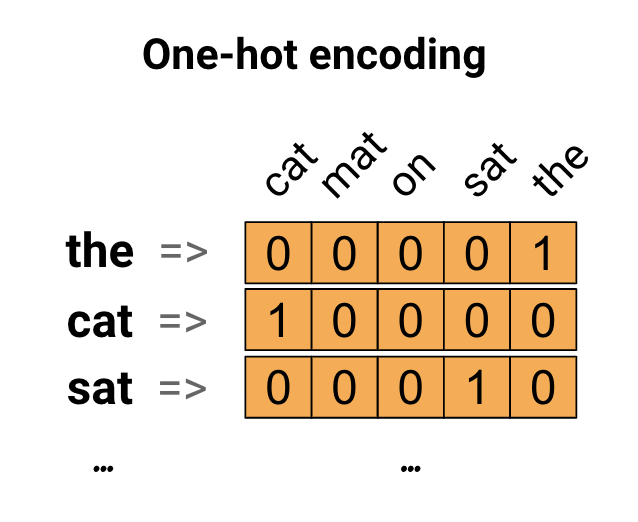
\includegraphics[width=0.5\textwidth]{Figures/one-hot.png}
	\caption{One-hot encoding~\cite{link5}}\label{fig:One-hot encoding}
\end{figure}

\subsection{Využití v praxi One-hot kódování}
V následující ukázce~\ref{src:PythonHot} je prezentována implementace metody pro konverzi lidsky psaného textu do číselných vektorů pomocí one-hot kódování.

\begin{lstlisting}[language=Python,label=src:PythonHot,caption={One-hot kódování v praxi}]
# Převod textu pomocí One-hot kódování
lidsky_text = [
	"Ja jsem nejlepsi ze vsech",
    "Ja jsem nejhorsi ze vsech"
	]

unikatni_slova = set()
for veta in lidsky_text:
    for slovo in veta.split():
        unikatni_slova.add(slovo)
    ...

slovnik = {}
for unikatni_index, unikatni_slovo in enumerate(unikatni_slova):
    one_hot_encoding_vektor = [0] * len(unikatni_slova)
    one_hot_encoding_vektor[unikatni_index] = 1
    slovnik[unikatni_slovo] = one_hot_encoding_vektor
    ...
\end{lstlisting}

V uvedené ukázce je představeno vytvoření slovníku, kde každé unikátní slovo je převedeno na číselný vektor pomocí metody one-hot kódování.
Níže~\ref{src:One-hot encoding} je příklad reprezentace několika slov ve slovníku:

\begin{lstlisting}[label=src:One-hot encoding,caption={One-hot kódování prezentace výsledného formátu dat}]
nejhorsi  : [1, 0, 0, 0, 0, 0]
ze        : [0, 1, 0, 0, 0, 0]
Ja        : [0, 0, 1, 0, 0, 0]
nejlepsi  : [0, 0, 0, 1, 0, 0]
jsem      : [0, 0, 0, 0, 1, 0]
vsech     : [0, 0, 0, 0, 0, 1]
\end{lstlisting}

\section{Vkládání slov}
Vkládání slov (word embedding) je pokročilá metoda pro převod lidsky psaného textu do číselného vektoru, která nahrazuje one-hot kódování. Tato metoda, která se využívá i v praktické části této práce, umožňuje reprezentovat slova pomocí vektorů s desetinnými čísly. Každé číslo ve vektoru reprezentuje různé vlastnosti a vztahy mezi slovy.

Pro výpočet těchto vektorů se používají různé metody, které umožňují zachytit kontext slov a jejich vztahy.
Na rozdíl od one-hot kódování, kde každé slovo má pouze jedinou hodnotu 1 ve vektoru, vkládání slov přináší bohatší informace o kontextu daného slova v textech.

Vkládání slov~\cite{link5}~\ref{fig:Word embedding} má také vlastnost vysoce dimenzionální reprezentace slov, pomocí které zachycuje kontext, ve kterém se slova vyskytují.
Tato vylepšená metoda umožňuje strojům, zpracovávající přirozený jazyk, pracovat s dodatečnými informacemi o podobnosti slov.

Díky technice vkládání slov mají stroje větší schopnost porovnávat a porozumět podobnosti mezi slovy na základě jejich kontextu. To přináší vylepšení v oblasti zpracování přirozeného jazyka a umožňuje lépe porozumět lidsky psanému textu.

\begin{figure}[H]
	\centering
	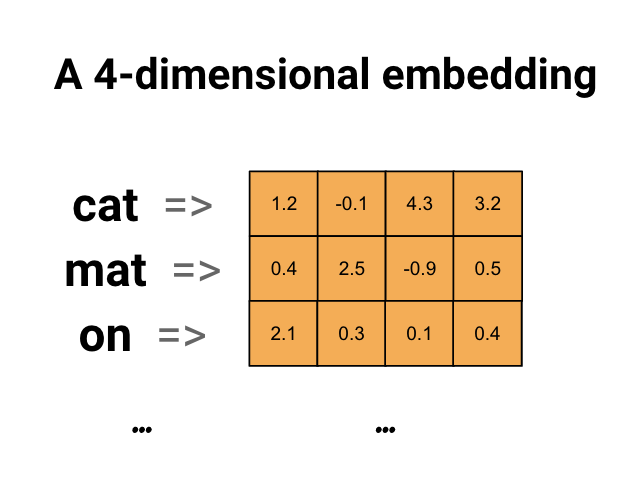
\includegraphics[width=0.6\textwidth]{Figures/embedding2.png}
	\caption{Word embedding~\cite{link5}}\label{fig:Word embedding}
\end{figure}

\subsection{Word2Vec}
Word2Vec~\cite{link6} je významným příkladem modelu pro vytváření vkládání slov~\cite{link5} a byl vyvinutý Tomášem Mikolovem z Google. Tento model umožňuje efektivní převod textu do strojové podoby a zachycuje vztahy mezi slovy.

Word2Vec~\ref{fig:Word2Vec predstaveni moznosti} se skládá z několika algoritmů, které jsou schopné naučit se reprezentaci slov. Existují dva hlavní modely pro učení techniky vkládání slov pomocí Word2Vec: Continuous Bag-of-Words (CBOW) a Continuous Skip-gram.

Continuous Bag-of-Words (CBOW) model se snaží předpovědět aktuální slovo na základě okolních slov v kontextu. Naopak, Continuous Skip-gram model se snaží na základě aktuálního slova předpovědět okolní slova v kontextu. Oba tyto modely přispěly k rozvoji výzkumu vkládání slov a převodu textu do strojové podoby.

Nicméně, i přes úspěch Word2Vec se ukázalo, že existuje efektivnější metoda, která dosahuje stejných výsledků. Tato metoda se nazývá GloVe (Global Vectors for Word Representation)~\cite{link18}. GloVe je algoritmus, který kombinuje globální statistiky slov a lokální kontextové informace při vytváření vkládání slov. Tento přístup umožňuje efektivnější a výkonnější reprezentaci slov.

GloVe se stal populární volbou pro vytváření vkládání slov díky své schopnosti zachytit vztahy mezi slovy ve velkých korpusových datech. Tato metoda přinesla další pokrok v oblasti zpracování přirozeného jazyka a významně přispěla k porozumění slov a jejich kontextu strojovými modely.

\begin{figure}[H]
	\centering
	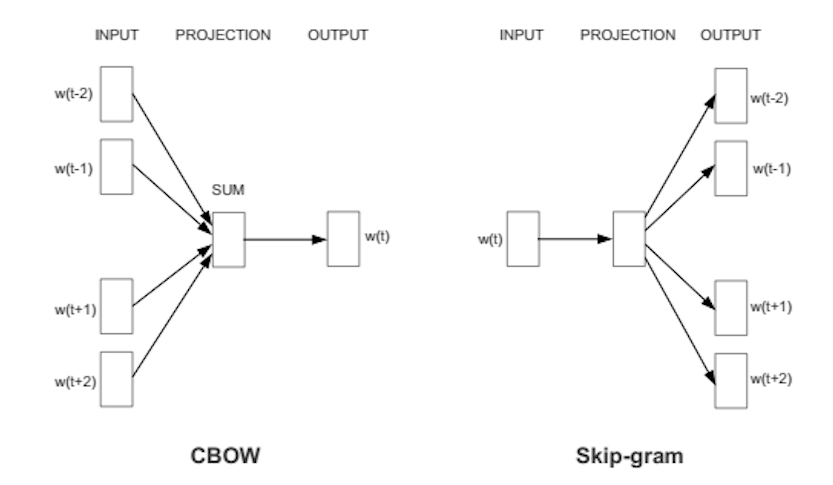
\includegraphics[width=1\textwidth]{Figures/word2vec_diagrams.png}
	\caption{Word2Vec představení možností~\cite{link6}}\label{fig:Word2Vec predstaveni moznosti}
\end{figure}

\section{GloVe}
GloVe (Global Vectors for Word Representation)~\cite{link18} je vylepšeným modelem v porovnání s Word2Vec~\cite{link6} a také vytváří reprezentaci vkládaných slov.
GloVe představuje vylepšenou verzi Word2Vec a přináší několik změn.

Hlavním rozdílem mezi GloVe a Word2Vec je, že GloVe kombinuje obě techniky, Continuous Bag-of-Words (CBOW) a Skip-gram, místo omezení na jednu z nich.
Tímto způsobem GloVe získává výhody obou přístupů.

GloVe je založen na počtu výskytů (count-based).
Tento model se učí vytvářet vkládání slov pomocí redukce dimenzí na matici počtů společných výskytů slov.
Nejprve se vytvoří velká matice, ve které jsou zachyceny informace o tom, jak často se slova vyskytují v různých kontextech ve vstupních datech.
Poté je tato matice převedena na matici nižší dimenze, kde každý řádek představuje vektorovou reprezentaci jednoho slova.

V případě GloVe je matice počtů normalizována vzhledem k počtu výskytů a následně upravena pomocí log-smoothing techniky. GloVe produkuje reprezentaci vkládaných slov, která je kontextově nezávislá, což znamená, že každé slovo je reprezentováno pouze jedním 1D vektorem, který sdružuje různé vlastnosti a vztahy tohoto slova ve vstupním textu. GloVe je také model založený na slovech (word-based), což znamená, že přijímá slova jako vstupní data a generuje vkládání slov jako výstup.

GloVe a Word2Vec se obecně podobně chovají a dosahují podobných výsledků. Výhodou GloVe je však snadnější implementace paralelizace, což vede k vyšší efektivitě.

Vytvořená reprezentace vztahů mezi jednotlivými slovy lze pochopitelněji vypozorovat z obrázku~\ref{fig:GloVe reprezentace slov ve 2D prostoru} 
\begin{figure}[H]
	\centering
	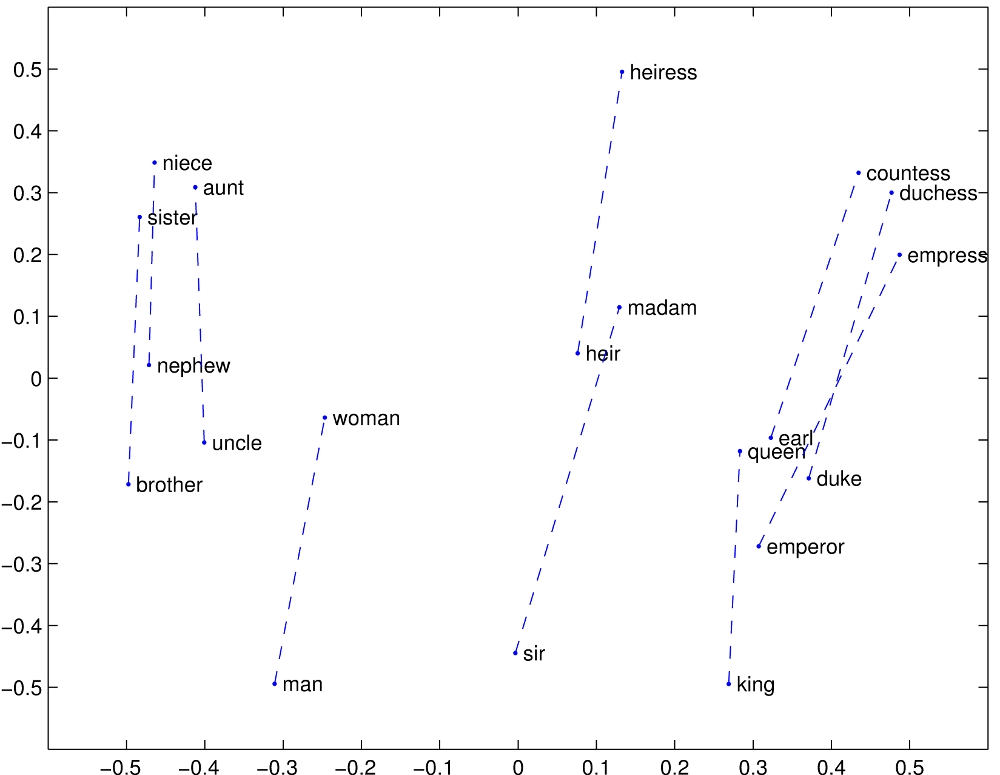
\includegraphics[width=0.8\textwidth]{Figures/GloVe_representation.jpg}
	\caption{GloVe reprezentace slov ve 2D prostoru~\cite{link18}}\label{fig:GloVe reprezentace slov ve 2D prostoru}
\end{figure}

\subsection{Continuous Bag-Of-Words}
Continuous Bag-Of-Words (CBOW)~\cite{link12} je model strojového učení používaný pro vytváření reprezentace vkládaných slov.
Jeho hlavním cílem je předpovědět cílové slovo na základě kontextu, který je definován jako určitý počet slov před a za daným slovem v textu.
CBOW se snaží naučit vektory slov, které mají kvalitní reprezentace pro předpovídání cílových slov na základě kontextuálního významu.

\subsection{Skip-gram}
Metoda Skip-gram~\cite{link13} je další volbou pro model Word2Vec a také je používána společně s CBOW v GloVe.
Hlavním rozdílem mezi Skip-gram a CBOW je v tom, co tyto metody přesně předpovídají.

CBOW předpovídá slovo na základě jeho okolí.
Zkouší určit, jaké slovo by se nejlépe hodilo do středu daného okolí na základě kontextu.
Například, pokud bylo okolí slova `auto' ve větě `Rychle jedoucí auto předjelo nákladní vozidlo' CBOW se snaží předpovědět slovo `rychle' na základě slov `jedoucí' a `předjelo'.

Na druhou stranu, metoda Skip-gram předpovídá okolí daného slova.
Zkouší určit, jaká slova by se mohla objevit v okolí daného slova na základě kontextu.
Pokračujeme-li v příkladu věty `Rychle jedoucí auto předjelo nákladní vozidlo', Skip-gram by se snažil předpovědět slova `jedoucí' a `předjelo' na základě slova `auto'.

\subsection{CBOW a Skip-gram porovnání}
V rámci modelu Word2Vec je metoda CBOW rychlejší, protože zpracovává celý kontext jako jednu entitu.

Metoda Skip-gram vytváří různé páry slov pro každé slovo v kontextu.
Každý pár se skládá z jednoho vstupního centrálního slova a jednoho výstupního okolního slova.
Skip-gram se snaží předpovědět okolní slova na základě daného centrálního slova.

Nicméně, výběr mezi metodou CBOW a Skip-gram závisí na konkrétních úkolech a datových sadách.
Obě metody mají své výhody a omezení a jejich volba závisí na konkrétních potřebách a podmínkách aplikace.

\endinput
\chapter{Neuronové sítě}
Neuronové sítě (Neural Network)~\cite{link1}~\cite{link20} jsou výpočetní modely inspirované biologickým mozkem.
Základními stavebními jednotkami neuronové sítě jsou neurony, které mají své vstupy, váhy a výstup.

Každý neuron obdrží vstupní data od jiných neuronů, přičemž každému vstupu je předána určitá váha.
Váhy slouží k určení důležitosti jednotlivých vstupů.
Neuron zpracovává své vstupní data pomocí aktivačních funkcí a provede sumaci vážených vstupů.
Výsledek této operace je pak předán dalším neuronům jako výstup.

Je důležité poznamenat, že neuronový model~\ref{fig:Model neuronu} může mít libovolný počet vstupů a váh, ale každý neuron generuje pouze jeden výstup.
Tímto způsobem se vytváří komplexní sítě neuronů, které spolupracují při zpracování informací a řešení problémů.

Neuronové sítě se využívají v mnoha oblastech umělé inteligence a strojového učení.
Jejich schopnost zpracovávat složité vzorce a adaptovat se na data je důležitá pro úspěšné řešení rozmanitých úloh, jako je rozpoznávání obrazu, překlad textu, predikce a další.

\begin{figure}[H]
	\centering
	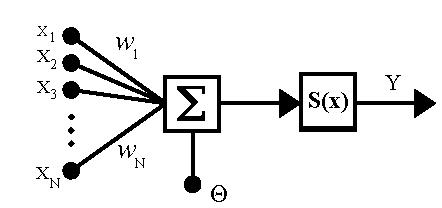
\includegraphics[width=0.6\textwidth]{Figures/NeuronModel.jpg}
	\caption{Model neuronu~\cite{link1}}\label{fig:Model neuronu}
\end{figure}

V následujícím vzorci je formule podle McCulloch–Pitts modelu neuronu.
Váhy se zde násobí společně se vstupními daty, které se následně sčítají a upravují podle parametrizované hodnoty tzv.\ biasu.
Výsledek se vkládá do aktivační funkce a vychází výstup, který se posílá na vstup následujícímu neuronu.

\[Y = S(\sum_{i=1}^{N}(W_{i} X_{i}) + \Theta)\]

\begin{itemize}
\item $X$: vstupní data
\item $W$: váhy mezi neurony
\item $\Theta$: threshold obvykle pod jménem bias
\item $S(x)$: aktivační funkce
\item $Y$: výstup neuronu
\end{itemize}
Proces, při kterém se vstupní data postupně předávají z jednoho neuronu na druhý až k výstupu, se nazývá dopředná propagace (forward propagation).

Při dopředné propagaci se vstupní data předají do prvního neuronu, který provede výpočet pomocí aktivační funkce a váh a výsledek předá jako výstup druhému neuronu.
Tento proces se opakuje, dokud výstup nedorazí ke konečnému neuronu nebo výstupní vrstvě neuronové sítě.

\section{Učení neuronové sítě}
Cílem neuronové sítě je optimalizovat své váhy a biasy tak, aby dosahovala co nejlepších výsledků na základě trénovacích dat.
Trénovací data jsou data, která slouží k učení a nastavení parametrů sítě tak, aby byla schopna správně predikovat výstupy pro nová, dosud neviděná data.

Proces trénování neuronové sítě obecně probíhá ve třech fázích:

Dopředná propagace (Forward propagation): Vstupní data jsou předána sítí, která je pomocí váh a biasů upravuje a předává z neuronu na neuron až k výstupní vrstvě.
V této fázi se vypočítávají aktivační funkce a výstupy jednotlivých neuronů.

Zpětná propagace (Backward propagation): Po provedení dopředné propagace se porovnávají výstupy sítě s očekávanými výstupy na základě trénovacích dat.
Mezi těmito výstupy je propagována zpět skrze síť a jsou vypočítány gradienty, které udávají směr a míru, pomocí jaké je potřeba upravit váhy a biasy jednotlivých neuronů.
    
Aktualizace váh: Na základě gradientů zpětné propagace jsou aktualizovány váhy a biasy neuronů, aby byly přizpůsobeny tak, aby minimalizovaly chybu mezi výstupy sítě a očekávanými výstupy.
Tím se zlepšuje schopnost sítě predikovat správné výstupy.

Tento proces trénování se opakuje pro každou trénovací sadu dat, aby se síť co nejlépe přizpůsobila dané úloze.
Cílem je dosáhnout co nejnižší chyby na trénovacích datech a zároveň dosáhnout schopnosti generalizovat a správně predikovat výstupy i pro nová, dosud neviděná data (testovací či provozní data).

\subsection{Učení pod dohledem}
Při trénování pod dohledem (supervised) neuronové sítě jsou použita trénovací data jako vzor, na základě kterého je pomocí aktuálních nastavení vah a biasů vypočten výstup sítě viz.~dopředná propagace.
Tento výstup je následně porovnán s požadovaným výstupem a vypočtena chyba, která udává rozdíl mezi predikovaným a očekávaným výstupem viz.~zpětná propagace.

\subsection{Volné učení}
Volné učení (unsupervised) je typ učení, kde trénovací data nejsou doprovázena předem danými a chtěnými výstupy.
Na rozdíl od učení pod dohledem (supervised), kde jsou k dispozici páry vstupů s požadovanými výstupy, učení bez dohledu se snaží najít vzorce, struktury nebo skryté informace ve vstupních datech samotných.

Při učení bez dohledu je modelu předloženo pouze množství neoznačených trénovacích dat.
Cílem je objevit struktury, shluky, vzory nebo jiné charakteristiky v datech, aniž by byly předem specifikovány.
Model se učí tím, že přizpůsobuje své váhy a biasy tak, aby optimalizoval určité cílové kriterium, jako je minimalizace chyby nebo maximalizace pravděpodobnosti dat.

\section{Rekurentní neuronové sítě}
Rekurentní neuronové sítě (Recurrent neural network -~RNN)~\cite{link16} jsou architekturou neuronových sítí, která je navržena speciálně pro práci se sekvenčními daty.
Sekvenčními daty se rozumí data, která mají určitý časový nebo prostorový kontext a jsou uspořádána ve formě sekvence nebo posloupnosti.

Hlavním rysem RNN je schopnost uchovávat vnitřní stav (hidden state) a předávat ho ze vstupní vrstvy do následujících časových kroků.
To znamená, že RNN může zpracovávat a modelovat závislosti a vztahy mezi jednotlivými prvky v sekvenci.

V kontextu sekvencí je RNN schopna zohlednit předchozí vstupy a stav sítě a použít je k výpočtu aktuálního výstupu.
Tím je RNN efektivní pro úkoly, jako je předpovídání dalšího prvku v sekvenci (např.\ predikce dalšího slova ve větě), překlad sekvenčních dat (jako je strojový překlad) nebo analýza sentimentu v textu.

\subsection{Zjednodušeně popsané fungování rekurentní neuronové sítě}
Rekurentní neuronová síť (RNN) pracuje se sekvencemi dat.
V případě věty `Já jsem člověk' by se postupně vkládala jednotlivá slova do sítě a RNN by vytvářela výstupy na základě předchozích informací.

Na začátku sekvence je slovo `Já', které se vloží do sítě, a RNN generuje odpovídající výstup.
Poté se slovo `jsem' spolu s informací z předchozího kroku (výstupem zpracování slova `Já') vkládá do sítě a RNN generuje nový výstup.
Tímto způsobem se postupně zpracovávají všechna slova v sekvenci.

Důležité je, že RNN udržuje vnitřní stav, který slouží k předávání informace mezi jednotlivými časovými kroky.
Při zpracování slova `jsem' se do vstupu RNN přidá i informace z předchozího kroku, která obsahuje informaci o slově `Já'.
Tímto způsobem se RNN postupně `paměťově' obohacuje o předchozí informace.

Na konci sekvence má RNN teoreticky informace o všech předchozích slovech, protože se vnitřní stav přenáší z jednoho kroku na druhý.
Tato schopnost zachytit kontext a závislosti mezi slovy v sekvenci je předností RNN a umožňuje tím efektivně pracovat se sekvenčními daty.

\subsection{Architektura rekurentních neuronových sítí}
Architektura rekurentní neuronové sítě~\ref{fig:RNN architektura} jednoho neuronu vypadá následovně.

\begin{figure}[H]
	\centering
	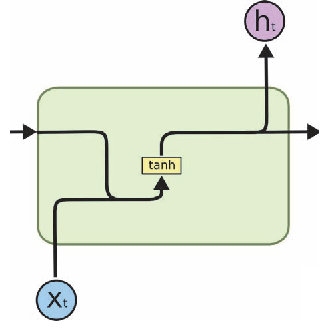
\includegraphics[width=0.3\textwidth]{Figures/RNN_basic_architecture.png}
	\caption{RNN architektura~\cite{link2}}\label{fig:RNN architektura}
\end{figure}

Neuron v rekurentní neuronové síti (RNN) sdílí některé vlastnosti s neurony v běžné neuronové síti.
Do neuronu RNN přicházejí vstupní data ze současného kroku (aktuální vstup) a také data z předchozích kroků (vnitřní stav).

Před zpracováním těchto dat se nad nimi provádí aktivační funkce.
Jednou z běžně používaných aktivačních funkcí v RNN je hyperbolický tangens.
Aktivační funkce hyperbolický tangens převádí vstupní hodnoty na rozmezí mezi -1 a 1.

Aktivační funkce hyperbolický tangens, v následujícím vzorci, se často používá v RNN, protože umožňuje zachování informací z předchozích kroků a přenášení těchto informací do dalších výpočtů.
Díky tomu může RNN efektivně zachycovat závislosti na časové ose a pracovat se sekvencemi dat.

\[h_{t} = \tanh(W_{hh} h_{t-1} + W_{xh} x_{t})\]

\subsubsection{Neduhy rekurentních neuronových sítí}
Rekurentní neuronové sítě (RNN) mají problém s dlouhodobými závislostmi a mizejícím gradientem, což omezuje jejich schopnost efektivně zachycovat dlouhodobé informace v sekvencích dat.

Mizející gradient se projevuje tím, že při zpětném šíření chyby se gradient postupně zmenšuje a při trénování se váhy příliš neaktualizují.
To znamená, že dlouhodobé závislosti mezi vstupy v sekvenci se obtížněji přenášejí a RNN nemusí být schopná se naučit efektivně využívat informace z dávnějších kroků.

Long Short-Term Memory (LSTM) a Gated Recurrent Unit (GRU) jsou vylepšené architektury RNN, které byly navrženy právě s cílem řešit tyto problémy.
Tyto modely používají brány, pro kontrolu probíhajících informací v síti.

LSTM obsahuje speciální paměťovou jednotku, která umožňuje uchovávat a aktualizovat informace na základě brán.
Brány umožňují kontrolovat, které informace jsou považovány za důležité a udržovat je v paměti po delší dobu.

Vylepšení GRU je podobné LSTM, ale s jednodušší architekturou.
Obsahuje aktualizační bránu, která rozhoduje, jak moc má být aktualizovaná paměťová jednotka, a resetovací bránu, která rozhoduje, jakou část paměti zapomenout.
Tímto způsobem se GRU snaží efektivně uchovávat a aktualizovat informace o kontextu.

Tyto vylepšené architektury RNN, jako LSTM a GRU, přinášejí zlepšení v schopnosti zachytit dlouhodobé závislosti a lépe uchovávat kontext při práci se sekvencemi dat.

\section{Long Short-Term Memory}
Long Short-Term Memory (LSTM)~\cite{link3} je speciální verzí rekurentní neuronové sítě, která byla představena v roce 1997 Hochreiterem a Schmidhuberem.

LSTM bylo navrženo specificky k řešení problému s dlouhodobou závislostí a pamatováním informací na delší časový úsek.
Jedním z hlavních problémů standardních rekurentních neuronových sítí je, že mají tendenci rychle zapomenout informace z minulých kroků, což omezuje jejich schopnost zachytit dlouhodobé závislosti v datech.

LSTM využívá speciální strukturu paměťové jednotky, která je schopná efektivně uchovávat a aktualizovat informace na základě brán.
Tato struktura umožňuje paměťové jednotce rozhodovat, které informace mají být zapomenuty a které mají být uchovány na delší dobu.

Díky svému návrhu LSTM~\ref{fig:LSTM architektura} umožňuje neuronové síti uchovávat informace o kontextu na delší časový úsek a lépe pracovat s dlouhými sekvencemi dat.
To přispívá k větší efektivitě a schopnosti modelu zachytit vztahy a závislosti v datech na delších časových škálách.

\begin{figure}[H]
	\centering
	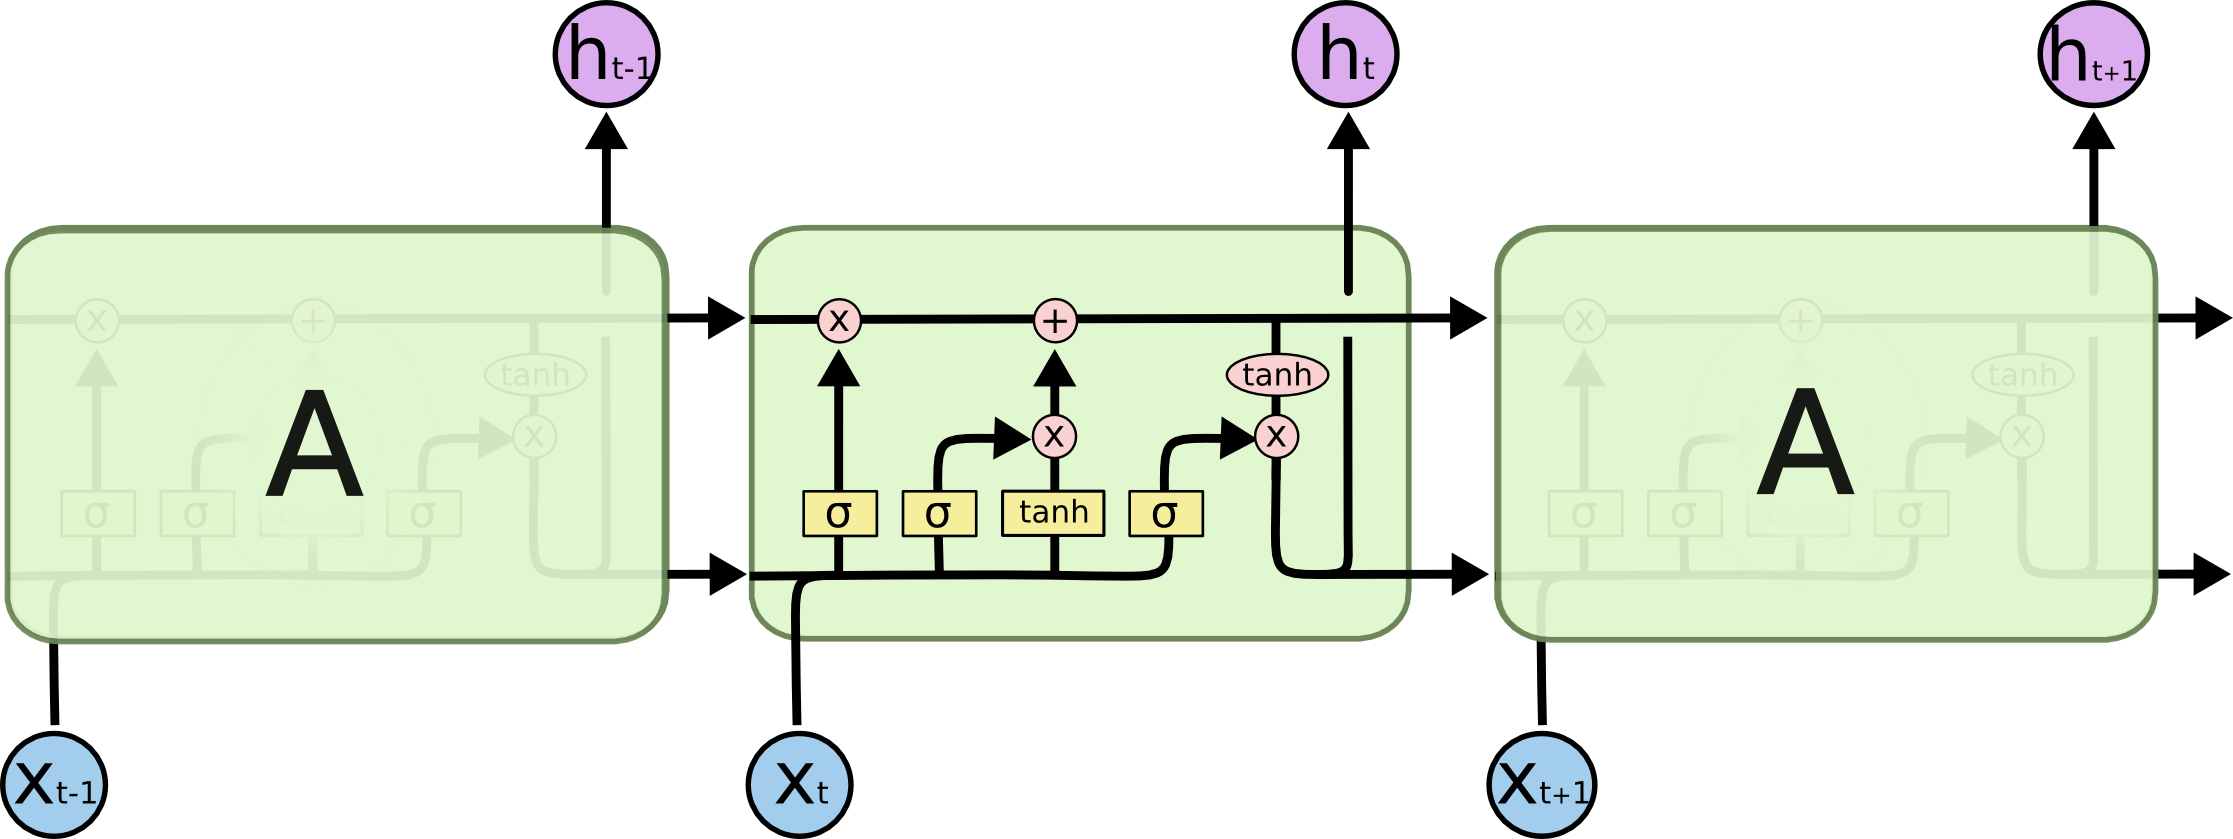
\includegraphics[width=0.8\textwidth]{Figures/LSTM_architecture.png}
	\caption{LSTM architektura~\cite{link3}}\label{fig:LSTM architektura}
\end{figure}

Architektura LSTM je oproti standardní RNN značně komplexnější.
Hlavním rozšířením jsou právě brány~\ref{fig:LSTM architektura neuronu}, které jsou klíčovým prvkem v této architektuře.

\begin{figure}[H]
	\centering
	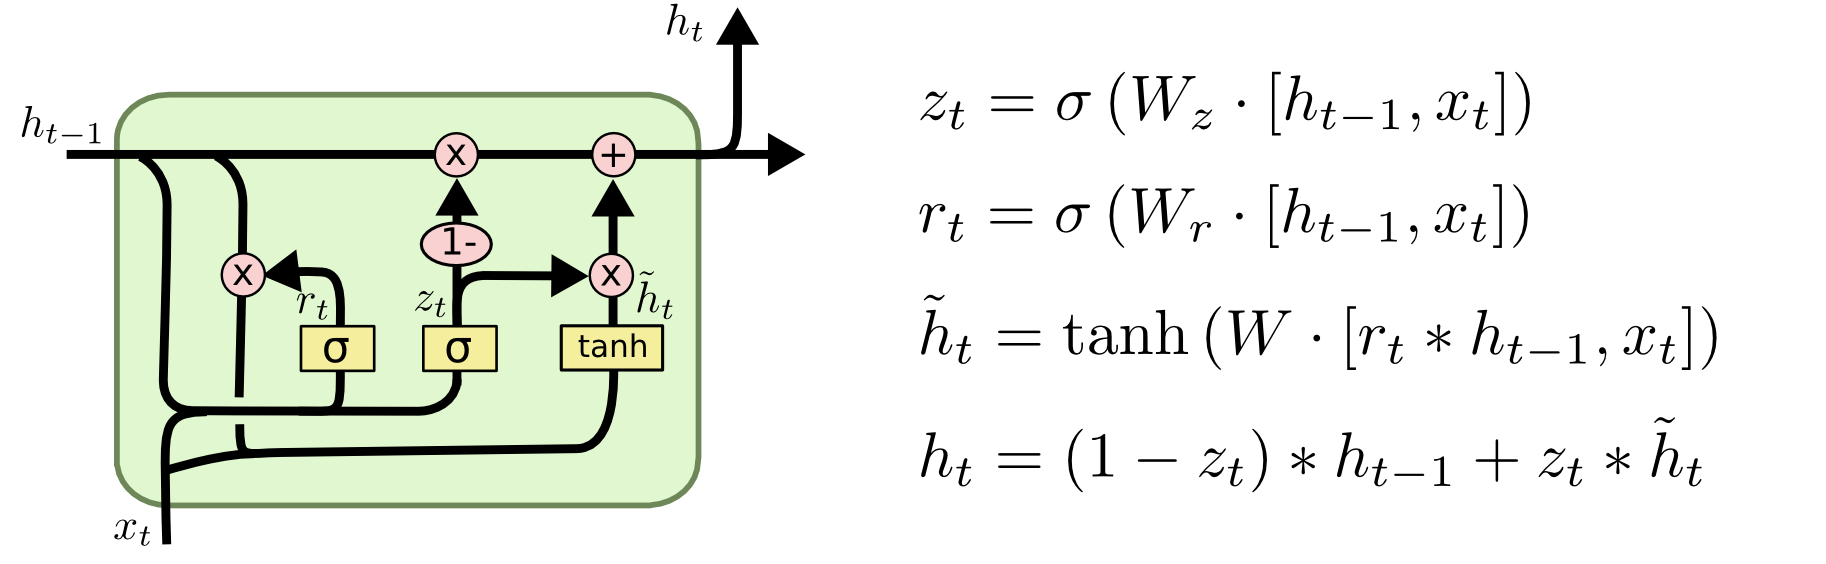
\includegraphics[width=0.8\textwidth]{Figures/LSTM_architecture_neuron.png}
	\caption{LSTM architektura neuronu~\cite{link3}}\label{fig:LSTM architektura neuronu}
\end{figure}

LSTM obsahuje tři základní brány: zapomnětlivou bránu (forget gate), vstupní bránu (input gate) a výstupní bránu (output gate).
Tyto brány spolu s paměťovou jednotkou (memory cell) umožňují LSTM učit se a efektivně pracovat s dlouhodobými závislostmi v datech.
Brány umožňují paměťové jednotce filtrovat a rozhodovat, které informace mají být zapomenuty, které nové informace mají být přidány a které informace mají být využity při výstupu.

\subsection{Zapomnětlivá brána}
Zapomnětlivá brána (forget gate) rozhoduje, jakou část minulého stavu by měl LSTM zapomenout. Na základě vstupů a předchozího stavu určuje, které informace mají být zahozeny.

\subsection{Vstupní brána}
Vstupní brána (input gate) rozhoduje, které nové informace by měly být uloženy v paměťové jednotce LSTM.\@
Pomocí aktivační funkce, využívající sigmoid funkci, určuje, které hodnoty mají být aktualizovány.

\subsection{Výstupní brána}
Výstupní brána (output gate) rozhoduje, jaká část paměťového stavu by měla být odeslána jako výstup z LSTM.\@
Sigmoidová aktivační funkce ovlivňuje, které hodnoty budou výstupem.

\section{Gated Recurrent Unit}
Gated Recurrent Unit (GRU)~\cite{link4} je další speciální verze rekurentní neuronové sítě, která byla představena v roce 2014 Cho et al.
Architektura GRU je navržena k řešení problému mizejícího gradientu, který je běžným problémem standardních RNN.\@

Podobně jako LSTM využívá GRU aktualizační a resetovací brány.
Tyto brány~\ref{fig:GRU architektura neuronu}~\ref{fig:GRU vyznam operaci} umožňují GRU učit se zachovávat informace z dřívějších kroků.
GRU se snaží efektivně zpracovávat dlouhodobé závislosti a současně snižovat problém mizejícího gradientu.

\begin{figure}[H]
	\centering
	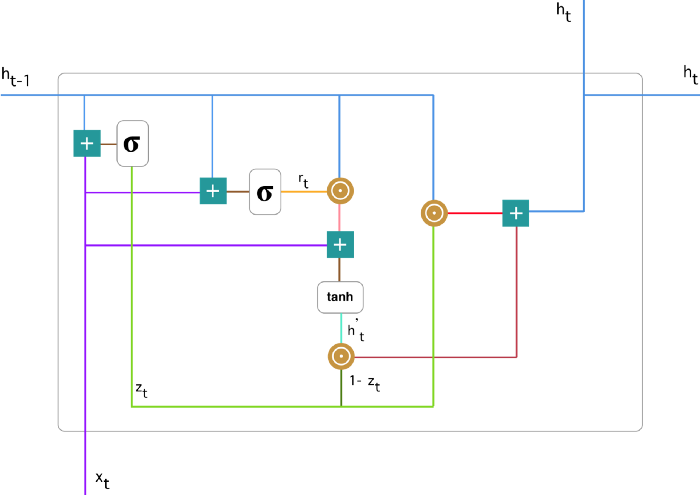
\includegraphics[width=0.8\textwidth]{Figures/GRU_architecture_neuron.png}
	\caption{GRU architektura neuronu~\cite{link4}}\label{fig:GRU architektura neuronu}
\end{figure}

\begin{figure}[H]
	\centering
	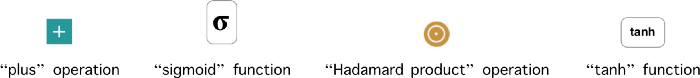
\includegraphics[width=0.8\textwidth]{Figures/GRU_math_operation.png}
	\caption{GRU význam operací~\cite{link4}}\label{fig:GRU vyznam operaci}
\end{figure}

\subsection{Aktualizační brána}
Aktualizační brána (update gate) rozhoduje, jakou část minulého stavu by měla být aktualizována a která část by měla zůstat nezměněna.
Brána pomocí sigmoidové aktivační funkce určuje, jakou část informací z minulého stavu si GRU ponechá a jakou část upraví.

\[z_{t} = \sigma(W^{(z)} x_{t} + U^{(z)} h_{t-1})\]

\subsection{Resetovací brána}
Resetovací brána (reset gate) rozhoduje, jakým způsobem se budou kombinovat vstupní data s předchozím stavem.
Opět pomocí sigmoidové aktivační funkce určuje, které informace se mají resetovat a které se mají zapomenout.

\[r_{t} = \sigma(W^{(r)} x_{t} + U^{(r)} h_{t-1})\]

\subsection{Porovnání}
Vzhledem k popisu problému, jak rozhodnout, zda je text přeložen strojem nebo napsán člověkem, je vhodné využít RNN, konkrétně LSTM a GRU, které jsou navrženy pro zpracování sekvencí dat a řeší problémy původních RNN.\@

LSTM a GRU jsou obě vylepšené architektury RNN, které se snaží překonat problém mizejícího gradientu a zachovat dlouhodobé závislosti v sekvencích.
Oba modely mají některé podobné prvky a často dosahují podobných výsledků.
Obě architektury se liší v počtu a funkcionalitě brán a každá má své výhody.

LSTM je považováno za komplexnější a má větší počet parametrů k učení.
Je navrženo tak, aby si pamatovalo informace z dlouhodobých závislostí a je schopno lépe zachovávat kontext v delších sekvencích.

Na druhou stranu GRU je jednodušší a má menší počet parametrů.
Architektura je navržena tak, aby byla rychlejší a efektivnější v učení.
Je vhodnější pro scénáře, kde je omezený počet trénovacích dat nebo kde je důležitá výpočetní efektivita.
\endinput
\chapter{Popis sítě Transformer}
Transformer byl poprvé představen výzkumným týmem z Google Brain~\cite{link31} v roce 2017 v článku s názvem `Attention Is All You Need' (Pozornost je vše, co potřebujete)~\cite{link27}.
Tento článek představil novou architekturu založenou na mechanismu self-attention, který se ukázal jako velmi efektivní při zpracování sekvencí a dosáhl vynikajících výsledků v oblasti strojového překladu.

Transformer~\cite{link28}~\cite{link25} je architektura hluboké neuronové sítě, která se zaměřuje na problémy sekvence-na-sekvenci, jako je strojový překlad, generování textu nebo analýza sentimentu.
Byl vyvinut jako alternativa k rekurentním neuronovým sítím, jako je LSTM a GRU, a přinesl s sebou zásadní inovaci v oblasti zpracování přirozeného jazyka.

Hlavním stavebním prvkem Transformer sítí je self-attention mechanismus, který umožňuje modelu přidělovat váhu různým slovům v sekvenci na základě jejich vzájemného vztahu a kontextu.
Tímto způsobem si Transformer dokáže lépe poradit s dlouhodobými závislostmi v sekvencích a zachovat informace o kontextu.

Transformer se skládá z několika vrstev sítě obsahujících self-attention mechanismus a další bloky, jako jsou dopředně šířící se sítě (feed-forward) a normalizační vrstvy.
Model je trénován pomocí mechanismu nazvaného `masked multi-head attention' a optimalizován na základě ztrátové funkce, jako je například cross-entropy.

\section{Vlastnosti}
Transformer je navržen pro zpracování sekvenčních dat, včetně vět v přirozeném jazyce.
Jedním z hlavních rozdílů mezi Transformer sítěmi a RNN je právě schopnost Transformer sítí zpracovávat veškerá vstupní data najednou, zatímco RNN musí pracovat sekvenci po sekvenci.
Díky mechanismu self-attention dokáže Transformer přiřadit kontext a důležitost jednotlivým slovům v sekvenci, což umožňuje zpracování celých vět najednou.

Díky této vlastnosti má Transformer výhodu v paralelizaci, protože může zpracovávat vstupní data paralelně na větší části modelu.
To vede k výraznému zrychlení trénování modelu bez ztráty výkonu.
Oproti tomu u RNN je paralelizace složitější kvůli nutnosti zpracovávat data postupně.

Transformer také využívá techniky pozičního kódování (position encoding) pro zachycení kontextu a pozice jednotlivých slov ve vstupní sekvenci.
Pomocí mechanismu attention dokáže mapovat vztahy mezi slovy a lépe porozumět významu a vztahům ve větě.

Před-trénované modely, jako například BERT nebo GPT, jsou vytrénované na velkých datových souborech a poté mohou být doučeny (fine-tuned) na specifické úlohy.
Tyto modely představují významný pokrok v oblasti zpracování přirozeného jazyka, protože mají již naučené znalosti o kontextu a vztazích mezi slovy, což usnadňuje jejich aplikaci na různé úlohy a vede ke zlepšení výkonu.

\section{Architektura}
Architektura Transformer sítí~\ref{fig:Transformer} je založena na mechanismu self-attention, který umožňuje efektivně přiřadit kontext jednotlivým slovům (tokenům) v sekvenci.
Transformer se skládá z několika klíčových komponent, které jsou kodér (Encoder), dekodér (Decoder), Multi-head Attention a poziční kódování (Positional Encoding).

Transformer je schopen zpracovávat vstupní sekvence najednou, což umožňuje výrazně paralelizovat výpočty a urychlit trénování modelu.
Díky kombinaci self-attention, multi-head attention a dopředného šíření použité v neuronové síti je Transformer schopný efektivně zachytit vztahy mezi slovy a generovat kvalitní výstupy pro různé úlohy, včetně strojového překladu, generování textu a dalších úloh zpracování přirozeného jazyka.

\begin{figure}[H]
	\centering
	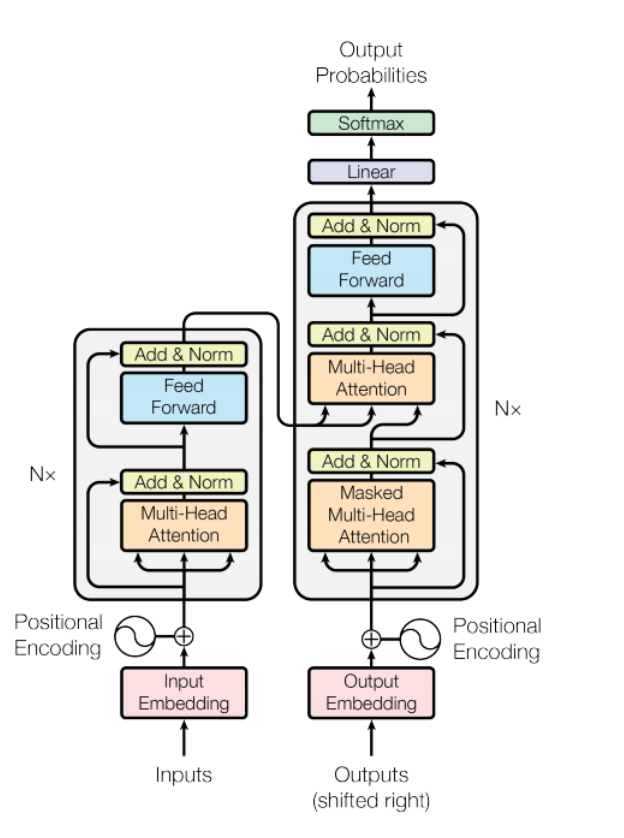
\includegraphics[width=0.6\textwidth]{Figures/transformer_enco_deco.png}
	\caption{Architektura Transformer sítí~\cite{link25}}\label{fig:Transformer}
\end{figure}

\subsection{Kodér}
Kodér (Encoder) převádí vstupní sekvenci (např.\ větu) do vektorové reprezentace.
Skládá se z několika identických vrstev, zvaných kódovacích vrstev (encoder layers).
Každá vrstva obsahuje dvě subkomponenty: multi-head self-attention mechanismus a dopředně šířící se sítě.
Self-attention mechanismus umožňuje modelu získat důležité informace o kontextu jednotlivých slov v rámci sekvence.
Neuronová síť s použitím dopředného šíření slouží k transformaci a kombinaci informací z self-attention mechanismu.

\subsection{Dekodér}
Dekodér (Decoder) generuje výstupní sekvenci (např.\ přeloženou větu) na základě zakódované vstupní sekvence.
Stejně jako kodér, dekodér se skládá z několika identických vrstev, zvaných dekódovací vrstvy (decoder layers).
Každá vrstva obsahuje tři subkomponenty: masked multi-head self-attention mechanismus, který umožňuje dekodéru vidět pouze předchozí pozice, multi-head attention mechanismus, který se zaměřuje na kódovaný kontext, a neuronovou síť pro transformaci a kombinaci informací.

\subsection{Multi-head Attention}
Attention mechanismus je klíčovou součástí sítí Transformer.
Umožňuje modelu přiřadit různou důležitost různým částem vstupní sekvence při generování výstupu.
Transformer používá multi-head attention~\ref{fig:Multi Head Attention}, což znamená, že attention mechanismus je aplikován několikrát s různými projekcemi vstupních vektorů.
To umožňuje modelu získat různé perspektivy na vztahy mezi slovy.

\begin{figure}[H]
	\centering
	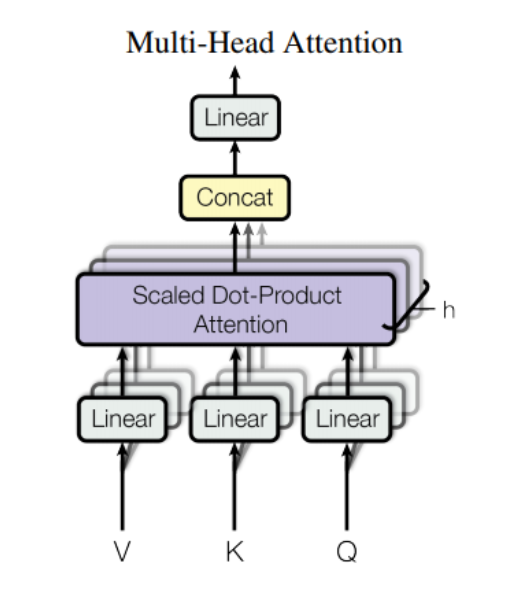
\includegraphics[width=0.6\textwidth]{Figures/multi_head_attention.png}
	\caption{Multi-head Attention~\cite{link25}}\label{fig:Multi Head Attention}
\end{figure}

Každá attention head jednotka využívá tři maticové transformace (Wq, Wk, Wv) pro dotazování (query), klíče (keys) a hodnoty (values) vstupních slov (tokenů).

Výpočet attention se provádí paralelně pro všechny attention head jednotky, což umožňuje efektivní zpracování.
Výsledky z jednotlivých attention head jednotek jsou následně spojeny a předány dále pomocí neuronové sítě využívající dopředné šíření do dalších vrstev transformace.

Tímto způsobem model může získat různé informace o vztazích a relevanci mezi slovy v rámci vstupní sekvence.
Každá attention head jednotka se může zaměřit na specifické aspekty, jako je sledování kontextuálních závislostí, vazeb mezi slovy nebo jiné relevantní informace.

\subsubsection{Počítání techniky Attention}
Transformer využívá scaled dot-product attention~\ref{fig:Scaled Dot-Product Attention} jako mechanismus pro výpočet vah mezi slovy (tokeny) vstupní sekvence.

Při výpočtu scaled dot-product attention jsou vstupní sekvence transformovány pomocí maticových transformací (Wq, Wk, Wv) na dotazovací (query), klíčové (keys) a hodnotové (values) vektory.
Poté se vypočítá podobnost (dot product) mezi dotazovým vektorem a klíčovými vektory.

\begin{figure}[H]
	\centering
	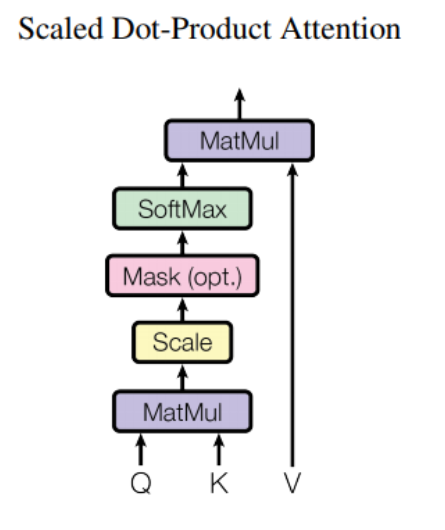
\includegraphics[width=0.6\textwidth]{Figures/scaled_product.png}
	\caption{Scaled Dot-Product Attention~\cite{link25}}\label{fig:Scaled Dot-Product Attention}
\end{figure}

Jedním z klíčových kroků je normalizace podobnosti pomocí škálování, aby se zabránilo problémům s velkými hodnotami např.\ stabilita gradientu.
Následně s využitím Softmax funkce (viz.~následující vzorec) se získávají normalizované váhy pro každý token v rámci sekvence, což reprezentuje jeho relevanci vůči ostatním tokenům.

\[Attention(Q, K, V) = softmax(QK^{T}/\sqrt[2]{d_{k}}) V\]

Následně se váženě kombinují hodnotové vektory (values) s váhami, což vytváří vektor vkládání slov pro každý token v kontextu.
Tento vektor reprezentující vkládána slova~\ref{fig:Vypocet Attention pro sekvenci} obsahuje informaci o samotném tokenu a jeho vztahu k ostatním relevantním tokenům v sekvenci.

\begin{figure}[H]
	\centering
	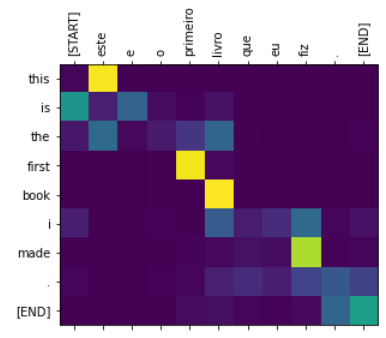
\includegraphics[width=0.6\textwidth]{Figures/attention_example.png}
	\caption{Prezentována technika Attention~\cite{link25}}\label{fig:Vypocet Attention pro sekvenci}
\end{figure}

\subsection{Poziční kódování}
Pro zachycení pořadí slov v sekvenci používá Transformer poziční kódování (positional encoding)~\cite{link38}.
Jedná se o speciální vektorovou reprezentaci, která je přidána ke vstupním slovům (tokenům) a poskytuje informaci o jejich pozici v sekvenci.
Tímto způsobem se zachovává informace o pořadí slov i při zpracování vstupu bez rekurentního propojení.

\subsubsection{Vstupní data}
Ve vstupním procesu Transformer sítí jsou slova reprezentována pomocí techniky vkládání slov, která je často založena na před trénovaných slovních vektorech.
Tyto vektory mají pevnou dimenzi, která se obvykle pohybuje v rozmezí desítek až stovek.

Technika vkládání slov zachycuje významové vztahy mezi slovy, ale nezahrnuje informaci o jejich pozici v sekvenci.
Proto je k zachování informace o pořadí slov v Transformer sítí použita technika nazývaná poziční kódování~\ref{fig:Zobrazeni positional encodingu pro 128D vektor} (viz.~následující~vzorce).

Pozici slov (tokenů) v sekvenci určuje kombinace hodnot vektoru pozičního kódování a vektoru reprezentující vkládána slova.
Tyto informace jsou následně vstupem do kodéru a dekodéru Transformer sítí, který na základě nich provádí operace techniky attention a generuje výstupní sekvenci.

\[PE_{(pos,2i)} = \sin(pos/10000^{2i/d_{model}})\]
\[PE_{(pos,2i+1)} = \cos(pos/10000^{2i/d_{model}})\]

\begin{figure}[H]
	\centering
	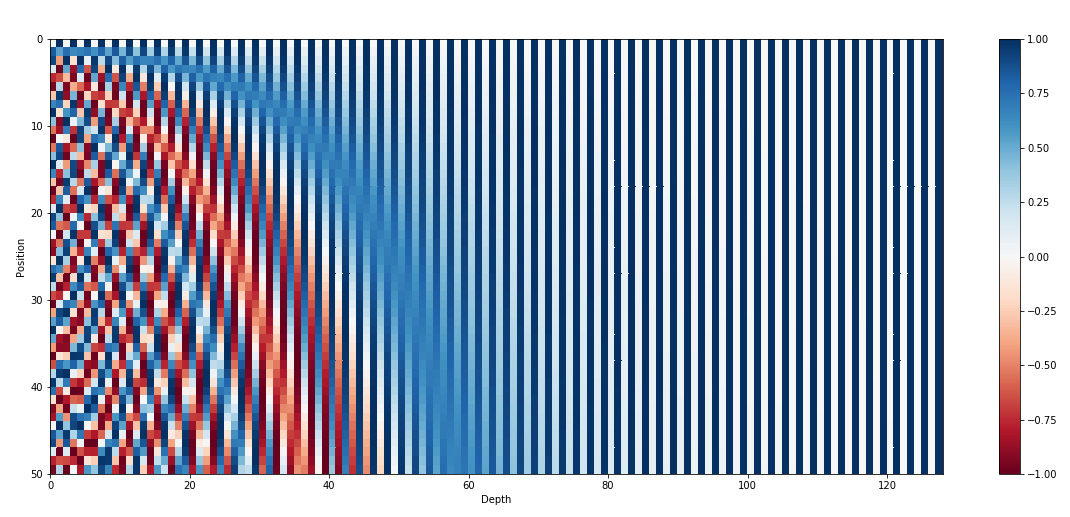
\includegraphics[width=0.6\textwidth]{Figures/positional_encoding.png}
	\caption{Zobrazení Positional Encoding techniky pro 128D vektor~\cite{link38}}\label{fig:Zobrazeni positional encodingu pro 128D vektor}
\end{figure}

\section{Trénování modelu}
Transformer sítě se často učí pod samo dohledem (self-supervised), který kombinuje volné učení (unsupervised) na velkém datovém souboru a následně doučeny (fine-tuned) pomocí učení pod dohledem (supervised).

Při volném učení je Transformer modelu prezentováno velké množství neoznačených dat, například textové korpusy získané z Internetu, které jsou bohaté na přirozený jazyk.
Model se učí predikovat následující slovo v sekvenci, rekonstruovat chybějící části vstupní sekvence nebo provádět jiné úlohy, které vyžadují porozumění kontextu a vztahům mezi slovy.
Tímto učením se model naučí efektivně zpracovávat textová data, zachytávat jazykové vzorce a získávat všeobecné znalosti o vztazích mezi slovy.

Po volném učení trénování je model doučen pomocí dohledového učení na menším označeném datasetu specifickým pro konkrétní úlohu.
Například pro sentimentální analýzu se používá dataset obsahující texty s označeným sentimentem, pro modelování jazyka se používá textový dataset s označenými sekvencemi.

Tímto kombinovaným přístupem se dosahuje dobrého výkonu na konkrétních úlohách zpracování přirozeného jazyka, jako je sentimentální analýza, generování následujících vět, modelování jazyka nebo odpovídání na otázky.
Transformer sítě díky své schopnosti zachycovat kontext a vztahy mezi slovy dosahují v těchto úlohách často nejlepšího (state-of-the-art) výkonu.

\section{Aplikování}
Transformer sítě se ukázaly jako velmi úspěšné v oblasti zpracování přirozeného jazyka a na mnoha úlohách, včetně strojového překladu a časové závislých (time series) předpovědí.
Jejich schopnost zachycovat kontext a vztahy mezi slovy a efektivně zpracovávat sekvence je velmi výhodná pro tyto úlohy.

Nicméně, Transformer sítě mají široké možnosti využití i v jiných oblastech.
Před-trénované modely, jako je GPT-2, se ukázaly jako úspěšné v generování textu, ať už jde o tvorbu nových článků, dialogů, nebo dokonce celých dokumentů.
Díky schopnosti zachycovat kontext a syntaktické struktury vět dokáží tyto modely produkovat texty s vysokou kvalitou a přirozeností.

Transformer sítě se také osvědčily v oblasti analýzy biologických sekvencí, kde jsou schopny zpracovávat sekvence DNA nebo proteinů a hledat vzorce a vztahy mezi nimi.
V oblasti porozumění videím se Transformer sítě využívají k analýze videí a extrakci informací z video sekvencí.

Dalším zajímavým příkladem je využití Transformer sítí v šachových algoritmech, kde mohou být před-trénované modely, jako je GPT-2, doučeny na hrání šachu.
Tyto modely se naučí strategie a pravidla hry a mohou dosahovat vysoké úrovně ve hře proti lidským hráčům.

Transformer sítě tedy nabízejí široké spektrum využití a mohou být adaptovány na různé oblasti, kde je důležité zpracovávat sekvence dat a zachycovat jejich vztahy a strukturu.

\section{BERT}
BERT~(Bidirectional~Encoder~Representations~from~Transformers)~\cite{link29}~\ref{fig:BERT model} je architektura založená na Transformer modelu pro zpracování přirozeného jazyka (NLP).
Byl vytvořen týmem Google~Brain~\cite{link31} a poprvé publikován v roce 2018.

BERT přinesl významný pokrok v oblasti NLP a dosáhl několika nejlepších (state-of-the-art) výsledků v různých NLP úlohách.
Jeho klíčovou vlastností je schopnost zachytit vztahy mezi slovy a jejich kontextem v obou směrech, tedy v předcházejícím i následujícím kontextu.
Tímto způsobem BERT vytváří velmi bohaté a reprezentativní vektorové reprezentace slov a vět.

Díky své schopnosti zachytit jazykový kontext se BERT stal populárním a v roce 2020 byl hojně využíván ve strojovém překladu z anglického jazyka do jiných jazyků.
Jeho před-trénované váhy a modelové znalosti umožňují efektivní adaptaci na různé úlohy pomocí doučující techniky.

BERT otevřel cestu pro další vylepšené architektury v oblasti NLP.\@
Tato architektura se stala důležitým nástrojem pro různé úlohy zpracování přirozeného jazyka, včetně strojového překladu, rozpoznávání entit, sentiment analýzy a dalších.

Původně veřejně publikován BERT má dva typy konfigurace pro sdílení.

\begin{itemize}
\item BERT BASE, který obsahuje 12 enkodéru s 12ti self-attention head jednotkami
\item BERT LARGE s 24 enkodéry a 16ti self-attention head jednotkami
\end{itemize}

BERT je přetrénován na neoznačených (unsupervised) jazykových reprezentacích, což znamená, že trénovací data, na kterých je trénován, nejsou specificky označena pro určitý výstup.
Místo toho jsou použity rozsáhlé textové korpusy, které byly získány ze stránek jako jsou např. Wikipedie a BooksCorpus, které obsahují obecný textový materiál z různých zdrojů.

Díky před trénování na rozsáhlých a různorodých textových korpusů BERT získává obecné jazykové znalosti, které mu umožňují lépe porozumět a reprezentovat různé textové vstupy.
Tato schopnost představuje výhodu při aplikacích NLP, kde je modelu potřeba porozumět a zachytit různé jazykové nuance a vztahy.

BERT bere v potaz kontext slova, což mu umožňuje rozlišovat význam slova v závislosti na jeho kontextu.
Rozdíl ve významu slova `koruna' v následujících větách by měl být reflektován v reprezentaci chování BERT modelu.

\begin{itemize}
\item Česká koruna se propadla nejvíce v historii ČR.
\item V korunách stromů sedí ptáci.
\item Král nosí korunu.
\end{itemize}

BERT je obousměrným (bidirectional) modelem, což znamená, že bere v potaz kontext slova z obou směrů.
Tato vlastnost je dosažena pomocí mechanismu nazývaného maskované modelování jazyka (masked language modeling), kdy BERT se učí předpovídat chybějící slova v textu.
Při trénování jsou náhodně vybraná slova věty maskována a model se učí předpovídat původní tvar těchto slov na základě kontextu, který zahrnuje jak slova před nimi, tak slova za nimi.

Díky obousměrnému zohledňování kontextu je BERT schopen zachytit slovní vztahy a významy ve větách, které jsou důležité pro porozumění celému textu.
Tím se odstraňuje omezení jednosměrných (unidirectional) modelů, které sledují kontext pouze z jednoho směru.
Obousměrný přístup BERTa umožňuje lépe modelovat závislosti mezi slovy a vytvářet kontextuální reprezentace jednotlivých slov na základě celé věty.

\begin{figure}[H]
	\centering
	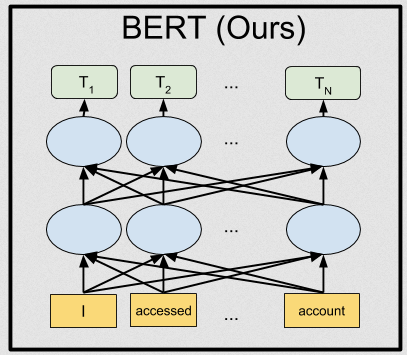
\includegraphics[width=0.6\textwidth]{Figures/BERT.png}
	\caption{BERT model~\cite{link24}}\label{fig:BERT model}
\end{figure}

\subsection{Ukázka obousměrného přístupu}
V následující větě `Já jsem Honza' BERT s obousměrným přístupem je schopen zachytit vztah slova `jsem' nejen k předchozímu slovu `Já', ale také k následujícímu slovu `Honza'.
Díky své schopnosti zohledňovat kontext z obou směrů dokáže BERT lépe porozumět vztahům mezi slovy ve větě.

V případě jednosměrného modelu by pouze kontext předcházející slovu `jsem' nebo kontext následující slova `jsem' byl brán v úvahu při modelování vztahu s tímto slovem.
To by mohlo vést k omezenému porozumění celému kontextu věty.

Díky schopnosti BERTa zohledňovat kontext ze všech stran je schopen zachytit významy obou slov `Já' a `Honza' a lépe reprezentovat jejich vzájemný vztah ve větě `Já jsem Honza'.
Tímto způsobem BERT dokáže lépe porozumět významům jednotlivých slov a jejich vztahům v celém kontextu věty.

Jednosměrný přístup, který je běžně používán v tradičních jazykových modelech, neumožňuje předvídat budoucí slova na základě slov, která jej předcházela a následovala.
Tím pádem by při jednosměrném modelování nebylo možné získat úplný kontext věty.

BERT řeší tento problém pomocí techniky maskování (masking)~\ref{fig:BERT maskovani}.
Při trénování BERTa jsou náhodně vybraná slova vstupního textu maskována a následně je model trénován na předpovídání těchto zakrytých slov na základě okolního kontextu.
Tímto způsobem BERT získává schopnost porozumět kontextu celé věty a naučit se předpovídat nejen slova na základě předchozích, ale i na základě budoucích slov, která jsou v daném kontextu maskována.

\begin{figure}[H]
	\centering
	
\includegraphics[width=1\textwidth]{Figures/BERT_bi.png}
	\caption{BERT případ maskování~\cite{link24}}\label{fig:BERT maskovani}
\end{figure}

Technika maskování slov ve vstupním textu a následná predikce těchto slov je známá už delší dobu.
Co je unikátní u BERTa, je jeho schopnost efektivně využívat tuto techniku v kombinaci s obousměrným kontextovým modelováním.

Co se týče porozumění vztahům mezi větami, BERT má v sobě zakódovanou informaci o vzájemném vztahu dvou vět v tzv.\ segmentovém vektoru (segment embedding vector).
Segmentový vektor~\ref{fig:BERT priklad sekvence} je část reprezentace vstupního textu, která specifikuje, které slova a věty patří do kterých segmentů.
BERT je tak schopen rozpoznat, zda věta `A' následuje po větě `B' nebo naopak.

\begin{figure}[H]
	\centering
	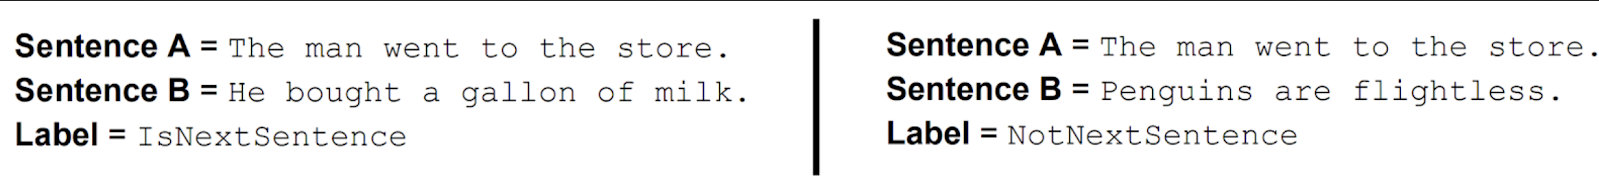
\includegraphics[width=1\textwidth]{Figures/BERT_sequence.png}
	\caption{BERT příklad sekvence~\cite{link24}}\label{fig:BERT priklad sekvence}
\end{figure}

\subsection{Využití}
Jedna z výhod Transformer sítí je možnost využití před-trénovaných modelů pro různé úlohy zpracování přirozeného jazyka.

Před-trénované modely jako je BERT jsou natrénovány na obrovských množstvích textových dat a jsou schopny zachytit bohaté vztahy mezi slovy a kontextem.
Tyto modely jsou takovým druhem jazykového modelu, který vytváří vektorové reprezentace slov a vět na základě jejich kontextu.

Pomocí techniky doučení je možné před-trénovaný model BERT přizpůsobit na specifický úkol, například pro rozpoznávání sentimentu, strojový překlad nebo jiné úlohy zpracování přirozeného jazyka.
Při doučování se upravují pouze některé části modelu, zatímco váhy a znalosti z před trénované fáze zůstávají zachovány.

\endinput
\chapter{Detekce strojově přeložených textů}
Pro praktickou ukázku byl celý kód napsán v programovacím jazyce Python~\cite{link38} s hlavním využitím knihovny Tensorflow.
Jako prostředí pro testování byl zvolen Google Colab~\cite{link33}, ale pro rozsáhlejší testování byl využit školní server VŠB.

Pro tuto praktickou ukázku byly vybrány dva různé datové soubory.
První soubor obsahuje pouze anglický jazyk, zatímco druhý soubor obsahuje texty ze 24 různých jazyků.

Pro každý z těchto datových souborů bylo vytvořeno několik modelů~\ref{Typy modelu}, které byly dále pozorovány a laděny.
V následující části budou uvedeny výsledky těchto modelů pro každý datový soubor.

\begin{itemize}\label{Typy modelu}
    \item LSTM model
    \item GRU model
    \item LSTM model s technikou GloVe embedding
    \item GRU model s technikou GloVe embedding 
    \item LSTM model s technikou Attention
    \item GRU model s technikou Attention
    \item BERT
\end{itemize} 

\section{Postup pro vytvoření klasifikátorů}
\begin{itemize}\label{Postup}
    \item Příprava trénovacího datasetu: Nejprve je zapotřebí mít k dispozici trénovací dataset, který obsahuje textová data a odpovídající klasifikační štítky. Dataset by měl být rozdělen na trénovací, validační a testovací část.
    \item Předzpracování dat: Textová data musí být převedena do vhodného formátu pro zpracování strojem. To zahrnuje tokenizaci textu.
    \item Vytvoření vektorové reprezentace: Textová data musí být reprezentována pomocí vektorů, které jsou zpracovatelné strojem. K tomu se často využívá technika vkládání slov (word embeddings), která převádí tokeny na vektorovou reprezentaci. Využije se čistě vytvořená reprezentace vkládání slov z trénovacího datasetu a GloVe.
    \item Návrh architektury klasifikátoru: Je třeba vybrat vhodnou architekturu klasifikátoru, která bude použita pro trénování. Mezi běžné architektury pro klasifikaci textu patří rekurentní neuronové sítě (např. LSTM, GRU) nebo transformer modely (jako BERT).
    \item Trénování klasifikátoru: Architektura klasifikátoru je trénována na trénovacím datasetu pomocí metody zpětného šíření chyby (backpropagation). Během trénování jsou optimalizovány váhy a biasy modelu tak, aby minimalizovaly chybu při predikci klasifikačních štítků. Trénování může probíhat po několik epoch, přičemž v každé epoše jsou data prezentována modelu v různém pořadí (pro lepší generalizaci).
    \item Optimalizace a ladění modelu: Po dokončení trénování je třeba model optimalizovat a ladit. To může zahrnovat úpravu hyperparametrů modelu (např.~learning~rate, velikost skrytých vrstev, počet vrstev), aplikaci regularizace (např.~dropout,~Gaussovský~dropout) a další techniky pro zvýšení výkonnosti a generalizace modelu.
    \item Evaluace modelu: Model je vyhodnocen na validačním a testovacím datasetu pomocí metriky přesnosti. Na základě výsledků je možné porovnávat různé klasifikátory a vybrat ten nejlepší.
	\item Inferenční fáze: Po úspěšném trénování a vyhodnocení je model připraven k použití pro predikce na nových neznámých datech. Je možné jej aplikovat na reálné problémy a získat predikce nebo klasifikace na základě nových vstupů.
\end{itemize} 

Celý proces vytváření klasifikátorů je iterativní a zahrnuje opakované testování, ladění a optimalizaci modelu s cílem dosáhnout co nejlepších výsledků.

\subsection{Datové soubory}
Datové soubory byly vytvořeny autorem této práce.
Na počátku bylo navrženo získání odstavců napsaných lidmi na radu vedoucího práce.
Tato data byla získána z webových stránek Evropské unie~\cite{link35}, které obsahují texty ve všech jazycích, do kterých autoři a překladatelé přispívají.

Po očištění tohoto textového korpusu byla proveden strojový překlad pomocí několika nástrojů, jako je Deepl~\cite{link37} a Google Translate~\cite{link36}.

Aby byl zachován rozdíl mezi reálnými daty a přeloženými daty, bylo stanoveno důležité pravidlo.
Každý odstavec napsaný lidmi byl přeložen pouze do jednoho jazyka, aby byl datový soubor rovnoměrně rozdělen mezi reálná a přeložená data.

\subsection{Dataset pouze s anglickými texty}
Tento dataset obsahuje pouze texty psané v anglickém jazyce, které budou sloužit k trénování klasifikátorů pro provedení detekce. 

V následující tabulce~\ref{tab:English dataset} jsou uvedeny informace o datovém souboru obsahujícím pouze anglicky psané texty. 

Zmenšená velikost přeložených odstavců je způsobena rozdíly v počtu původních odstavců v různých jazycích.
Každý jazyk se liší a také spisovatelé či překladatelé přispívají ke specifičnosti každého jazyka.
\begin{table}[H]
	\centering
	\caption{Rozložení datového souboru pro Angličtinu}\label{tab:English dataset}
	\begin{tabular}{ c c }
			\toprule
			Typ & Počet\\
			\midrule
			Reálné odstavce & 3398\\
			Přeložené odstavce & 3437\\
			\midrule
		\end{tabular}
\end{table}

\subsection{Dataset přeložen do všech jazyků}
Tento datový soubor obsahuje texty napsané ve všech jazycích~\ref{Jazyky EU}, které se vyskytují na stránkách Evropské unie.

Celkový počet jazyků v tomto datovém souboru je 24.
\begin{itemize}\label{Jazyky EU}
    \item Bulgarian, Croatian, Czech, Danish, Dutch, English,
    \item Estonian, Finland, French, German, Greek, Hungarian,
    \item Irish, Italian, Latvian, Lithuanian, Maltese, Polish,
    \item Portuguese, Romania, Slovakia, Slovene, Spanish, Sweden
\end{itemize} 

V následující tabulce~\ref{tab:Multi dataset} jsou uvedeny informace o datovém souboru obsahujícím pouze anglicky psané texty.

\begin{table}[H]
	\centering
	\caption{Rozložení více jazyčného datového souboru}\label{tab:Multi dataset}
	\begin{tabular}{ c c }
			\toprule
			Typ & Počet\\
			\midrule
			Reálné odstavce & 38528\\
			Přeložené odstavce & 38581\\
			\midrule
		\end{tabular}
\end{table}

\subsection{Trénování}
Klasifikátory byly trénovány na základě svých individuálních parametrů a konfigurací, při použití optimálního počtu epoch pro každý z nich.

Po opakovaném trénování klasifikátorů se projevil jev přetrénování na trénovacích datech.
K tomu účelu byly přidány Dropout vrstvy a regularizátory s cílem potlačit tento jev.
Nicméně i přes tyto přidané techniky se nepodařilo přetrénování úplně eliminovat.
Po důkladném zkoumání chování klasifikátorů, které byly přetrénovány, se ukázalo, že detekce na testovacích datech byla lepší než detekce u klasifikátorů, kterým bylo trénování ukončeno před dosažením přetrénování.

Na základě těchto výsledků bylo provedeno upravení trénování všech modelů.
První fáze trénování spočívala v natrénování modelu na omezeném počtu epoch a následně byl vybrán model s nejlepší binární přesností (binary accuracy).
Ve druhé fázi trénování byla použita metoda hrubé síly k dalšímu zlepšení modelu.
V každé epoše byl model přetrénován a poté byl vybrán ten model, který dosáhl lepší hodnoty validační přesnosti (binary validation accuracy).
Tímto přístupem bylo dosaženo postupného zlepšování modelu a výběru nejlepšího možného výsledku.

Díky tomuto dvoucestnému trénování se model nejdříve naučí základní vzorce a struktury z trénovacích dat, což mu umožní získat základní znalosti a porozumění danému problému.
Následně, v druhé fázi trénování, dochází k dalšímu zlepšení modelu pomocí metody hrubé síly.
Tím se zvyšuje jistota, s jakou klasifikátor provádí predikce.

Dvojí trénování tak umožňuje kombinovat přínosy základního naučeného vzorce s vylepšenými schopnostmi a jistotou predikce.

\subsection{LSTM a GRU modely}
Klasifikátor využívá architekturu LSTM (Long Short-Term Memory) nebo GRU (Gated Recurrent Unit) společně s technikou obousměrných vrstev (Bidirectional) pro efektivní zachycení kontextu jednotlivých tokenů.
Pro potlačení přetrénování na trénovacích datech je v klasifikátoru implementována Gaussian-Dropout vrstva.
Optimalizace vah klasifikátoru je prováděna pomocí optimalizátoru RMSprop, který se zaměřuje na adaptivní aktualizaci vah s ohledem na historii gradientů.
Pro aktivační funkci v klasifikátoru byla zvolena Sigmoid, která transformuje výstupy neuronů na pravděpodobnostní hodnoty mezi 0 a 1.

\subsubsection{Technika GloVe}\label{subsec:Technika GloVe}
K modelu LSTM nebo GRU je připojen Embedding, který je odvozen z již natrénovaného vektorového mapování GloVe.
Tímto způsobem bude mít model naučené vztahy mezi slovy, které byly trénovány na rozsáhlejších datových sadách než je samotný trénovací dataset.

K modelu LSTM nebo GRU je přidávána Attention vrstva, která je moderní technikou pro výpočet vah jednotlivých slov v sekvenci.
Tímto způsobem má model možnost porozumět významu jednotlivých slov a upřednostnit ta, která jsou významná.

\subsubsection{Technika Attention}\label{subsec:Technika Attention}
K modelu LSTM nebo GRU je přidávána Attention vrstva, která je moderní technikou pro výpočet vah jednotlivých slov v sekvenci.
Tímto způsobem má model možnost porozumět významu jednotlivých slov a upřednostnit ta, která jsou významná.

\subsection{BERT}
Klasifikátor využívá před-trénovaný model BERT, ke kterému je připojena Dropout vrstva a vrstva neuronové sítě s jedním neuronem pro binární detekci.

\section{Výsledné klasifikátory anglického datasetu}

\subsection{Architektura klasifikátoru LSTM}\label{arch: LSTM}
Samotný model~\ref{tab:LSTM model} se skládá z Embedding vrstvy, který překládá tokeny do 256 dimenzionálního vektoru, následované dvěma obousměrnými LSTM vrstvami, přičemž každá z těchto vrstev obsahuje 128 neuronů.
Poté následují čtyři neuronové vrstvy s postupně se snižujícím počtem neuronů: 64, 32, 16 a 1.
Mezi každou vrstvou modelu se nachází Dropout vrstvy nebo regularizující vrstvy. Pro optimalizaci vah modelu byl zvolen optimalizátor RMSprop a jako výpočetní metrika byla zvolena binární přesnost. 
Celkový počet parametrů modelu činí 3 179 905.

\begin{table}[H]
	\centering
	\caption{LSTM model}\label{tab:LSTM model}
	\begin{tabular}{ c c c }
			\toprule
			Vrstva modelu & výstupný formát dat & počet parametrů\\
			\midrule
            TextVectorization & (None, 256) & 0\\         
            Embedding & (None, 256, 256) & 2 372 352\\   
            Bidirectional & (None, 256, 256) & 394 240\\    
			Gaussian Noise & (None, 256, 256) & 0\\
            Bidirectional & (None, 256) & 394 240\\
			Gaussian Noise & (None, 256) & 0\\
            Dense & (None, 64) & 16 448\\ 
			Gaussian Noise & (None, 64) & 0\\
			Dense & (None, 32) & 2 080\\ 
			Gaussian Noise & (None, 32) & 0\\
			Dense & (None, 16) & 528\\ 
            Dropout & (None, 16) & 0\\   
            Dense & (None, 1) & 17\\ 
			\midrule
		\end{tabular}
\end{table}

\subsection{Architektura klasifikátoru GRU}\label{arch: GRU}
Samotný model~\ref{tab:GRU model} se skládá z Embedding vrstvy, který překládá tokeny do 256 dimenzionálního vektoru, následované dvěma obousměrnými GRU vrstvami, přičemž každá z těchto vrstev obsahuje 128 neuronů.
Poté následují čtyři neuronové vrstvy s postupně se snižujícím počtem neuronů: 64, 32, 16 a 1.
Mezi každou vrstvou modelu se nachází Dropout vrstvy nebo regularizující vrstvy.
Pro optimalizaci vah modelu byl zvolen optimalizátor RMSprop a jako výpočetní metrika byla zvolena binární přesnost.
Celkový počet parametrů modelu činí 2 984 321.

\begin{table}[H]
	\centering
	\caption{GRU model}\label{tab:GRU model}
	\begin{tabular}{ c c c }
			\toprule
			Vrstva modelu & výstupný formát dat & počet parametrů\\
			\midrule
            TextVectorization & (None, 256) & 0\\         
            Embedding & (None, 256, 256) & 2 372 352\\   
            Bidirectional & (None, 256, 256) & 296 448\\    
            Bidirectional & (None, 256) & 296 448\\
            Dense & (None, 64) & 16 448\\ 
			Gaussian Noise & (None, 64) & 0\\
			Dense & (None, 32) & 2 080\\ 
			Gaussian Noise & (None, 32) & 0\\
			Dense & (None, 16) & 528\\ 
            Dense & (None, 1) & 17\\ 
			\midrule
		\end{tabular}
\end{table}


\subsection{Architektura klasifikátoru LSTM s technikou GloVe}\label{arch: LSTM GloVe}
V LSTM modelu je obecná Embedding vrstva nahrazena GloVe Embedding~\ref{tab:LSTM GloVe model} vrstvou viz.~\ref{subsec:Technika GloVe}.
Celkový počet parametrů modelu činí 2 604 009.

\begin{table}[H]
	\centering
	\caption{LSTM model s technikou GloVe }\label{tab:LSTM GloVe model}
	\begin{tabular}{ c c c }
			\toprule
			Vrstva modelu & výstupný formát dat & počet parametrů\\
			\midrule
            Text Vectorization & (None, 256) & 0\\         
            GloVe & (None, 256, 256) & 1 853 800\\   
            Bidirectional & (None, 256, 256) & 336 896\\    
			Gaussian Noise & (None, 256, 256) & 0\\
            Bidirectional & (None, 256) & 394 240\\
			Gaussian Noise & (None, 256) & 0\\
            Dense & (None, 64) & 16 448\\ 
			Gaussian Noise & (None, 64) & 0\\
			Dense & (None, 32) & 2 080\\ 
			Gaussian Noise & (None, 32) & 0\\
			Dense & (None, 16) & 528\\ 
            Dropout & (None, 16) & 0\\   
            Dense & (None, 1) & 17\\ 
			\midrule
		\end{tabular}
\end{table}

\subsection{Architektura klasifikátoru GRU s technikou GloVe}\label{arch: GRU GloVe}
V GRU modelu je obecná Embedding vrstva nahrazena GloVe Embedding~\ref{tab:GRU GloVe model} vrstvou viz.~\ref{subsec:Technika GloVe}.
Celkový počet parametrů modelu činí 2 422 761.

\begin{table}[H]
	\centering
	\caption{GRU s technikou GloVe model}\label{tab:GRU GloVe model}
	\begin{tabular}{ c c c }
			\toprule
			Vrstva modelu & výstupný formát dat & počet parametrů\\
			\midrule
            Text Vectorization & (None, 256) & 0\\         
            GloVe & (None, 256, 256) & 1 853 800\\   
            Bidirectional & (None, 256, 256) & 253 440\\    
			Gaussian Noise & (None, 256, 256) & 0\\
            Bidirectional & (None, 256) & 296 448\\
			Gaussian Noise & (None, 256) & 0\\
            Dense & (None, 64) & 16 448\\ 
			Gaussian Noise & (None, 64) & 0\\
			Dense & (None, 32) & 2 080\\ 
			Gaussian Noise & (None, 32) & 0\\
			Dense & (None, 16) & 528\\ 
            Dropout & (None, 16) & 0\\   
            Dense & (None, 1) & 17\\ 
			\midrule
		\end{tabular}
\end{table}

\subsection{Architektura klasifikátoru LSTM s technikou Attention}\label{arch: LSTM Attention}
Do LSTM modelu~\ref{tab:LSTM Attention model} byla přidána Attention vrstva~\ref{subsec:Technika Attention} a došlo k další změně optimalizátoru z RMSprop na Adam.
Celkový počet parametrů modelu nyní činí 3 180 417.

\begin{table}[H]
	\centering
	\caption{LSTM s technikou Attention model}\label{tab:LSTM Attention model}
	\begin{tabular}{ c c c }
			\toprule
			Vrstva modelu & výstupný formát dat & počet parametrů\\
			\midrule
            Text Vectorization & (None, 256) & 0\\         
            Embedding & (None, 256, 256) & 2 372 352\\   
            Bidirectional & (None, 256, 256) & 394 240\\    
			Gaussian Noise & (None, 256, 256) & 0\\
            Bidirectional & (None, 256, 256) & 394 240\\
			Gaussian Noise & (None, 256, 256) & 0\\
			Attention & (None, 256) & 512\\
			Gaussian Noise & (None, 256) & 0\\
            Dense & (None, 64) & 16 448\\ 
			Gaussian Noise & (None, 64) & 0\\
			Dense & (None, 32) & 2 080\\ 
			Gaussian Noise & (None, 32) & 0\\
			Dense & (None, 16) & 528\\ 
            Dropout & (None, 16) & 0\\   
            Dense & (None, 1) & 17\\ 
			\midrule
		\end{tabular}
\end{table}

\subsection{Architektura klasifikátoru GRU s technikou Attention}\label{arch: GRU Attention}
Do GRU modelu~\ref{tab:GRU Attention model} byla přidána Attention vrstva~\ref{subsec:Technika Attention} a došlo k další změně optimalizátoru z RMSprop na Adam.
Celkový počet parametrů modelu nyní činí 2 984 833.

\begin{table}[H]
	\centering
	\caption{GRU s technikou Attention model}\label{tab:GRU Attention model}
	\begin{tabular}{ c c c }
			\toprule
			Vrstva modelu & výstupný formát dat & počet parametrů\\
			\midrule
            Text Vectorization & (None, 256) & 0\\         
            Embedding & (None, 256, 256) & 2 372 352\\   
            Bidirectional & (None, 256, 256) & 296 448\\    
			Gaussian Noise & (None, 256, 256) & 0\\
            Bidirectional & (None, 256, 256) & 296 448\\
			Gaussian Noise & (None, 256, 256) & 0\\
			Attention & (None, 256) & 512\\
			Gaussian Noise & (None, 256) & 0\\
            Dense & (None, 64) & 16 448\\ 
			Gaussian Noise & (None, 64) & 0\\
			Dense & (None, 32) & 2 080\\ 
			Gaussian Noise & (None, 32) & 0\\
			Dense & (None, 16) & 528\\ 
            Dropout & (None, 16) & 0\\   
            Dense & (None, 1) & 17\\ 
			\midrule
		\end{tabular}
\end{table}

\subsection{Architektura klasifikátoru BERT}\label{arch: BERT}
Tento model~\ref{tab:BERT model} se skládá z několika vrstev: Input vrstvy, preprocessoru pro přetrénovaný model BERT, samotného modelu BERT a přídavné neuronové sítě.
První vrstvou je Input vrstva, která slouží k přijímání textových dat.
Následuje preprocessor, který transformuje text do formátu vhodného pro BERT.\@
To zahrnuje převod velkých písmen na malá, odstranění interpunkčních znaků a další úpravy.
Poté dochází k převodu sekvence slov na sekvenci tokenů a následně na vektory.
BERT model zpracovává tokeny a vytváří kontextovou pozornost (contextual attention) mezi jednotlivými tokeny.
Vrstva s BERT modelem je sestavena ze 4 skrytých vrstev, kde každá vrstva obsahuje 512 neuronů a 8 attention head jednotek. 
Pro regulaci a potlačení přetrénování je přidána Dropout vrstva.
Nakonec je připojena Dense vrstva s jedním neuronem, která slouží k binární klasifikaci.
Pro optimalizaci vah modelu byl zvolen optimalizátor AdamW a jako výpočetní metrika byla zvolena binární přesnost. 
Celkový počet parametrů modelu činí 28 764 162.

Architektura tohoto modelu je výrazně odlišná od ostatních modelů a očekává se, že BERT bude převládat nad ostatními.

\begin{table}[H]
	\centering
	\caption{BERT model}\label{tab:BERT model}
	\begin{tabular}{ c c c }
			\toprule
			Vrstva modelu & výstupný formát dat & počet parametrů\\
			\midrule
            InputLayer & (None,) & 0\\         
            Preprocessing & --- & 0\\   
            BERT encoder & --- & 28,763,649\\    
            Dropout & (None, 512) & 0\\  
            Dense & (None, 1) & 513\\ 
			\midrule
		\end{tabular}
\end{table}

\subsection{Výsledky klasifikátorů}
\subsubsection{Trénovací fáze}
V následujících grafech~\ref{fig:EN LSTM model train}~\ref{fig:EN LSTM GloVe model train}~\ref{fig:EN LSTM Attention model train}~\ref{fig:EN GRU model train}~\ref{fig:EN GloVe GRU model train}~\ref{fig:EN Attention GRU model train}~\ref{fig:EN BERT model train} jsou znázorněny křivky učení v průběhu postupně vykonávaných epoch.
Červená křivka představuje přesnost predikce modelu na trénovacích datech a modrá křivka představuje přesnost predikce modelu na validačních datech.

Graf trénování~\ref{fig:EN LSTM model train} LSTM modelu a jeho následná přesnost~\ref{src:EN LSTM accuracy}.
\begin{figure}[H]
	\centering
	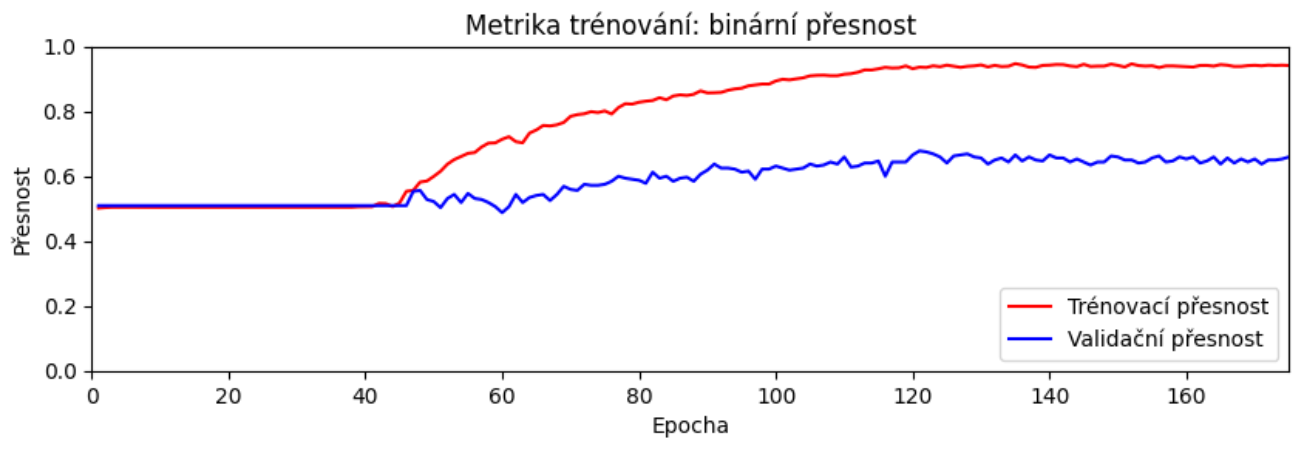
\includegraphics[width=1\textwidth]{Figures/EN_LSTM_binarni_presnost.png}
	\caption{Průběh trénování LSTM modelu v zobrazení metriky binární přesnosti}\label{fig:EN LSTM model train}
\end{figure}
\begin{lstlisting}[label=src:EN LSTM accuracy, caption={Výsledek LSTM modelu na anglickém datasetu po trénování~\ref{fig:EN LSTM model train}}]
	[Fáze 1] LSTM Přesnost:  0.609
	[Fáze 2] LSTM Přesnost:  0.633
\end{lstlisting}

Graf trénování~\ref{fig:EN LSTM GloVe model train} LSTM s technikou GloVe modelu a jeho následná přesnost~\ref{src:EN GloVe LSTM accuracy}.
\begin{figure}[H]
	\centering
	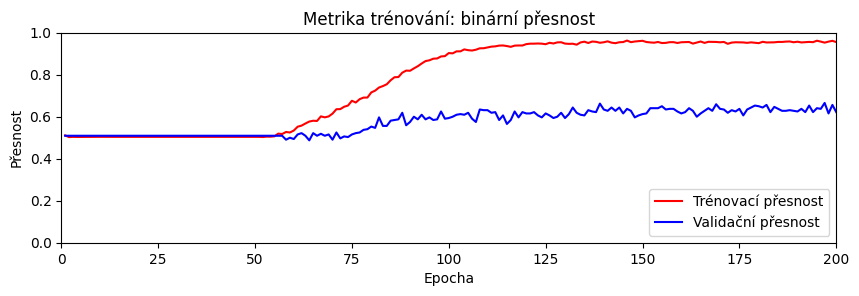
\includegraphics[width=1\textwidth]{Figures/EN_LSTM_GLOVE_binarni_presnost.png}
	\caption{Průběh trénování LSTM GloVe modelu v zobrazení metriky binární přesnosti}\label{fig:EN LSTM GloVe model train}
\end{figure}
\begin{lstlisting}[label=src:EN GloVe LSTM accuracy, caption={Výsledek GloVe LSTM modelu na anglickém datasetu po trénování~\ref{fig:EN LSTM GloVe model train}}]
	[Fáze 1] LSTM GloVe Přesnost:  0.582
	[Fáze 2] LSTM GloVe Přesnost:  0.615
\end{lstlisting}

Graf trénování~\ref{fig:EN LSTM Attention model train} LSTM s technikou Attention modelu a jeho následná přesnost~\ref{src:EN LSTM Attention accuracy}.
\begin{figure}[H]
	\centering
	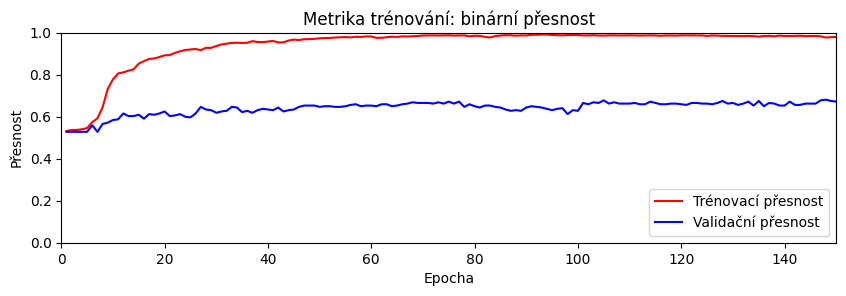
\includegraphics[width=1\textwidth]{Figures/EN_LSTM_Attention_binarni_presnost.png}
	\caption{Průběh trénování LSTM Attention modelu v zobrazení metriky binární přesnosti}\label{fig:EN LSTM Attention model train}
\end{figure}
\begin{lstlisting}[label=src:EN LSTM Attention accuracy, caption={Výsledek LSTM Attention modelu na anglickém datasetu po trénování~\ref{fig:EN LSTM Attention model train}}]
	[Fáze 1] LSTM Attention Přesnost:  0.631
	[Fáze 2] LSTM Attention Přesnost:  0.633
\end{lstlisting}

Graf trénování~\ref{fig:EN GRU model train} GRU modelu a jeho následná přesnost~\ref{src:EN GRU accuracy}.
\begin{figure}[H]
	\centering
	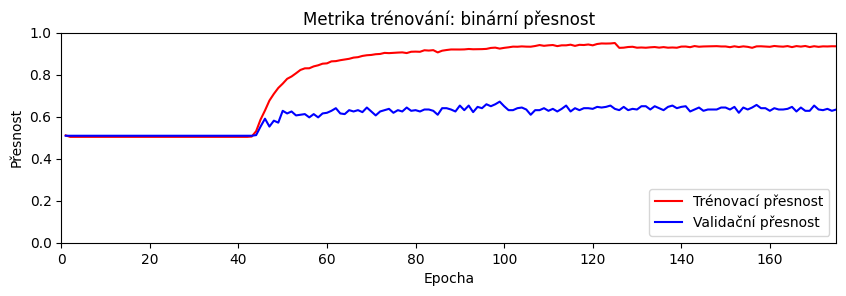
\includegraphics[width=1\textwidth]{Figures/EN_GRU_binarni_presnost.png}
	\caption{Průběh trénování GRU modelu v zobrazení metriky binární přesnosti}\label{fig:EN GRU model train}
\end{figure}
\begin{lstlisting}[label=src:EN GRU accuracy, caption={Výsledek GRU modelu na anglickém datasetu po trénování~\ref{fig:EN GRU model train}}]
	[Fáze 1] GRU Přesnost:  0.598
	[Fáze 2] GRU Přesnost:  0.606
\end{lstlisting}

Graf trénování~\ref{fig:EN GloVe GRU model train} GRU s technikou GloVe modelu a jeho následná přesnost~\ref{src:EN GloVe GRU accuracy}.
\begin{figure}[H]
	\centering
	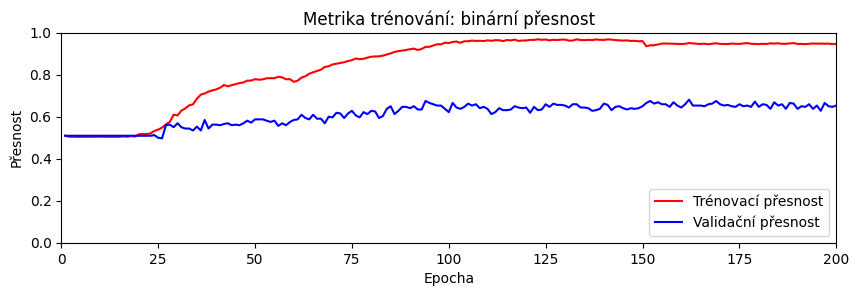
\includegraphics[width=1\textwidth]{Figures/EN_GRU_GLOVE_binarni_presnost.png}
	\caption{Průběh trénování GRU modelu s technikou GloVe v zobrazení metriky binární přesnosti}\label{fig:EN GloVe GRU model train}
\end{figure}
\begin{lstlisting}[label=src:EN GloVe GRU accuracy, caption={Výsledek GRU modelu s technikou GloVe na anglickém datasetu po trénování~\ref{fig:EN GloVe GRU model train}}]
	[Fáze 1] GRU GloVe Přesnost:  0.617
	[Fáze 2] GRU GloVe Přesnost:  0.647
\end{lstlisting}

Graf trénování~\ref{fig:EN Attention GRU model train} GRU s technikou Attention modelu a jeho následná přesnost~\ref{src:EN Attention GRU accuracy}.
\begin{figure}[H]
	\centering
	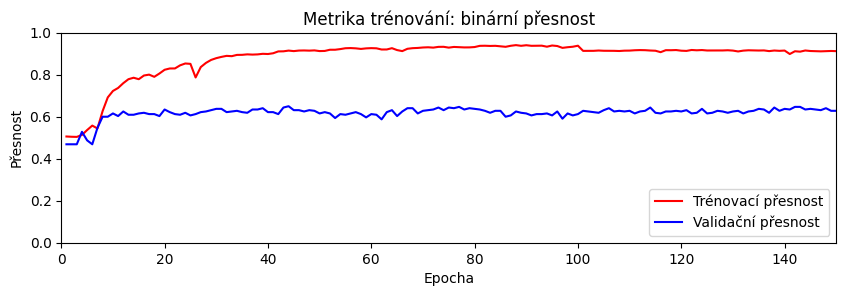
\includegraphics[width=1\textwidth]{Figures/EN_GRU_Attention_binarni_presnost.png}
	\caption{Průběh trénování GRU modelu s technikou Attention v zobrazení metriky binární přesnosti}\label{fig:EN Attention GRU model train}
\end{figure}
\begin{lstlisting}[label=src:EN Attention GRU accuracy, caption={Výsledek GRU modelu s technikou Attention na anglickém datasetu po trénování~\ref{fig:EN Attention GRU model train}}]
	[Fáze 1] GRU Attention Přesnost:  0.590
	[Fáze 2] GRU Attention Přesnost:  0.639
\end{lstlisting}

Graf trénování~\ref{fig:EN BERT model train} BERT modelu a jeho následná přesnost~\ref{src:EN BERT accuracy}.
\begin{figure}[H]
	\centering
	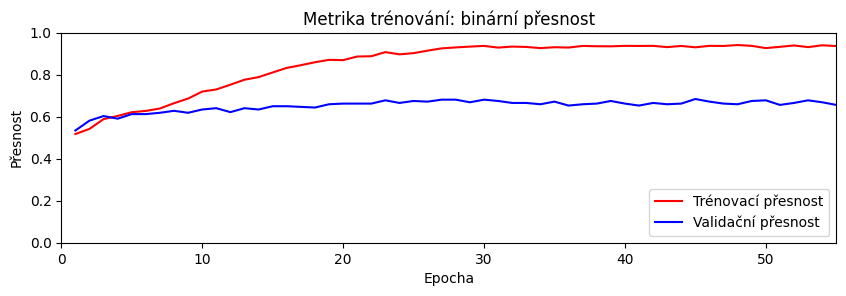
\includegraphics[width=1\textwidth]{Figures/EN_BERT_binarni_presnost.png}
	\caption{Průběh trénování BERT modelu v zobrazení metriky binární přesnosti}\label{fig:EN BERT model train}
\end{figure}
\begin{lstlisting}[label=src:EN BERT accuracy, caption={Výsledek BERT modelu na anglickém datasetu po trénování~\ref{fig:EN BERT model train}}]
	[Fáze 1] BERT Přesnost:  0.652
	[Fáze 2] BERT Přesnost:  0.660
\end{lstlisting}

Podle celkové tabulky~\ref{tab:EN trenovani klasifikatoru} dosáhl nejlepší přesnosti klasifikátor BERT.\@
Klasifikátory BERT, LSTM s technikou Attention a GRU s technikou Attention projevovaly schopnost učení již od brzkého začátku trénování na trénovacích datech.
Naopak klasifikátory LSTM, GRU, LSTM s technikou GloVe a GRU s technikou GloVe vykazovaly pomalé počáteční učení.
Každopádně u všech klasifikátorů se postupem času zlepšovala jak trénovací, tak validační přesnost, což naznačuje postupné zdokonalování modelu při učení.
\begin{table}[H]
	\centering
	\caption{Trénování klasifikátorů}\label{tab:EN trenovani klasifikatoru}
	\begin{tabular}{ c c c }
			\toprule
			Klasifikátor & dosažená přesnost v první fázi & dosažená přesnost ve druhé fázi\\
			\midrule
            LSTM & 61 \% & 63 \%\\
            LSTM s technikou GloVe & 58 \% & 62 \%\\
            LSTM s technikou Attention & 63 \% & 63 \%\\
            GRU & 60 \% & 61 \%\\
            GRU s technikou GloVe & 62 \% & 65 \%\\
            GRU s technikou Attention & 59 \% & 64 \%\\
            \textbf{BERT} & \textbf{65 \%} & \textbf{66 \%}\\
			\midrule
		\end{tabular}
\end{table}

\subsubsection{Počet trénovacích epoch}
Klasifikátory s použitím stejné techniky mají tendenci se učit podobným způsobem, což je patrné z tabulky epoch klasifikátorů~\ref{tab:EN pocet epoch}.
Klasifikátor BERT prošel nejméně učícími epochami ze všech ostatních klasifikátorů a dosáhl nejlepšího učení viz.~\ref{tab:EN trenovani klasifikatoru}.

\begin{table}[H]
	\centering
	\caption{Trénování klasifikátorů}\label{tab:EN pocet epoch}
	\begin{tabular}{ c c c }
			\toprule
			Klasifikátor & počet epoch první fáze & počet epoch druhé fázi\\
			\midrule
            LSTM & 125 & 50\\
            LSTM s technikou GloVe & 150 & 50\\
            LSTM s technikou Attention & 100 & 50\\
            GRU & 125 & 50\\
            GRU s technikou GloVe & 150 & 50\\
            GRU s technikou Attention & 100 & 50\\
            \textbf{BERT} & \textbf{50} & \textbf{50}\\
			\midrule
		\end{tabular}
\end{table}

\subsubsection{Doba trénování}
Průměrná doba trénování klasifikátorů~\ref{tab:EN doba trenovani} je přibližně 9 minut.
Je však třeba poznamenat, že klasifikátor BERT představuje výjimku, neboť i přes nejmenší počet učících epoch se trénoval nejdéle ze všech klasifikátorů, konkrétně 17 minut a 4 vteřiny.
Nejrychleji učícím se klasifikátorem je GRU s Attention technikou.

\begin{table}[H]
	\centering
	\caption{Doba trénování klasifikátorů}\label{tab:EN doba trenovani}
	\begin{tabular}{ c c c c }
			\toprule
			Klasifikátor & doba trénování první fáze & doba trénování druhé fázi & celková doba trénování\\
			\midrule
            LSTM & 373 s & 167 s & 541 s\\
            LSTM s technikou GloVe & 493 s & 168 s & 661 s\\
            LSTM s technikou Attention & 287 s & 138 s & 426 s\\
            GRU & 406 s & 160 s & 566 s\\
            GRU s technikou GloVe & 483 s & 161 s & 644 s\\
            \textbf{GRU s technikou Attention} & \textbf{268 s} & \textbf{127 s} & \textbf{396 s}\\
            BERT & 565 s & 459 s & 1024 s\\
			\midrule
		\end{tabular}
\end{table}

\subsubsection{Prioritizace predikce}
V následujících confusion maticích~\ref{fig:EN LSTM model conf}~\ref{fig:EN LSTM GloVe model conf}~\ref{fig:EN LSTM Attention model conf}~\ref{fig:EN GRU model conf}~\ref{fig:EN GRU GloVe model conf}~\ref{fig:EN GRU Attention model conf}~\ref{fig:EN BERT model conf} jsou zobrazeny predikce modelu ve čtyřech kategoriích: správně pozitivní (true positive), chybně pozitivní (false positive), chybně negativní (false negative) a správně negativní (true negative).
Ideálním scénářem je, když model dosahuje co nejvíce správně pozitivních a správně negativních předpovědí.
Jakákoli preference jedné z možných odpovědí (psáno člověkem nebo strojově přeložené) představuje chybné naučení modelu.
Cílem je dosáhnout vyváženého a správného předpovídání bez přehnaného zkreslení ve prospěch jedné kategorie.
Pouze takový model je schopný poskytovat spolehlivé výsledky a má skutečnou hodnotu při klasifikaci.

Graf confusion matice~\ref{fig:EN LSTM model conf} pro klasifikátor LSTM.\@
\begin{figure}[H]
	\centering
	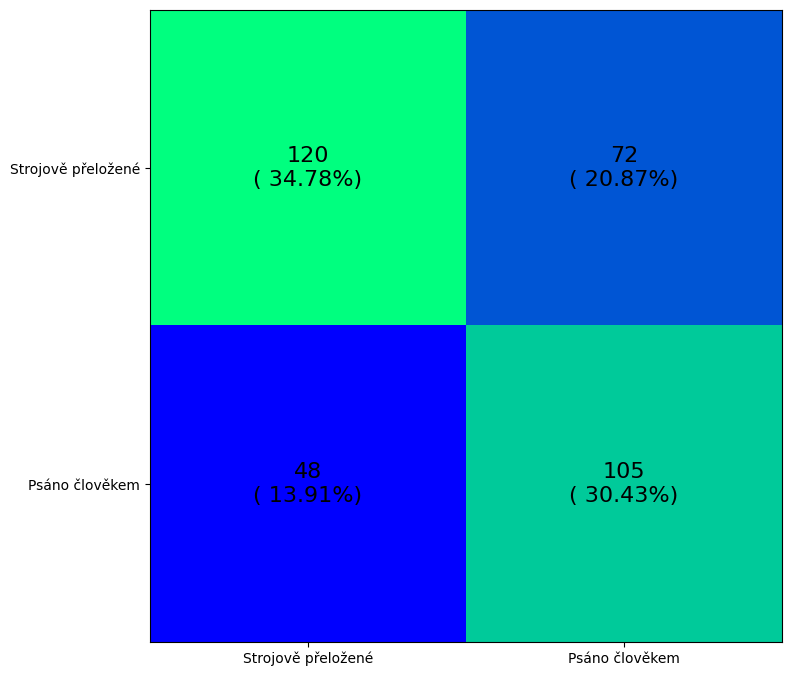
\includegraphics[width=0.6\textwidth]{Figures/EN_LSTM_conf.png}
	\caption{Výsledné predikování LSTM modelu na testovacích datech zobrazené v confusion matrix}\label{fig:EN LSTM model conf}
\end{figure}

Graf confusion matice~\ref{fig:EN LSTM GloVe model conf} pro klasifikátor LSTM s technikou GloVe.
\begin{figure}[H]
	\centering
	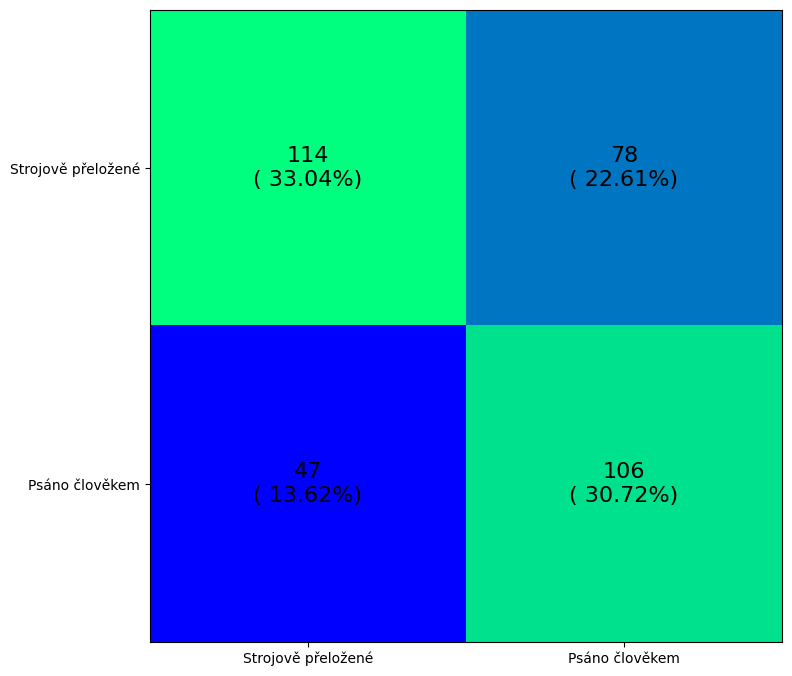
\includegraphics[width=0.6\textwidth]{Figures/EN_LSTM_GLOVE_conf.png}
	\caption{Výsledné predikování LSTM s technikou GloVe modelu na testovacích datech zobrazené v confusion matrix}\label{fig:EN LSTM GloVe model conf}
\end{figure}

Graf confusion matice~\ref{fig:EN LSTM Attention model conf} pro klasifikátor LSTM s technikou Attention.
\begin{figure}[H]
	\centering
	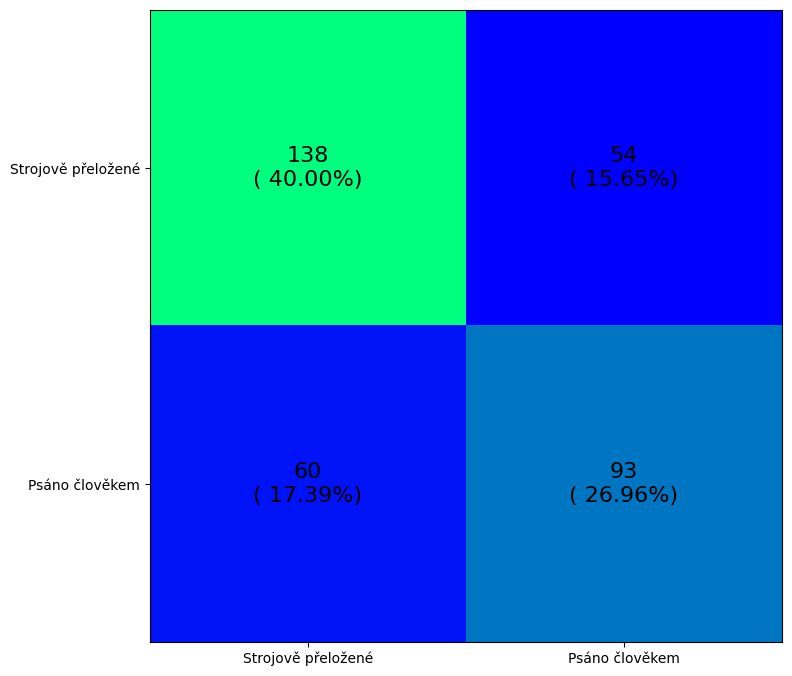
\includegraphics[width=0.6\textwidth]{Figures/EN_LSTM_Attention_conf.png}
	\caption{Výsledné predikování LSTM s technikou Attention modelu na testovacích datech zobrazené v confusion matrix}\label{fig:EN LSTM Attention model conf}
\end{figure}

Graf confusion matice~\ref{fig:EN GRU model conf} pro klasifikátor GRU.\@
\begin{figure}[H]
	\centering
	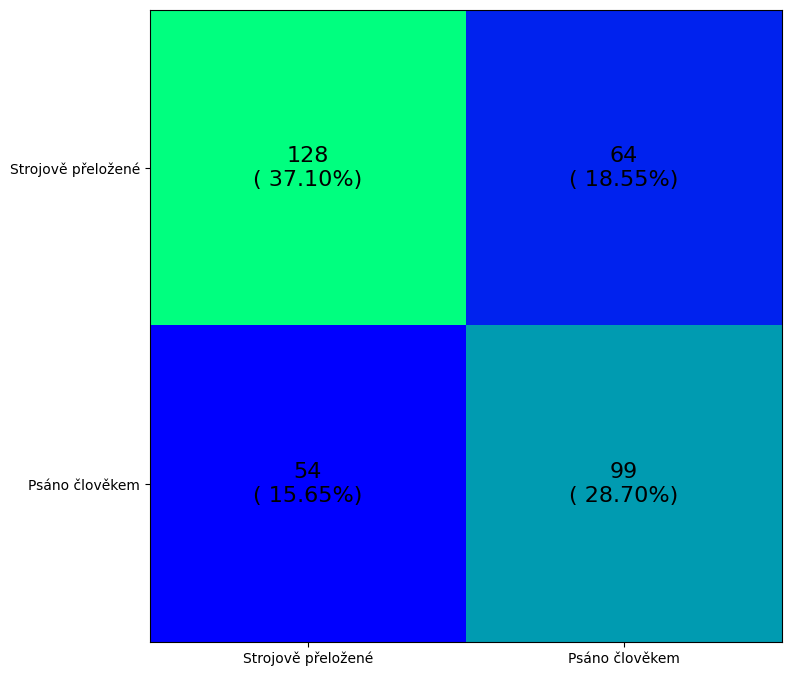
\includegraphics[width=0.6\textwidth]{Figures/EN_GRU_conf.png}
	\caption{Výsledné predikování GRU modelu na testovacích datech zobrazené v confusion matrix}\label{fig:EN GRU model conf}
\end{figure}

Graf confusion matice~\ref{fig:EN GRU GloVe model conf} pro klasifikátor GRU s technikou GloVe.
\begin{figure}[H]
	\centering
	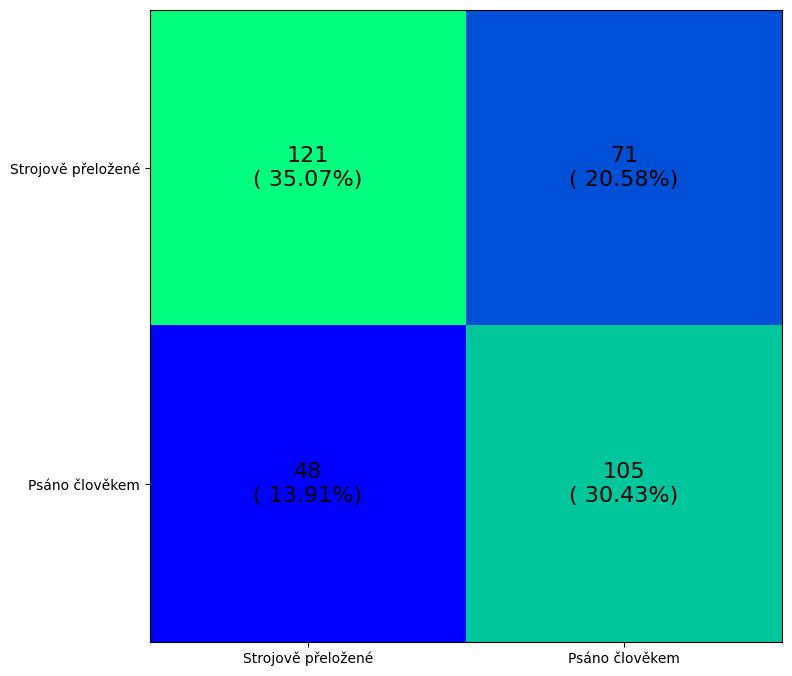
\includegraphics[width=0.6\textwidth]{Figures/EN_GRU_GLOVE_conf.png}
	\caption{Výsledné predikování GRU s technikou GloVe modelu na testovacích datech zobrazené v confusion matrix}\label{fig:EN GRU GloVe model conf}
\end{figure}

Graf confusion matice~\ref{fig:EN GRU Attention model conf} pro klasifikátor GRU s technikou Attention.
\begin{figure}[H]
	\centering
	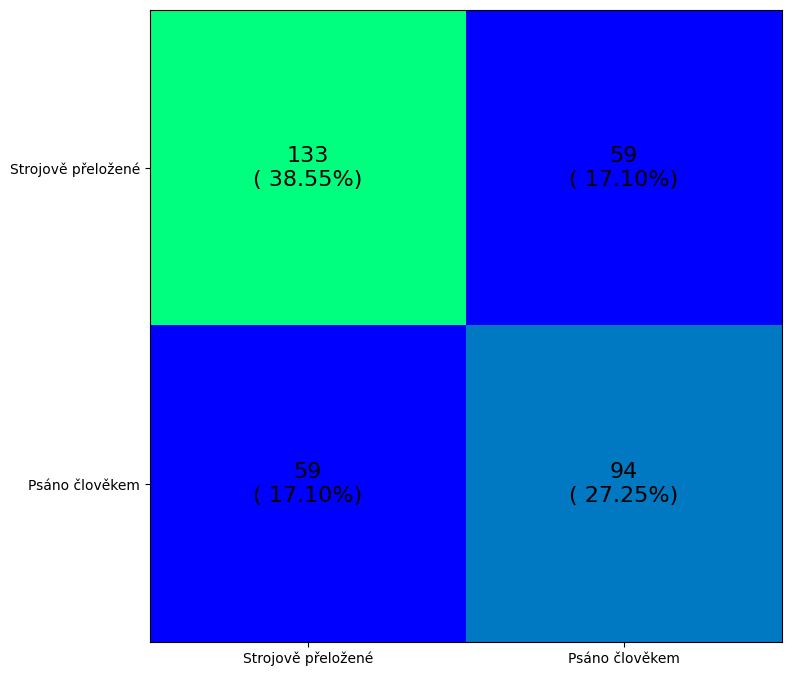
\includegraphics[width=0.6\textwidth]{Figures/EN_GRU_Attention_conf.png}
	\caption{Výsledné predikování GRU s technikou Attention modelu na testovacích datech zobrazené v confusion matrix}\label{fig:EN GRU Attention model conf}
\end{figure}

Graf confusion matice~\ref{fig:EN BERT model conf} pro klasifikátor BERT.\@
\begin{figure}[H]
	\centering
	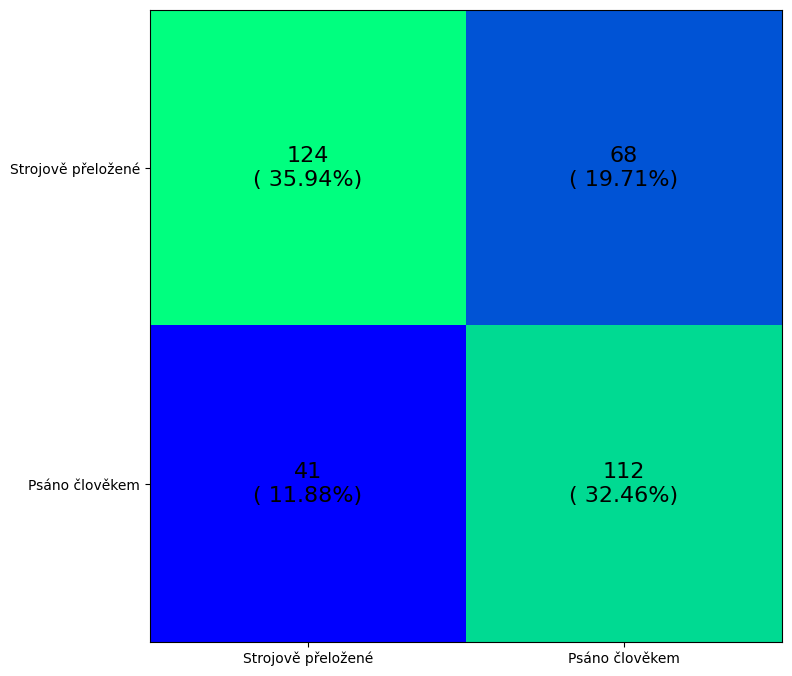
\includegraphics[width=0.6\textwidth]{Figures/EN_BERT_conf.png}
	\caption{Výsledné predikování BERT modelu na testovacích datech zobrazené v confusion matrix}\label{fig:EN BERT model conf}
\end{figure}

Většina klasifikátorů předpovídá vyváženě jak pro detekci strojově přeložených, tak i člověkem psaných vět.
Nicméně klasifikátor GRU s technikou GloVe se od ostatních klasifikátorů liší a vykazuje větší tendenci k predikci vět psaných člověkem.

\subsubsection{Predikce na reálných datech}
Pro reálná data byla vybrána věta `I am a very smart robot writting the message'.
V následující tabulce~\ref{tab:EN predikce} jsou uvedeny predikce jednotlivých klasifikátorů.
Jelikož tato věta byla psána autorem práce, správnou predikcí je `psáno člověkem'.

\begin{table}[H]
	\centering
	\caption{Predikce na reálné větě}\label{tab:EN predikce}
	\begin{tabular}{ c c c }
			\toprule
			Klasifikátor & predikční skóre & interpretace skóre\\
			\midrule
            \textbf{LSTM} & \textbf{0.98337} & \textbf{Psáno člověkem}\\
            LSTM s technikou GloVe & 0.01706 & Strojově přeloženo\\
            \textbf{LSTM s technikou Attention} & \textbf{0.99378} & \textbf{Psáno člověkem}\\
            GRU & 0.07115 & Strojově přeloženo\\
            \textbf{GRU s technikou GloVe} & \textbf{0.99479} & \textbf{Psáno člověkem}\\
            \textbf{GRU s technikou Attention} & \textbf{0.92976} & \textbf{Psáno člověkem}\\
            BERT & 0.00019 & Strojově přeloženo\\
			\midrule
		\end{tabular}
\end{table}

Pouze klasifikátory LSTM, LSTM s technikou attention, GRU s technikou GloVe a GRU s technikou Attention byly schopny správně predikovat odpověď.

\section{Výsledné klasifikátory více jazyčného datasetu}
Klasifikátory, určené pro anglická a vícejazyčná data, sdílí podobné architektury a využívají podobné techniky a strukturu sítě.
Tento přístup, kdy jsou osvědčené architektury a techniky aplikovány na různá jazyková prostředí s minimálními úpravami, je často praktikován.
Tím je umožněno využít předchozích znalostí a zkušeností s architekturou a přenést je na nová jazyková prostředí.
Tímto způsobem je dosaženo efektivního využití existujících modelů a minimalizace potřeby vytvářet nové architektury pro každý jazyk zvlášť.

\subsection{Architektura klasifikátoru LSTM}
Tento klasifikátor~\ref{tab:MULTI LSTM model} je identický svému anglickému protějšku~\ref{arch: LSTM}, s výjimkou počtu parametrů.
Celkový počet parametrů modelu činí 5 861 761.

\begin{table}[H]
	\centering
	\caption{Více jazyčný LSTM model}\label{tab:MULTI LSTM model}
	\begin{tabular}{ c c c }
			\toprule
			Vrstva modelu & výstupný formát dat & počet parametrů\\
			\midrule
            TextVectorization & (None, 256) & 0\\         
            Embedding & (None, 256, 128) & 5 120 000\\   
            Bidirectional & (None, 256, 256) & 263 168\\    
            Bidirectional & (None, 256) & 394 240\\
			Dense & (None, 256) & 65 792\\ 
			Gaussian Noise & (None, 256) & 0\\
            Dense & (None, 64) & 16 448\\ 
			Gaussian Noise & (None, 64) & 0\\
			Dense & (None, 32) & 2 080\\ 
            Dropout & (None, 32) & 0\\   
            Dense & (None, 1) & 33\\ 
			\midrule
		\end{tabular}
\end{table}

\subsection{Architektura klasifikátoru GRU}
Tento klasifikátor~\ref{tab:MULTI GRU model} je identický svému anglickému protějšku~\ref{arch: GRU}, s výjimkou počtu parametrů.
Celkový počet parametrů modelu činí 5 698 945.

\begin{table}[H]
	\centering
	\caption{Více jazyčný GRU model}\label{tab:MULTI GRU model}
	\begin{tabular}{ c c c }
			\toprule
			Vrstva modelu & výstupný formát dat & počet parametrů\\
			\midrule
            TextVectorization & (None, 256) & 0\\         
            Embedding & (None, 256, 128) & 5 120 000\\   
            Bidirectional & (None, 256, 256) & 198 144\\    
            Bidirectional & (None, 256) & 296 448\\
			Dense & (None, 256) & 65 792\\ 
			Gaussian Noise & (None, 256) & 0\\
            Dense & (None, 64) & 16 448\\ 
			Gaussian Noise & (None, 64) & 0\\
			Dense & (None, 32) & 2 080\\ 
            Dropout & (None, 32) & 0\\   
            Dense & (None, 1) & 33\\ 
			\midrule
		\end{tabular}
\end{table}

\subsection{Architektura klasifikátoru LSTM s technikou GloVe}
Tento klasifikátor~\ref{tab:MULTI LSTM GloVe model} je identický svému anglickému protějšku~\ref{arch: LSTM GloVe}, s výjimkou počtu parametrů.
Celkový počet parametrů modelu činí 8 815 889.

\begin{table}[H]
	\centering
	\caption{Více jazyčný LSTM model s technikou GloVe}\label{tab:MULTI LSTM GloVe model}
	\begin{tabular}{ c c c }
			\toprule
			Vrstva modelu & výstupný formát dat & počet parametrů\\
			\midrule
            TextVectorization & (None, 256) & 0\\         
            GloVe & (None, 256, 200) & 8 000 400\\   
            Bidirectional & (None, 256, 256) & 336 896\\    
            Bidirectional & (None, 256) & 394 240\\
			Dense & (None, 256) & 65 792\\ 
			Gaussian Noise & (None, 256) & 0\\
            Dense & (None, 64) & 16 448\\ 
			Gaussian Noise & (None, 64) & 0\\
			Dense & (None, 32) & 2 080\\ 
			Gaussian Noise & (None, 32) & 0\\
            Dropout & (None, 32) & 0\\   
            Dense & (None, 1) & 33\\ 
			\midrule
		\end{tabular}
\end{table}


\subsection{Architektura klasifikátoru GRU s technikou GloVe}
Tento klasifikátor~\ref{tab:MULTI GRU GloVe model} je identický svému anglickému protějšku~\ref{arch: GRU GloVe}, s výjimkou počtu parametrů.
Celkový počet parametrů modelu činí 8 634 641.

\begin{table}[H]
	\centering
	\caption{Více jazyčný GRU model s technikou GloVe}\label{tab:MULTI GRU GloVe model}
	\begin{tabular}{ c c c }
			\toprule
			Vrstva modelu & výstupný formát dat & počet parametrů\\
			\midrule
            TextVectorization & (None, 256) & 0\\         
            GloVe & (None, 256, 200) & 8 000 400\\   
            Bidirectional & (None, 256, 256) & 336 896\\    
            Bidirectional & (None, 256) & 394 240\\
			Dense & (None, 256) & 65 792\\ 
			Gaussian Noise & (None, 256) & 0\\
            Dense & (None, 64) & 16 448\\ 
			Gaussian Noise & (None, 64) & 0\\
			Dense & (None, 32) & 2 080\\ 
			Gaussian Noise & (None, 32) & 0\\
            Dropout & (None, 32) & 0\\   
            Dense & (None, 1) & 33\\ 
			\midrule
		\end{tabular}
\end{table}

\subsection{Architektura klasifikátoru LSTM s technikou Attention}
Tento klasifikátor~\ref{tab:MULTI LSTM Attention model} je identický svému anglickému protějšku~\ref{arch: LSTM Attention}, s výjimkou počtu parametrů.
Celkový počet parametrů modelu nyní činí 5 862 273.

\begin{table}[H]
	\centering
	\caption{Více jazyčný LSTM model s technikou Attention}\label{tab:MULTI LSTM Attention model}
	\begin{tabular}{ c c c }
			\toprule
			Vrstva modelu & výstupný formát dat & počet parametrů\\
			\midrule
            Text Vectorization & (None, 256) & 0\\         
            Embedding & (None, 256, 128) & 5 120 000\\   
            Bidirectional & (None, 256, 256) & 263 168\\    
			Gaussian Noise & (None, 256, 256) & 0\\
            Bidirectional & (None, 256, 256) & 394 240\\
			Gaussian Noise & (None, 256, 256) & 0\\
			Attention & (None, 256) & 512\\
            Dense & (None, 256) & 65 792\\ 
			Gaussian Noise & (None, 256) & 0\\
			Dense & (None, 64) & 16 448\\ 
			Gaussian Noise & (None, 64) & 0\\
			Dense & (None, 32) & 2 080\\ 
			Gaussian Noise & (None, 32) & 0\\
            Dropout & (None, 32) & 0\\   
            Dense & (None, 1) & 33\\ 
			\midrule
		\end{tabular}
\end{table}

\subsection{Architektura klasifikátoru GRU s technikou Attention}
Tento klasifikátor~\ref{tab:MULTI GRU Attention model} je identický svému anglickému protějšku~\ref{arch: GRU Attention}, s výjimkou počtu parametrů.
Celkový počet parametrů modelu nyní činí 5 699 457.

\begin{table}[H]
	\centering
	\caption{Více jazyčný GRU model s technikou Attention}\label{tab:MULTI GRU Attention model}
	\begin{tabular}{ c c c }
			\toprule
			Vrstva modelu & výstupný formát dat & počet parametrů\\
			\midrule
            Text Vectorization & (None, 256) & 0\\         
            Embedding & (None, 256, 128) & 5 120 000\\   
            Bidirectional & (None, 256, 256) & 198 144\\    
			Gaussian Noise & (None, 256, 256) & 0\\
            Bidirectional & (None, 256, 256) & 296 448\\
			Gaussian Noise & (None, 256, 256) & 0\\
			Attention & (None, 256) & 512\\
            Dense & (None, 256) & 65 792\\ 
			Gaussian Noise & (None, 256) & 0\\
			Dense & (None, 64) & 16 448\\ 
			Gaussian Noise & (None, 64) & 0\\
			Dense & (None, 32) & 2 080\\ 
			Gaussian Noise & (None, 32) & 0\\
            Dropout & (None, 32) & 0\\   
            Dense & (None, 1) & 33\\ 
			\midrule
		\end{tabular}
\end{table}


\subsection{Architektura klasifikátoru BERT}
Tento klasifikátor~\ref{tab:MULTI BERT model} je identický svému anglickému protějšku~\ref{arch: BERT}.
Celkový počet parametrů modelu činí 28 764 162.

\begin{table}[H]
	\centering
	\caption{Více jazyčný BERT model}\label{tab:MULTI BERT model}
	\begin{tabular}{ c c c }
			\toprule
			Vrstva modelu & výstupný formát dat & počet parametrů\\
			\midrule
            InputLayer & (None,) & 0\\         
            Preprocessing & --- & 0\\   
            BERT encoder & --- & 28,763,649\\    
            Dropout & (None, 512) & 0\\  
            Dense & (None, 1) & 513\\ 
			\midrule
		\end{tabular}
\end{table}

\subsection{Výsledky klasifikátorů}
\subsubsection{Trénovací fáze}
V následujících grafech~\ref{fig:MULTI LSTM model train}~\ref{fig:MULTI LSTM GloVe model train}~\ref{fig:MULTI LSTM Attention model train}~\ref{fig:MULTI GRU model train}~\ref{fig:MULTI GloVe GRU model train}~\ref{fig:MULTI Attention GRU model train}~\ref{fig:MULTI BERT model train} jsou znázorněny křivky učení v průběhu postupně vykonávaných epoch.
Červená křivka představuje přesnost predikce modelu na trénovacích datech a modrá křivka představuje přesnost predikce modelu na validačních datech.

Graf trénování~\ref{fig:MULTI LSTM model train} LSTM modelu a jeho následná přesnost~\ref{src:MULTI LSTM accuracy}.
\begin{figure}[H]
	\centering
	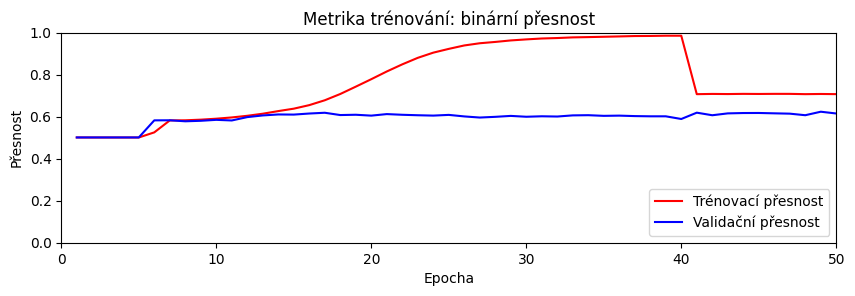
\includegraphics[width=1\textwidth]{Figures/MULTI_LSTM_binarni_presnost.png}
	\caption{Průběh trénování LSTM modelu v zobrazení metriky binární přesnosti}\label{fig:MULTI LSTM model train}
\end{figure}
\begin{lstlisting}[label=src:MULTI LSTM accuracy, caption={Výsledek LSTM modelu na více jazyčném datasetu po trénování~\ref{fig:MULTI LSTM model train}}]
	[Fáze 1] LSTM Přesnost:  0.606
	[Fáze 2] LSTM Přesnost:  0.606
\end{lstlisting}

Graf trénování~\ref{fig:MULTI LSTM GloVe model train} LSTM s technikou GloVe modelu a jeho následná přesnost~\ref{src:MULTI GloVe LSTM accuracy}.
\begin{figure}[H]
	\centering
	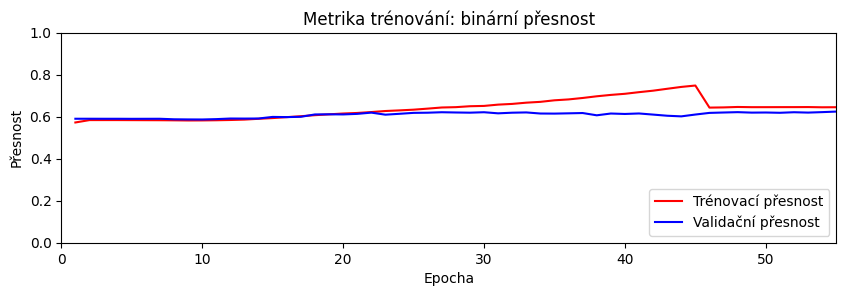
\includegraphics[width=1\textwidth]{Figures/MULTI_LSTM_GLOVE_binarni_presnost.png}
	\caption{Průběh trénování LSTM GloVe modelu v zobrazení metriky binární přesnosti}\label{fig:MULTI LSTM GloVe model train}
\end{figure}
\begin{lstlisting}[label=src:MULTI GloVe LSTM accuracy, caption={Výsledek GloVe LSTM modelu na více jazyčném datasetu po trénování~\ref{fig:MULTI LSTM GloVe model train}}]
	[Fáze 1] LSTM GloVe Přesnost:  0.612
	[Fáze 2] LSTM GloVe Přesnost:  0.612
\end{lstlisting}

Graf trénování~\ref{fig:MULTI LSTM Attention model train} LSTM s technikou Attention modelu a jeho následná přesnost~\ref{src:MULTI LSTM Attention accuracy}.
\begin{figure}[H]
	\centering
	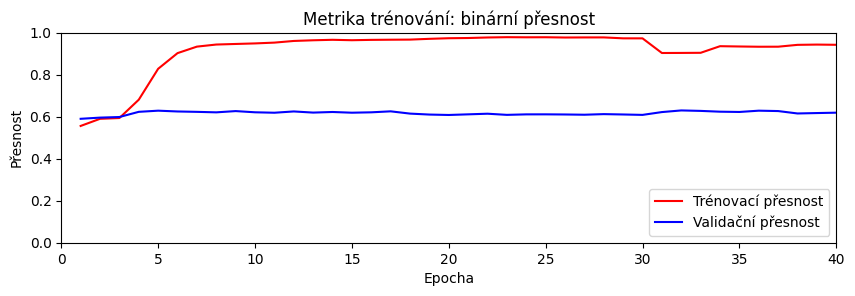
\includegraphics[width=1\textwidth]{Figures/MULTI_LSTM_Attention_binarni_presnost.png}
	\caption{Průběh trénování LSTM Attention modelu v zobrazení metriky binární přesnosti}\label{fig:MULTI LSTM Attention model train}
\end{figure}
\begin{lstlisting}[label=src:MULTI LSTM Attention accuracy, caption={Výsledek LSTM Attention modelu na více jazyčném datasetu po trénování~\ref{fig:MULTI LSTM Attention model train}}]
	[Fáze 1] LSTM Attention Přesnost:  0.597
	[Fáze 2] LSTM Attention Přesnost:  0.600
\end{lstlisting}

Graf trénování~\ref{fig:MULTI GRU model train} GRU modelu a jeho následná přesnost~\ref{src:MULTI GRU accuracy}.
\begin{figure}[H]
	\centering
	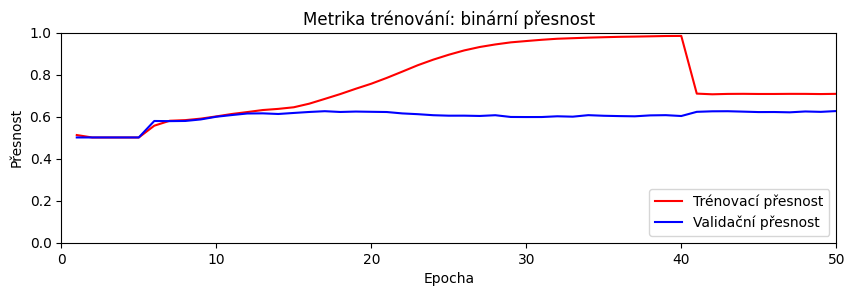
\includegraphics[width=1\textwidth]{Figures/MULTI_GRU_binarni_presnost.png}
	\caption{Průběh trénování GRU modelu v zobrazení metriky binární přesnosti}\label{fig:MULTI GRU model train}
\end{figure}
\begin{lstlisting}[label=src:MULTI GRU accuracy, caption={Výsledek GRU modelu na více jazyčném datasetu po trénování~\ref{fig:MULTI GRU model train}}]
	[Fáze 1] GRU Přesnost:  0.611
	[Fáze 2] GRU Přesnost:  0.611
\end{lstlisting}

Graf trénování~\ref{fig:MULTI GloVe GRU model train} GRU s technikou GloVe modelu a jeho následná přesnost~\ref{src:MULTI GloVe GRU accuracy}.
\begin{figure}[H]
	\centering
	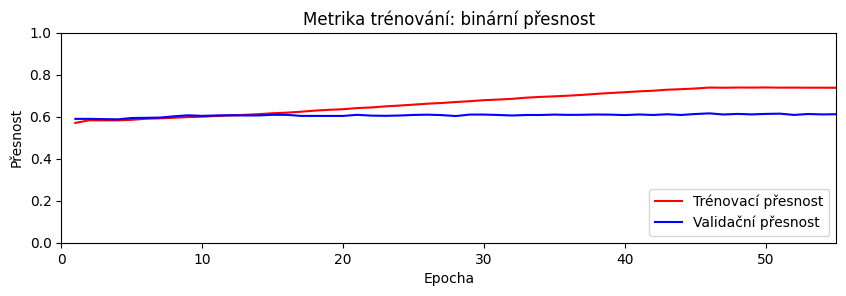
\includegraphics[width=1\textwidth]{Figures/MULTI_GRU_GLOVE_binarni_presnost.png}
	\caption{Průběh trénování GRU s technikou GloVe modelu v zobrazení metriky binární přesnosti}\label{fig:MULTI GloVe GRU model train}
\end{figure}
\begin{lstlisting}[label=src:MULTI GloVe GRU accuracy, caption={Výsledek GRU s technikou GloVe modelu na více jazyčném datasetu po trénování~\ref{fig:MULTI GloVe GRU model train}}]
	[Fáze 1] GRU GloVe Přesnost:  0.595
	[Fáze 2] GRU GloVe Přesnost:  0.595
\end{lstlisting}

Graf trénování~\ref{fig:MULTI Attention GRU model train} GRU s technikou Attention modelu a jeho následná přesnost~\ref{src:MULTI Attention GRU accuracy}.
\begin{figure}[H]
	\centering
	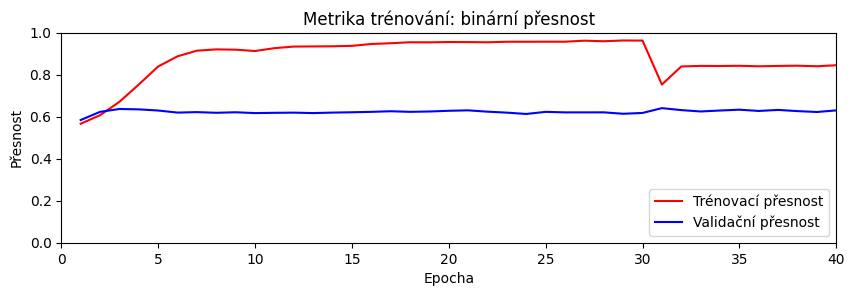
\includegraphics[width=1\textwidth]{Figures/MULTI_GRU_Attention_binarni_presnost.png}
	\caption{Průběh trénování GRU modelu s technikou Attention v zobrazení metriky binární přesnosti}\label{fig:MULTI Attention GRU model train}
\end{figure}
\begin{lstlisting}[label=src:MULTI Attention GRU accuracy, caption={Výsledek GRU modelu s technikou Attention na více jazyčném datasetu po trénování~\ref{fig:MULTI Attention GRU model train}}]
	[Fáze 1] GRU Attention Přesnost:  0.628
	[Fáze 2] GRU Attention Přesnost:  0.630
\end{lstlisting}

Graf trénování~\ref{fig:MULTI BERT model train} BERT modelu a jeho následná přesnost~\ref{src:MULTI BERT accuracy}.
\begin{figure}[H]
	\centering
	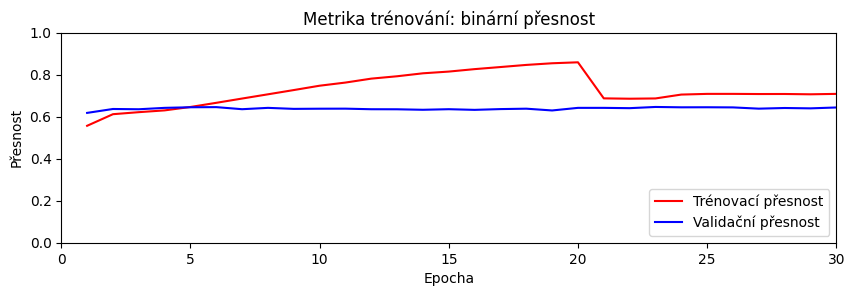
\includegraphics[width=1\textwidth]{Figures/MULTI_BERT_binarni_presnost.png}
	\caption{Průběh trénování BERT modelu v zobrazení metriky binární přesnosti}\label{fig:MULTI BERT model train}
\end{figure}
\begin{lstlisting}[label=src:MULTI BERT accuracy, caption={Výsledek BERT modelu na více jazyčném datasetu po trénování~\ref{fig:MULTI BERT model train}}]
	[Fáze 1] BERT Přesnost:  0.626
	[Fáze 2] BERT Přesnost:  0.627
\end{lstlisting}

Podle celkové tabulky~\ref{tab:MULTI trenovani klasifikatoru} dosáhly nejlepší přesnosti klasifikátory BERT a klasifikátor GRU s technikou Attention.
Klasifikátory LSTM a GRU vykazovaly pomalé počáteční učení, zatímco ostatní klasifikátory se rychleji naučily.
U většiny klasifikátorů se druhá fáze učení neprojevila jako výrazné zlepšení, s výjimkou klasifikátorů BERT, LSTM s technikou Attention a GRU s technikou Attention, které dosáhly lepší konfigurace modelu.

Grafy ukazují výrazné skoky ve trénovací přesnosti, což je způsobeno zahájením druhé fáze učení, kdy je vybrána nejlepší konfigurace na základě přesnosti na validačních datech.
Tyto skoky signalizují výběr konfigurace z počátku trénování, kdy byla hodnota trénovací přesnosti ještě nízká.
V tomto případě lze pozorovat, jak druhá fáze učení eliminuje přeučení na trénovacích datech.
\begin{table}[H]
	\centering
	\caption{Trénování klasifikátorů}\label{tab:MULTI trenovani klasifikatoru}
	\begin{tabular}{ c c c }
			\toprule
			Klasifikátor & dosažená přesnost v první fázi & dosažená přesnost ve druhé fázi\\
			\midrule
            LSTM & 61 \% & 61 \%\\
            LSTM s technikou GloVe & 61 \% & 61 \%\\
            LSTM s technikou Attention & 60 \% & 60 \%\\
            GRU & 61 \% & 61 \%\\
            GRU s technikou GloVe & 60 \% & 60 \%\\
            \textbf{GRU s technikou Attention} & \textbf{63} \% & \textbf{63} \%\\
            \textbf{BERT} & \textbf{63 \%} & \textbf{63 \%}\\
			\midrule
		\end{tabular}
\end{table}

\subsubsection{Počet trénovacích epoch}
Podle tabulky epoch klasifikátorů~\ref{tab:MULTI pocet epoch} je patrné, že klasifikátory využívající stejnou techniku vykazují tendenci učit se podobným způsobem.
Klasifikátor BERT prošel nejméně epochami z celé sady a dosáhl vyšší přesnosti než průměr mezi ostatními klasifikátory.

\begin{table}[H]
	\centering
	\caption{Trénování klasifikátorů}\label{tab:MULTI pocet epoch}
	\begin{tabular}{ c c c }
			\toprule
			Klasifikátor & počet epoch první fáze & počet epoch druhé fázi\\
			\midrule
			LSTM & 40 & 10\\
			LSTM s technikou GloVe & 45 & 10\\
			LSTM s technikou Attention & 30 & 10\\
			GRU & 40 & 10\\
			GRU s technikou GloVe & 45 & 10\\
			GRU s technikou Attention & 30 & 10\\
			\textbf{BERT} & \textbf{20} & \textbf{10}\\
			\midrule
		\end{tabular}
\end{table}

\subsubsection{Doba trénování}
Průměrná doba trénování klasifikátorů~\ref{tab:MULTI doba trenovani} je přibližně 14 minut.
Je však třeba poznamenat, že klasifikátor BERT představuje výjimku, neboť i přes nejmenší počet učících epoch se trénoval nejdéle ze všech klasifikátorů, konkrétně 2 hodiny 30 minut a 49 vteřin.
Nejrychleji učící se klasifikátory jsou LSTM s Attention technikou a GRU s Attention technikou.

\begin{table}[H]
	\centering
	\caption{Doba trénování klasifikátorů}\label{tab:MULTI doba trenovani}
	\begin{tabular}{ c c c c }
			\toprule
			Klasifikátor & doba trénování první fáze & doba trénování druhé fázi & celková doba trénování\\
			\midrule
			LSTM & 685 s & 166 s & 851 s\\
			LSTM s technikou GloVe & 745 s & 161 s & 907 s\\
			\textbf{LSTM s technikou Attention} & \textbf{592 s} & \textbf{189 s} & \textbf{781 s}\\
			GRU & 660 s & 155 s & 816 s\\
			GRU s technikou GloVe & 774 s & 163 s & 937 s\\
			\textbf{GRU s technikou Attention} & \textbf{584 s} & \textbf{196 s} & \textbf{780 s}\\
			BERT & 6032 s & 3017 s & 9049 s\\
			\midrule
		\end{tabular}
\end{table}

\subsubsection{Prioritizace predikce}
V následujících confusion maticích~\ref{fig:MULTI LSTM model conf}~\ref{fig:MULTI LSTM GloVe model conf}~\ref{fig:MULTI LSTM Attention model conf}~\ref{fig:MULTI GRU model conf}~\ref{fig:MULTI GRU GloVe model conf}~\ref{fig:MULTI GRU Attention model conf}~\ref{fig:MULTI BERT model conf} jsou zobrazeny predikce modelu ve čtyřech kategoriích: správně pozitivní (true positive), chybně pozitivní (false positive), chybně negativní (false negative) a správně negativní (true negative).
Ideálním scénářem je, když model dosahuje co nejvíce správně pozitivních a správně negativních předpovědí.
Jakákoli preference jedné z možných odpovědí (psáno člověkem nebo strojově přeložené) představuje chybné naučení modelu.
Cílem je dosáhnout vyváženého a správného předpovídání bez přehnaného zkreslení ve prospěch jedné kategorie.
Pouze takový model je schopný poskytovat spolehlivé výsledky a má skutečnou hodnotu při klasifikaci.

Graf confusion matice~\ref{fig:MULTI LSTM model conf} pro klasifikátor LSTM.\@
\begin{figure}[H]
	\centering
	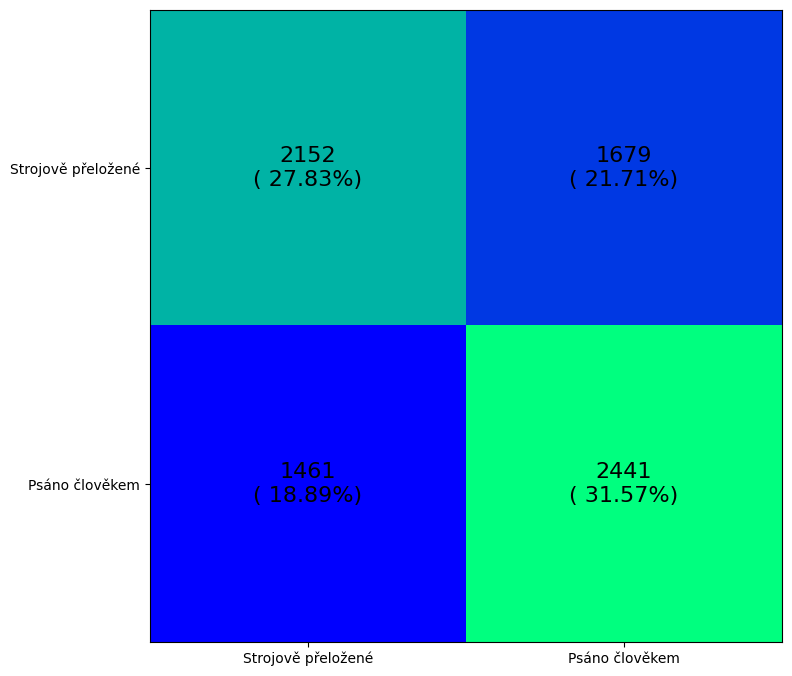
\includegraphics[width=0.6\textwidth]{Figures/MULTI_LSTM_conf.png}
	\caption{Výsledné predikování LSTM modelu na testovacích datech zobrazené v confusion matrix}\label{fig:MULTI LSTM model conf}
\end{figure}

Graf confusion matice~\ref{fig:MULTI LSTM GloVe model conf} pro klasifikátor LSTM s technikou GloVe.
\begin{figure}[H]
	\centering
	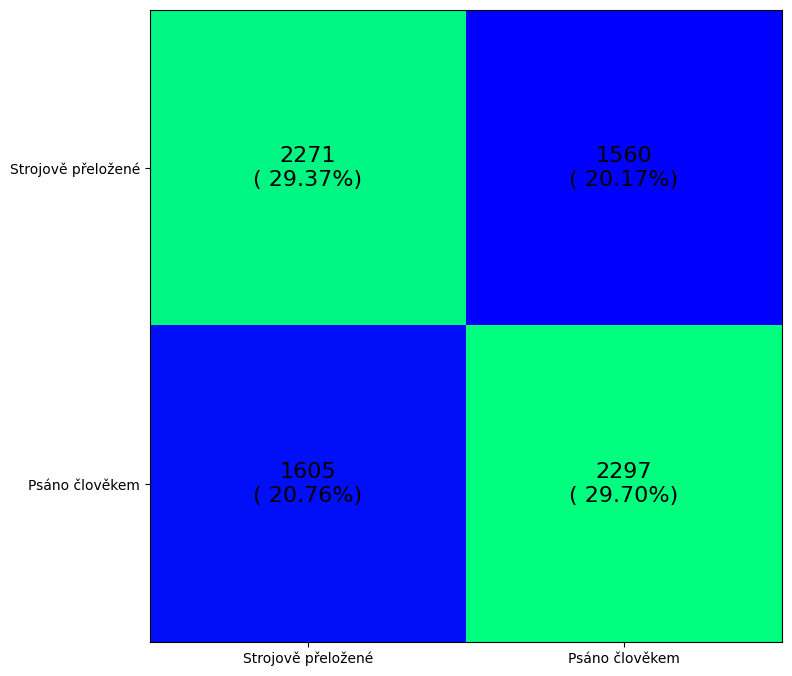
\includegraphics[width=0.6\textwidth]{Figures/MULTI_LSTM_GLOVE_conf.png}
	\caption{Výsledné predikování LSTM s technikou GloVe modelu na testovacích datech zobrazené v confusion matrix}\label{fig:MULTI LSTM GloVe model conf}
\end{figure}

Graf confusion matice~\ref{fig:MULTI LSTM Attention model conf} pro klasifikátor LSTM s technikou Attention.
\begin{figure}[H]
	\centering
	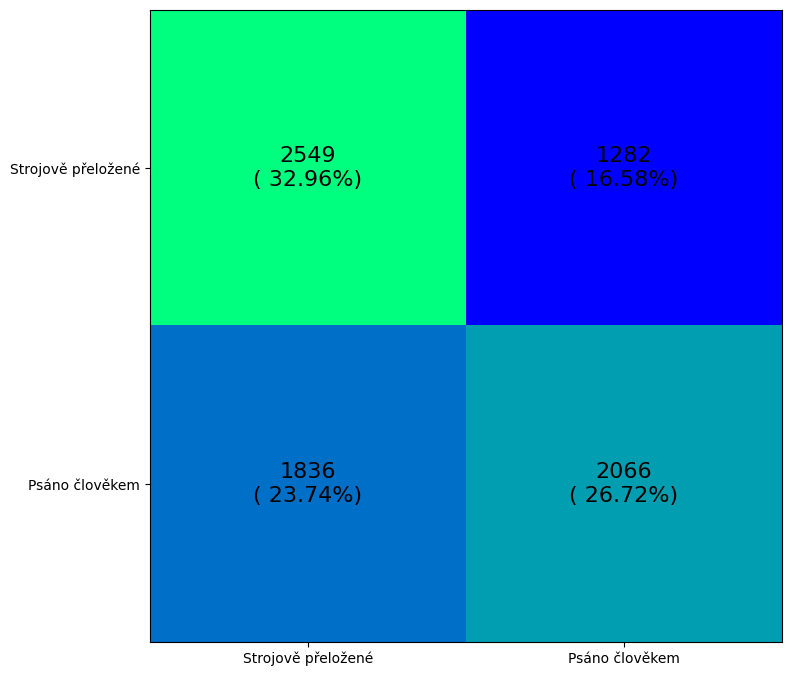
\includegraphics[width=0.6\textwidth]{Figures/MULTI_LSTM_Attention_conf.png}
	\caption{Výsledné predikování LSTM s technikou Attention modelu na testovacích datech zobrazené v confusion matrix}\label{fig:MULTI LSTM Attention model conf}
\end{figure}

Graf confusion matice~\ref{fig:MULTI GRU model conf} pro klasifikátor GRU.\@
\begin{figure}[H]
	\centering
	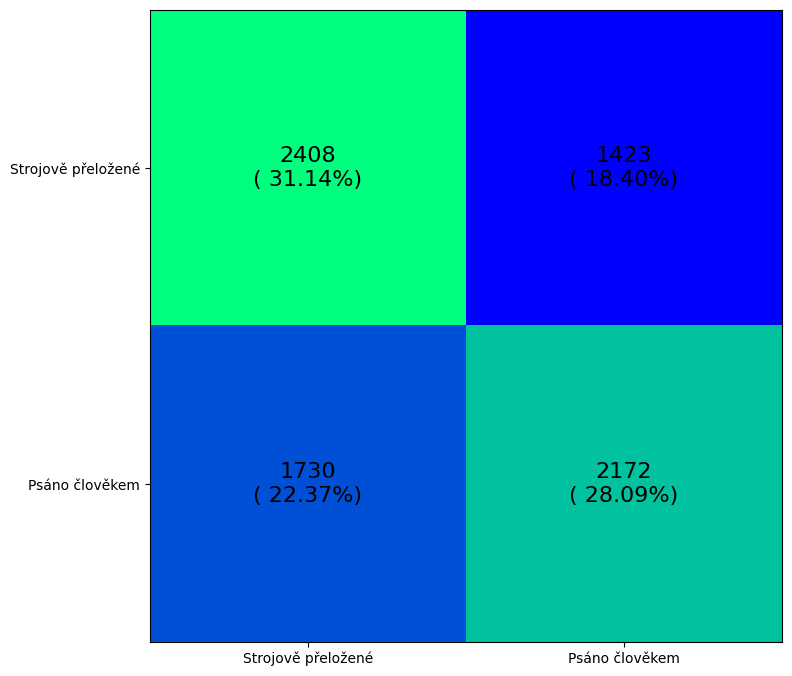
\includegraphics[width=0.6\textwidth]{Figures/MULTI_GRU_conf.png}
	\caption{Výsledné predikování GRU modelu na testovacích datech zobrazené v confusion matrix}\label{fig:MULTI GRU model conf}
\end{figure}

Graf confusion matice~\ref{fig:MULTI GRU GloVe model conf} pro klasifikátor GRU s technikou GloVe.
\begin{figure}[H]
	\centering
	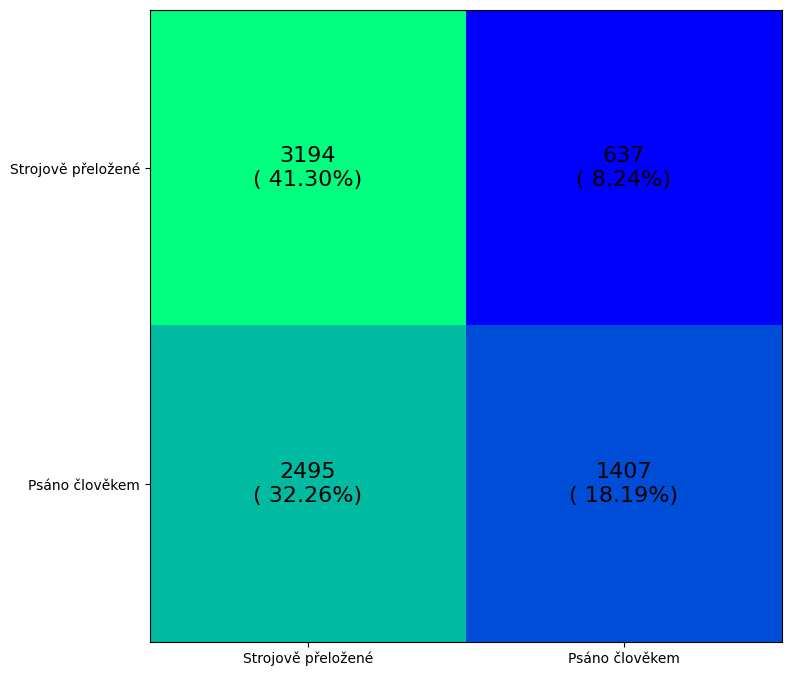
\includegraphics[width=0.6\textwidth]{Figures/MULTI_GRU_GLOVE_conf.png}
	\caption{Výsledné predikování GRU s technikou GloVe modelu na testovacích datech zobrazené v confusion matrix}\label{fig:MULTI GRU GloVe model conf}
\end{figure}

Graf confusion matice~\ref{fig:MULTI GRU Attention model conf} pro klasifikátor GRU s technikou Attention.
\begin{figure}[H]
	\centering
	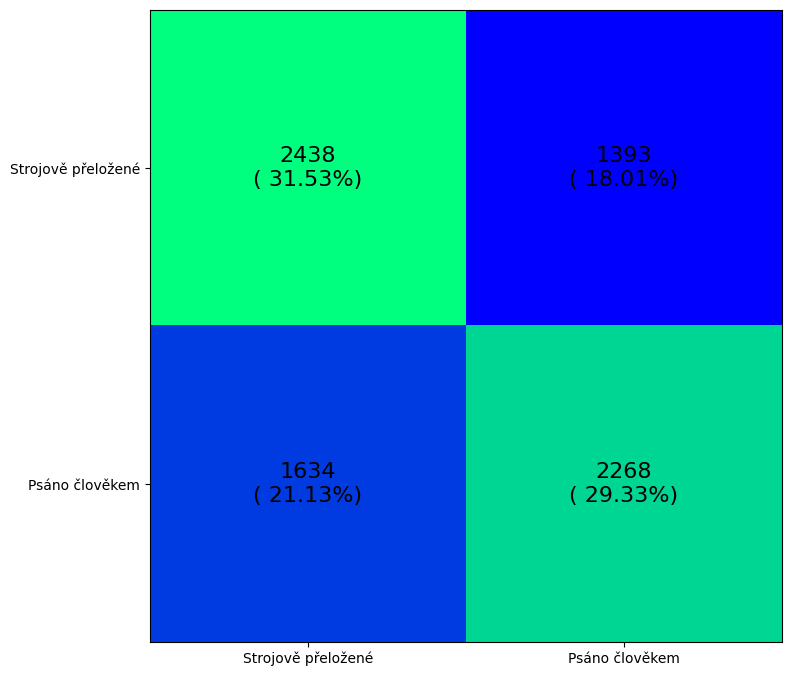
\includegraphics[width=0.6\textwidth]{Figures/MULTI_GRU_Attention_conf.png}
	\caption{Výsledné predikování GRU s technikou Attention modelu na testovacích datech zobrazené v confusion matrix}\label{fig:MULTI GRU Attention model conf}
\end{figure}

Graf confusion matice~\ref{fig:MULTI BERT model conf} pro klasifikátor BERT.\@
\begin{figure}[H]
	\centering
	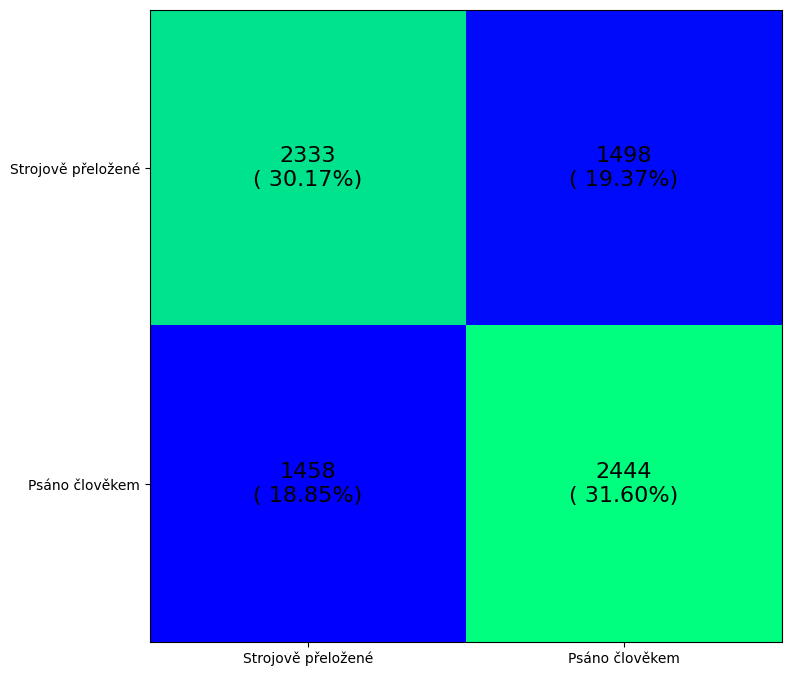
\includegraphics[width=0.6\textwidth]{Figures/MULTI_BERT_conf.png}
	\caption{Výsledné predikování BERT modelu na testovacích datech zobrazené v confusion matrix}\label{fig:MULTI BERT model conf}
\end{figure}

Většina klasifikátorů předpovídá vyváženě jak pro detekci strojově přeložených, tak i člověkem psaných vět.
Nicméně klasifikátor GRU s technikou GloVe se od ostatních klasifikátorů liší a vykazuje větší tendenci k predikci vět psaných člověkem.


\subsubsection{Predikce na reálných datech}
Pro reálná data byla vybrána věta `I am a very smart robot writting the message'.
V následující tabulce~\ref{tab:MULTI predikce} jsou uvedeny predikce jednotlivých klasifikátorů.
Jelikož tato věta byla psána autorem práce, správnou predikcí je `psáno člověkem'.

\begin{table}[H]
	\centering
	\caption{Predikce na reálné větě}\label{tab:MULTI predikce}
	\begin{tabular}{ c c c }
			\toprule
			Klasifikátor & predikční skóre & interpretace skóre\\
			\midrule
			\textbf{LSTM} & \textbf{0.59068} & \textbf{Psáno člověkem}\\
			\textbf{LSTM s technikou GloVe} & \textbf{0.96997} & \textbf{Psáno člověkem}\\
			\textbf{LSTM s technikou Attention} & \textbf{0.97166} & \textbf{Psáno člověkem}\\
			\textbf{GRU} & \textbf{0.54896} & \textbf{Psáno člověkem}\\
			GRU s technikou GloVe & 0.42217 & Strojově přeloženo\\
			\textbf{GRU s technikou Attention} & \textbf{0.81786} & \textbf{Psáno člověkem}\\
			\textbf{BERT} & \textbf{0.85771} & \textbf{Psáno člověkem}\\
			\midrule
		\end{tabular}
\end{table}

Všechny klasifikátory s výjimkou GRU s technikou GloVe byly schopné správně předpovědět odpověď.

\section{Porovnání klasifikátorů}
Pro porovnání klasifikátorů budou použity tři kritéria, na jejichž základě se budou hodnotit klasifikátory.
Tato kritéria jsou:

\begin{itemize}\label{Kritéria}
	\item Počet parametrů: Bude se měřit, kolik parametrů má každý klasifikátor. Tento ukazatel nám poskytne představu o složitosti a velikosti jednotlivých modelů.
	\item Doba trénování: Bude se sledovat, jak dlouho trvá trénování každého klasifikátoru. Toto kritérium nám umožní porovnat rychlost trénování a zjistit, který model se trénuje nejrychleji.
	\item Metrika přesnosti na testovacích datech: Bude se vyhodnocovat přesnost každého klasifikátoru na testovacích datech. Tím získáme informaci o schopnosti jednotlivých modelů správně klasifikovat neznámá data.
\end{itemize}

Na základě těchto tří kritérií budeme schopni porovnat a vyhodnotit jednotlivé klasifikátory.

\subsection{Porovnání počtu parametrů}
Obecně platí, že čím větší počet parametrů má model, tím větší je jeho kapacita a tím lépe by měl být schopen se naučit složitější úlohy.
Parametry modelu představují váhy a biasy, které se optimalizují během trénování, aby model co nejlépe popsal vztahy mezi vstupy a výstupy.

Model s vyšším počtem parametrů má větší flexibilitu při aproximaci složitých funkcí a může se přizpůsobit složitějším vzorům ve vstupních datech.
Avšak vyšší počet parametrů může také způsobit přetrénování, kdy se model naučí příliš specifickým detailům trénovacích dat a nemusí se dobře generalizovat na nová neznámá data.

Optimální počet parametrů závisí na konkrétní úloze a dostupných datových sadách.
V některých případech mohou menší modely s nižším počtem parametrů dosahovat podobných výsledků jako velké modely, pokud je trénování provedeno správně a jsou použity vhodné metody regularizace.

Je důležité najít vyváženou rovnováhu mezi počtem parametrů a schopností modelu se naučit a generalizovat úlohu.

\subsubsection{Porovnání počtu parametrů na anglickém datasetu}
Průměrný počet parametrů klasifikátorů~\ref{tab:res pocet parametru} se pohybuje kolem 2.7 milionů parametrů.
Existuje však výjimka v podobě klasifikátoru BERT, který má přibližně 28 milionů parametrů.
Tento rozdíl je způsoben složitostí a velikostí samotného modelu BERT.\@

\begin{table}[H]
	\centering
	\caption{Počty parametrů klasifikátorů}\label{tab:res pocet parametru}
	\begin{tabular}{ c c }
			\toprule
			Klasifikátor & počet parametrů\\
			\midrule
			LSTM & 3 179 905\\
			GRU & 2 984 321\\         
			LSTM s technikou GloVe & 2 604 009\\         
			GRU s technikou GloVe & 2 422 761\\         
			LSTM s technikou Attention & 3 180 417\\         
			GRU s technikou Attention & 2 984 833\\         
			\textbf{BERT} & \textbf{28 764 162}\\         
			\midrule
		\end{tabular}
\end{table}

\subsubsection{Porovnání počtu parametrů na více jazyčném datasetu}
Většina klasifikátorů~\ref{tab:MULTI res pocet parametru} má přibližně 5,7 milionů parametrů.
Klasifikátory používající techniku GloVe mají přibližně 8,7 milionů parametrů.
Klasifikátor BERT, s přibližně 28 miliony parametrů, má největší počet parametrů mezi všemi zkoumanými klasifikátory.

\begin{table}[H]
	\centering
	\caption{Počty parametrů klasifikátorů}\label{tab:MULTI res pocet parametru}
	\begin{tabular}{ c c }
			\toprule
			Klasifikátor & počet parametrů\\
			\midrule
			LSTM & 5 861 761\\
			GRU & 5 698 945\\         
			LSTM s technikou GloVe & 8 815 889\\         
			GRU s technikou GloVe & 8 634 641\\         
			LSTM s technikou Attention & 5 862 273\\         
			GRU s technikou Attention & 5 699 457\\      
			\textbf{BERT} & \textbf{28 764 162}\\         
			\midrule
		\end{tabular}
\end{table}

\subsection{Porovnání doby trénování}
Doba trénování modelu závisí na jeho komplexnosti, dostupných výpočetních prostředcích a zvolené konfiguraci trénování.
Je důležité správně nastavit parametry trénování, jako je velikost dávky (batch size), rychlost učení (learning rate), počet epoch a další hyperparametry, aby se dosáhlo optimálního výkonu modelu.

Není pravidlem, že co nejdéle trvající trénování vede k nejlepším výsledkům.
Je zapotřebí správně naladit model a jeho hyperparametry a vyhnout se přetrénování (overfittingu) nebo podtrénování (underfittingu).
To znamená, že model by měl být dostatečně komplexní, aby se naučil relevantní vzory ve vstupních datech, ale zároveň by měl být schopný generalizovat na nová data.

\subsubsection{Klasifikátory trénovány na anglickém datasetu}\label{subsec:EN cas}
Doba trénování různých klasifikátorů~\ref{tab:res doba trenovani} tvoří podobné dvojice, kde techniky mají blízkou dobu trénování.
Například v případě GloVe je rozdíl v době trénování mezi architekturami LSTM a GRU pouhých 17 vteřin.

Podobnost mezi těmito dvojicemi je způsobena nastavením počtu epoch pro trénování klasifikátorů.
Když jsou stejné techniky natrénovány s podobným nebo identickým počtem epoch na trénovacích datech, dochází ke vzniku těchto podobností v době trénování.

Učení BERTa trvá nejdelší dobu z důvodu jeho složitosti a rozsáhlých parametrů~\ref{tab:res pocet parametru}.
BERT se stal jedním z nejvýkonnějších modelů pro zpracování přirozeného jazyka, ale jeho trénování vyžaduje více času kvůli jeho komplexní struktuře a většímu počtu parametrů.

\begin{table}[H]
	\centering
	\caption{Celková doba trénování klasifikátorů}\label{tab:res doba trenovani}
	\begin{tabular}{ c c }
			\toprule
			Klasifikátor & doba trénování\\
			\midrule
			LSTM & 541s\\
			GRU & 566s\\         
			LSTM s technikou GloVe & 661s\\         
			GRU s technikou GloVe & 644s\\         
			LSTM s technikou Attention & 426s\\         
			GRU s technikou Attention & 396s\\         
			\textbf{BERT} & \textbf{1024s}\\         
			\midrule
		\end{tabular}
\end{table}

\subsubsection{Klasifikátory trénovány na více jazyčném datasetu}
Doba trénování různých klasifikátorů~\ref{tab:MULTI res doba trenovani} tvoří podobné dvojice, ze stejných důvodů jako pro anglický dataset viz.~\ref{subsec:EN cas}.

Rozdíl v době trénování mezi klasifikátory anglického datasetu a klasifikátory tohoto datasetu je způsoben větším rozsahem více jazyčného datasetu, na kterém museli být klasifikátory natrénovány.
Větší datasety vyžadují delší dobu pro kompletní naučení modelu, jelikož je nutné zpracovat a analyzovat větší množství datových instancí.
To může zpomalit celkový proces trénování a prodloužit dobu potřebnou k dosažení požadované úrovně výkonu klasifikátoru.
Je důležité brát v úvahu velikost datasetu a jeho vliv na dobu trénování při srovnávání klasifikátorů.

Učení BERTa trvá nejdelší dobu z důvodu jeho složitosti a rozsáhlých parametrů~\ref{tab:MULTI res pocet parametru}.

\begin{table}[H]
	\centering
	\caption{Celková doba trénování klasifikátorů}\label{tab:MULTI res doba trenovani}
	\begin{tabular}{ c c }
			\toprule
			Klasifikátor & doba trénování\\
			\midrule
			LSTM & 851s\\
			GRU & 816s\\         
			LSTM s technikou GloVe & 907s\\         
			GRU s technikou GloVe  & 937s\\         
			LSTM s technikou Attention & 781s\\         
			GRU s technikou Attention & 780s\\         
			\textbf{BERT} & \textbf{9049s}\\         
			\midrule
		\end{tabular}
\end{table}


\subsection{Porovnání v rámci metriky přesnosti nad testovacími daty}
Metrika přesnosti je jednou z nejčastěji používaných metrik pro vyhodnocování přesnosti klasifikátorů.
Metrika přesnosti udává, jaký podíl správně klasifikovaných instancí má model ze všech klasifikovaných instancí.

V případě porovnání klasifikátorů pro detekci strojově přeložených a ručně psaných sekvencí textu, metrika přesnosti nám poskytne informaci o tom, jak dobře tyto klasifikátory rozlišují mezi těmito dvěma typy sekvencí.
Vyšší přesnost znamená, že model správně identifikuje většinu strojově přeložených a ručně psaných sekvencí.

\subsubsection{Klasifikátory trénovány na anglickém datasetu}
Finální a nejdůležitější porovnání mezi klasifikátory je na základě metriky přesnosti~\ref{tab:res metrika presnosti}.
Všechny modely dosáhly přesnosti vyšší než 60 \%, přičemž nejvyšší přesnost zaznamenal klasifikátor BERT s hodnotou 66 \%.

Tento výsledek naznačuje, že BERT je nejefektivnějším klasifikátorem v daném kontextu.
Je však také důležité vzít v úvahu další faktory, jako jsou rychlost trénování, náročnost implementace a případné omezení modelu v praxi.
Nicméně z hlediska dosažené přesnosti se klasifikátor BERT ukazuje jako nejlepší volba mezi zkoumanými modely.

\begin{table}[H]
	\centering
	\caption{Metrika přesnosti klasifikátorů}\label{tab:res metrika presnosti}
	\begin{tabular}{ c c }
			\toprule
			Klasifikátor & přesnost\\
			\midrule
			LSTM & 63 \%\\
			GRU & 60 \%\\         
			LSTM s technikou GloVe & 61 \%\\         
			GRU s technikou GloVe & 65 \%\\         
			LSTM s technikou Attention & 63 \%\\         
			GRU s technikou Attention & 64 \%\\         
			\textbf{BERT} & \textbf{66 \%} \\         
			\midrule
		\end{tabular}
\end{table}

\subsubsection{Klasifikátory trénovány na více jazyčném datasetu}
Finální a nejdůležitější porovnání mezi klasifikátory se provádí na základě metriky přesnosti~\ref{tab:MULTI res metrika presnosti}.
Všechny modely dosáhly přesnosti, která je buď stejná nebo vyšší než 60 \%.
Nejvyšší přesnost byla dosažena klasifikátorem BERT a klasifikátorem GRU s technikou attention, které oba dosáhly přesnosti 63 \%.

Na základě informací o velikosti modelu~\ref{tab:MULTI res pocet parametru}, době trénování~\ref{tab:MULTI res doba trenovani} a dosažené metrice přesnosti~\ref{tab:MULTI res metrika presnosti} lze usoudit, že nejlepším klasifikátorem je architektura GRU s použitím attention techniky, i přestože klasifikátor BERT dosáhl stejné přesnosti.
Tento závěr je podpořen faktem, že klasifikátor BERT vyžadoval mnohem delší dobu trénování než GRU s technikou attention.
Tedy GRU s attention technikou je schopný dosáhnout stejné přesnosti jako BERT v kratším čase, jelikož je méně komplexní, což jej činí efektivnějším z hlediska časového a výpočetního.
\begin{table}[H]
	\centering
	\caption{Metrika přesnosti klasifikátorů}\label{tab:MULTI res metrika presnosti}
	\begin{tabular}{ c c }
			\toprule
			Klasifikátor & přesnost\\
			\midrule
			LSTM & 61 \%\\
			GRU & 61 \%\\         
			LSTM s technikou GloVe & 61 \%\\         
			GRU s technikou GloVe & 60 \%\\         
			LSTM s technikou Attention & 60 \%\\         
			\textbf{GRU s technikou Attention} & \textbf{63 \%}\\         
			\textbf{BERT} & \textbf{63 \%} \\         
			\midrule
		\end{tabular}
\end{table}

% \section{Vyhodnocení nad Anglickým datovým souborem}

% \subsection{LSTM model}\label{ref:LSTM model}
% Architektura tohoto modelu je postavena na vylepšené verzi RNN zvané Long-Short term memory\@.

% Samotná architektura modelu je sepsána v tabulce~\ref{tab:LSTM model}.
% \begin{table}[H]
% 	\centering
% 	\caption{LSTM model}\label{tab:LSTM model}
% 	\begin{tabular}{ c c c }
% 			\toprule
% 			Vrstva modelu & výstupný formát dat & počet parametrů\\
% 			\midrule
%             TextVectorization & (None, 256) & 0\\         
%             Embedding & (None, 256, 256) & 1489664\\   
%             Bidirectional & (None, 256, 256) & 394240\\    
%             Bidirectional & (None, 256) & 394240\\  
%             Dense & (None, 256) & 65792\\  
%             Dropout & (None, 256) & 0\\   
%             Dense & (None, 1) & 257\\ 
% 			\midrule
% 		\end{tabular}
% \end{table}
% Z této tabulky vyplývá její rozložení do vrstev.
% Nejdříve je vrstva, která zpracovává text jako takový a odstraňuje z něj přebytečné bílé znaky atd..
% Následuje vrstva s embedding technikou, která převádí tokeny do vektorové podoby.
% Zde je již logická stránka modelu a to dvě po sobě jdoucí bidirectional LSTM vrstvy se 128 neurony, které se doplňují informaci.
% Plně propojená vrstva s 256ti neurony je zapojena hned po bidirectional vrstvách.
% Zakončuje to jednoduchý Dropout a plně propojená vrstva s jedním rozhodovacím neuronem, který určuje zdali text byl přeložen strojově či nikoli.

% Pro zajímavost počet trénovacích a netrénovacích parametrů~\ref{src:LSTM model parametry}.
% \begin{lstlisting}[label=src:LSTM model parametry,caption={LSTM model parametry}]
%     Total params: 2,344,193
%     Trainable params: 2,344,193
%     Non-trainable params: 0 
% \end{lstlisting}

% Výsledek naučeného modelu~\ref{src:LSTM model trenovani}.
% \begin{lstlisting}[label=src:LSTM model trenovani,caption={LSTM model trenování}]
%     LSTM Loss:  1.317
%     LSTM Accuracy:  0.647
% \end{lstlisting}

% Tento model se naučil na 50ti epochách za tento čas~\ref{src:LSTM model casy}.
% \begin{lstlisting}[label=src:LSTM model casy,caption={LSTM model časy}]
%     Training time [LSTM]: 81s
% \end{lstlisting}

% Historie učení~\ref{fig:LSTM model trenovani}.
% \begin{figure}[H]
% 	\centering
% 	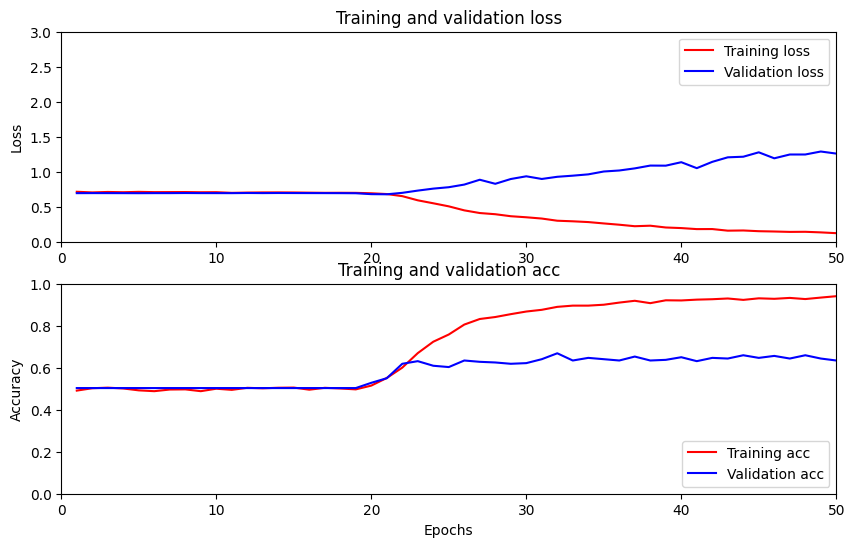
\includegraphics[width=0.7\textwidth]{Figures/LSTM_train.png}
% 	\caption{LSTM model průběhu trénování}\label{fig:LSTM model trenovani}
% \end{figure}

% \begin{table}[H]
% 	\centering
% 	\caption{LSTM model hodnoty trénování}\label{tab:LSTM model hodnoty trenovani}
% 	\begin{tabular}{ c c c c c c c }
% 			\toprule
% 			Epocha & 1. & 10. & 20. & 30. & 40. & 50. \\
% 			\midrule
% 			Přesnost & 49\% & 50\% & 51\% & 86\% & 92\% & 94\% \\
% 			Val. Přesnost & 50\% & 50\% & 52\% & 62\% & 65\% & 63\% \\
% 			Loss & 0.71 & 0.71 & 0.69 & 0.35 & 0.19 & 0.12 \\
% 			Val. Loss & 0.69 & 0.69 & 0.68 & 0.93 & 1.14 & 1.26 \\
% 			\midrule
% 		\end{tabular}
% \end{table}

% Confusion matice, pro lepší porozumění předpovídajícího modelu~\ref{fig:LSTM model confusion matice}.
% \begin{figure}[H]
% 	\centering
% 	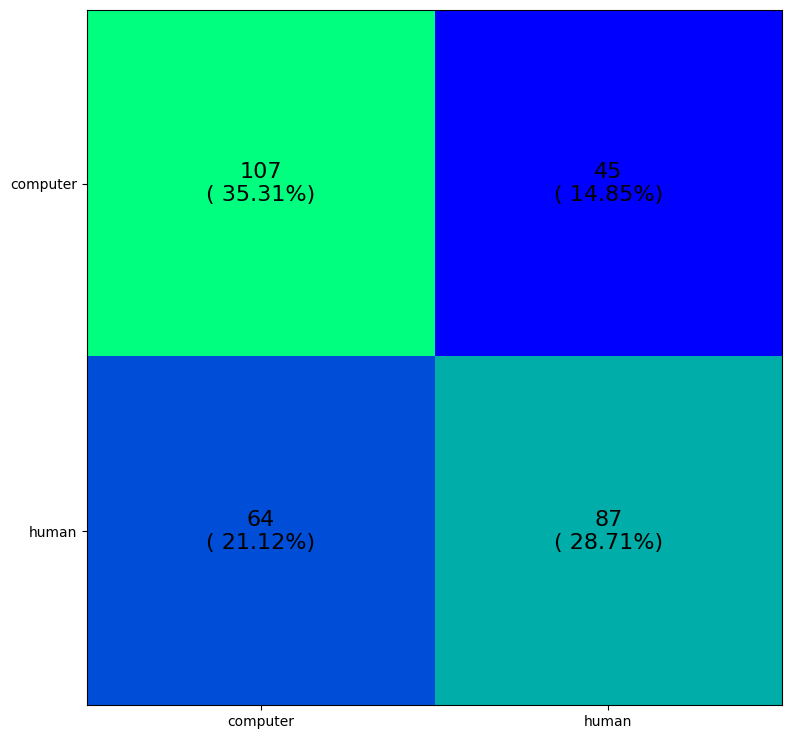
\includegraphics[width=0.6\textwidth]{Figures/LSTM_conf.png}
% 	\caption{LSTM model confusion matice}\label{fig:LSTM model confusion matice}
% \end{figure}

% \subsubsection{Výsledek modelu}
% Podle grafu učení lze vidět, že daný model byl schopen se naučit skvěle na trénovacích datech.
% Bohužel na testovacích datech model už nedopadl.

% Podle confusion matice model dokáže rozeznávat texty psané člověkem nebo počítačem docela rovnoměrně. Není zde jednostranná predikce.


% \subsection{GRU model}\label{ref:GRU model}
% Architektura tohoto modelu je postavena na vylepšené verzi RNN zvané Gated Recurrent Unit\@.

% Architektura modelu je sepsána v tabulce~\ref{tab:GRU model}.
% \begin{table}[H]
% 	\centering
% 	\caption{GRU model}\label{tab:GRU model}
% 	\begin{tabular}{ c c c }
% 			\toprule
% 			Vrstva modelu & výstupný formát dat & počet parametrů\\
% 			\midrule
%             TextVectorization & (None, 256) & 0\\         
%             Embedding & (None, 256, 256) & 1489664\\   
%             Bidirectional & (None, 256, 256) & 296448\\    
%             Bidirectional & (None, 256) & 296448\\  
%             Dense & (None, 256) & 65792\\  
%             Dropout & (None, 256) & 0\\   
%             Dense & (None, 1) & 257\\ 
% 			\midrule
% 		\end{tabular}
% \end{table}
% Z této tabulky vyplývá její rozložení do vrstev.
% Nejdříve je vrstva, která zpracovává text jako takový a odstraňuje z něj přebytečné bílé znaky atd..
% Následuje vrstva embedding technika, která převádí tokeny do vektorové podoby.
% Zde je již logická stránka modelu a to dvě po sobě jdoucí bidirectional GRU vrstvy se 128 neurony, které se doplňují informaci.
% Plně propojená vrstva s 256ti neurony je zapojena hned po bidirectional vrstvách.
% Zakončuje to jednoduchý Dropout a plně propojená vrstva s jedním rozhodovacím neuronem, který určuje zdali text byl přeložen strojově či nikoli.

% Pro zajímavost počet trénovacích a netrénovacích parametrů~\ref{src:GRU model parametry}.
% \begin{lstlisting}[label=src:GRU model parametry,caption={GRU model parametry}]
%     Total params: 2,148,609
%     Trainable params: 2,148,609
%     Non-trainable params: 0 
% \end{lstlisting}

% Výsledek naučeného modelu~\ref{src:GRU model trenovani}.
% \begin{lstlisting}[label=src:GRU model trenovani,caption={GRU model trenování}]
%     GRU Loss:  1.596
%     GRU Accuracy:  0.617
% \end{lstlisting}

% Tento model se naučil na 50ti epochách za tento čas~\ref{src:GRU model casy}.
% \begin{lstlisting}[label=src:GRU model casy,caption={GRU model časy}]
%     Training time [GRU]: 76s
% \end{lstlisting}

% Historie učení~\ref{fig:GRU model trenovani}.
% \begin{figure}[H]
% 	\centering
% 	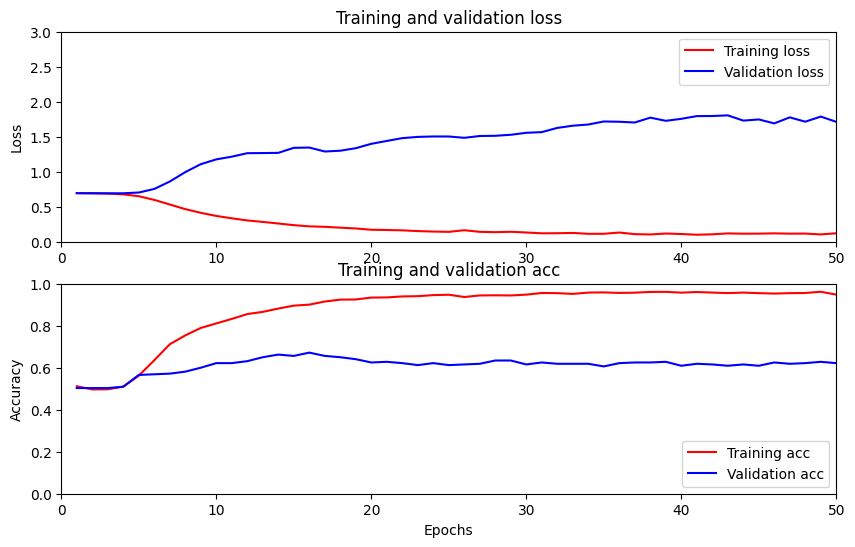
\includegraphics[width=0.7\textwidth]{Figures/GRU_train.png}
% 	\caption{GRU model průběhu trénování}\label{fig:GRU model trenovani}
% \end{figure}

% \begin{table}[H]
% 	\centering
% 	\caption{GRU model hodnoty trénování}\label{tab:GRU model hodnoty trenovani}
% 	\begin{tabular}{ c c c c c c c }
% 			\toprule
% 			Epocha & 1. & 10. & 20. & 30. & 40. & 50. \\
% 			\midrule
% 			Přesnost & 51\% & 81\% & 93\% & 94\% & 95\% & 94\% \\
% 			Val. Přesnost & 50\% & 62\% & 62\% & 61\% & 60\% & 62\% \\
% 			Loss & 0.69 & 0.37 & 0.17 & 0.13 & 0.11 & 0.12 \\
% 			Val. Loss & 0.69 & 1.18 & 1.40 & 1.56 & 1.76 & 1.71 \\
% 			\midrule
% 		\end{tabular}
% \end{table}

% Confusion matice, pro lepší porozumění předpovídajícího modelu~\ref{fig:GRU model confusion matice}.
% \begin{figure}[H]
% 	\centering
% 	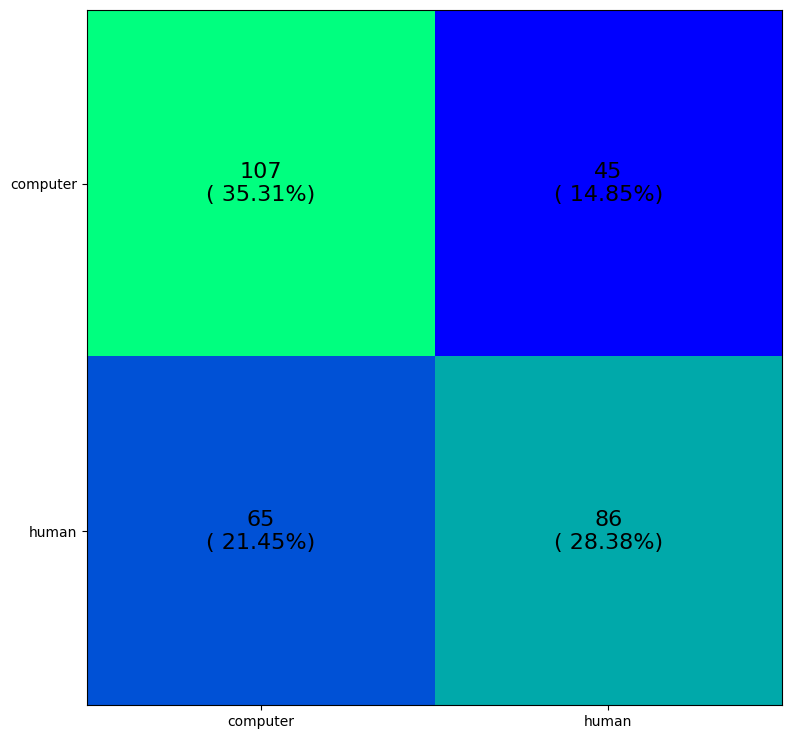
\includegraphics[width=0.6\textwidth]{Figures/GRU_conf.png}
% 	\caption{GRU model confusion matice}\label{fig:GRU model confusion matice}
% \end{figure}

% \subsubsection{Výsledek modelu}
% Tato architektura modelu měla podobné výsledky po vzoru LSTM modelu.
% Podle grafu učení lze vidět, že daný model byl schopen se naučit skvěle na trénovacích datech.
% Bohužel na testovacích datech model už nedopadl.

% Podle confusion matice model více predikuje texty na stranu strojově přeložených.


% \subsection{GloVe + LSTM model}\label{ref:GloVe LSTM model}
% Architektura tohoto modelu je víceméně stejná jako pro LSTM model, pouze v tomto modelu se převzala embedding technika GloVe.

% GloVe má v nabídce několik před trénovaných modelů s embedding technikou.
% V této práci se používá model, který je před trénován nad šesti miliardami tokenů, ze kterých vznikl slovník s 400 tisíci unikátních slov.
% A každé slovo je popsáno 200 dimenzionálním vektorem.

% Architektura modelu je sepsána v tabulce~\ref{tab:LSTM model}.

% Jiná embedding technika, zapříčiní změnu v počtu parametrů~\ref{src:GloVe LSTM model parametry}.
% \begin{lstlisting}[label=src:GloVe LSTM model parametry,caption={GloVe LSTM model parametry}]
%     Total params: 1,961,385
%     Trainable params: 797,185
%     Non-trainable params: 1,164,200
% \end{lstlisting}

% Výsledek naučeného modelu~\ref{src:GloVe LSTM model trenovani}.
% \begin{lstlisting}[label=src:GloVe LSTM model trenovani,caption={GloVe LSTM model trenování}]
%     GLOVE_LSTM Loss:  1.782
%     GLOVE_LSTM Accuracy:  0.564
% \end{lstlisting}

% Tento model se naučil na 50ti epochách za tento čas~\ref{src:GloVe LSTM model casy}.
% \begin{lstlisting}[label=src:GloVe LSTM model casy,caption={GloVe LSTM model časy}]
%     Training time [GLOVE_LSTM]: 76s
% \end{lstlisting}

% Historie učení~\ref{fig:GloVe LSTM model trenovani}.
% \begin{figure}[H]
% 	\centering
% 	\includegraphics[width=0.7\textwidth]{Figures/glove_LSTM_train.png}
% 	\caption{GloVe LSTM model průběhu trénování}\label{fig:GloVe LSTM model trenovani}
% \end{figure}

% \begin{table}[H]
% 	\centering
% 	\caption{GloVe LSTM model hodnoty trénování}\label{tab:GloVe LSTM model hodnoty trenovani}
% 	\begin{tabular}{ c c c c c c c }
% 			\toprule
% 			Epocha & 1. & 10. & 20. & 30. & 40. & 50. \\
% 			\midrule
% 			Přesnost & 51\% & 51\% & 67\% & 87\% & 92\% & 91\% \\
% 			Val. Přesnost & 50\% & 50\% & 54\% & 58\% & 59\% & 60\% \\
% 			Loss & 0.72 & 0.70 & 0.57 & 0.29 & 0.18 & 0.19 \\
% 			Val. Loss & 0.69 & 0.69 & 0.86 & 1.31 & 1.51 & 1.59 \\
% 			\midrule
% 		\end{tabular}
% \end{table}

% Confusion matice, pro lepší porozumění předpovídajícího modelu~\ref{fig:GloVe LSTM model confusion matice}.
% \begin{figure}[H]
% 	\centering
% 	\includegraphics[width=0.6\textwidth]{Figures/glove_lstm_conf.png}
% 	\caption{GloVe LSTM model confusion matice}\label{fig:GloVe LSTM model confusion matice}
% \end{figure}

% \subsubsection{Výsledek modelu}
% Tato architektura modelu měla být o něco lepší než byla architektura LSTM postavená na vlastní embedding technice, to se ale na testovacích datech neprokázalo.

% Podle grafu učení lze vidět, že daný model byl schopen se naučit skvěle na trénovacích datech.
% Bohužel na testovacích datech model už nedopadl.

% Podle confusion matice model dokáže rozeznávat texty psané člověkem nebo počítačem docela rovnoměrně. Není zde jednostranná predikce.


% \subsection{GloVe + GRU model}\label{ref:GLOVE GRU model}
% Architektura tohoto modelu je víceméně stejná jako pro GRU model, pouze v tomto modelu se převzala embedding technika GloVe.

% GloVe má v nabídce několik před trénovaných modelů s embedding technikou.
% V této práci se používá model, který je před trénován nad šesti miliardami tokenů, ze kterých vznikl slovník s 400 tisíci unikátních slov.
% A každé slovo je popsáno 200 dimenzionálním vektorem.

% Architektura modelu je sepsána v tabulce~\ref{tab:GRU model}.

% Jiná embedding technika, zapříčiní změnu v počtu parametrů~\ref{src:GloVe GRU model parametry}.
% \begin{lstlisting}[label=src:GloVe GRU model parametry,caption={GloVe GRU model parametry}]
%     Total params: 1,780,137
%     Trainable params: 615,937
%     Non-trainable params: 1,164,200
% \end{lstlisting}

% Výsledek naučeného modelu~\ref{src:GloVe GRU model trenovani}.
% \begin{lstlisting}[label=src:GloVe GRU model trenovani,caption={GloVe GRU model trenování}]
%     GloVe_GRU Loss:  2.032
%     GloVe_GRU Accuracy:  0.624
% \end{lstlisting}

% Tento model se naučil na 50ti epochách za tento čas~\ref{src:GloVe GRU model casy}.
% \begin{lstlisting}[label=src:GloVe GRU model casy,caption={GloVe GRU model časy}]
%     Training time [GloVe_GRU]: 74s
% \end{lstlisting}

% Historie učení~\ref{fig:GloVe GRU model trenovani}.
% \begin{figure}[H]
% 	\centering
% 	\includegraphics[width=0.7\textwidth]{Figures/glove_gru_train.png}
% 	\caption{GloVe GRU model průběhu trénování}\label{fig:GloVe GRU model trenovani}
% \end{figure}

% \begin{table}[H]
% 	\centering
% 	\caption{GloVe GRU model hodnoty trénování}\label{tab:GloVe GRU model hodnoty trenovani}
% 	\begin{tabular}{ c c c c c c c }
% 			\toprule
% 			Epocha & 1. & 10. & 20. & 30. & 40. & 50. \\
% 			\midrule
% 			Přesnost & 51\% & 56\% & 70\% & 86\% & 91\% & 93\% \\
% 			Val. Přesnost & 50\% & 52\% & 54\% & 62\% & 60\% & 60\% \\
% 			Loss & 0.72 & 0.67 & 0.54 & 0.28 & 0.19 & 0.14 \\
% 			Val. Loss & 0.69 & 0.70 & 0.85 & 1.32 & 1.77 & 1.78 \\
% 			\midrule
% 		\end{tabular}
% \end{table}

% Confusion matice, pro lepší porozumění předpovídajícího modelu~\ref{fig:GloVe GRU model confusion matice}.
% \begin{figure}[H]
% 	\centering
% 	\includegraphics[width=0.6\textwidth]{Figures/glove_gru_conf.png}
% 	\caption{GloVe GRU model confusion matice}\label{fig:GloVe GRU model confusion matice}
% \end{figure}

% \subsubsection{Výsledek modelu}
% Tato architektura modelu měla být o něco lepší než byla architektura GRU postavená na vlastní embedding technice, to se ale na testovacích datech neprokázalo.

% Podle grafu učení lze vidět, že daný model byl schopen se naučit skvěle na trénovacích datech.
% Bohužel na testovacích datech model už nedopadl.

% Podle confusion matice model více predikuje texty na stranu strojově přeložených.


% \subsection{Attention + LSTM model}\label{ref:Attention LSTM model}
% Architektura tohoto modelu je víceméně stejná jako pro LSTM model, pouze v tomto modelu se přidala tzv.~Attention vrstva, která by měla model podstatně vylepšit.
% Architektura modelu je sepsána v tabulce~\ref{tab:Attention LSTM model}.

% \begin{table}[H]
% 	\centering
% 	\caption{Attention LSTM model}\label{tab:Attention LSTM model}
% 	\begin{tabular}{ c c c }
% 			\toprule
% 			Vrstva modelu & výstupný formát dat & počet parametrů\\
% 			\midrule
%             TextVectorization & (None, 256) & 0\\         
%             Embedding & (None, 256, 256) & 1489664\\   
%             Bidirectional & (None, 256, 256) & 394240\\    
%             Bidirectional & (None, 256) & 394240\\  
%             Attention & (None, 256) & 512\\
%             Dense & (None, 256) & 65792\\  
%             Dropout & (None, 256) & 0\\   
%             Dense & (None, 1) & 257\\ 
% 			\midrule
% 		\end{tabular}
% \end{table}
% Z této tabulky vyplývá její rozložení do vrstev.
% Nejdříve je vrstva, která zpracovává text jako takový a odstraňuje z něj přebytečné bílé znaky atd..
% Následuje vrstva s embedding technikou, která převádí tokeny do vektorové podoby.
% Zde je již logická stránka modelu a to dvě po sobě jdoucí bidirectional LSTM vrstvy se 128 neurony, které se doplňují informaci.
% Tady, na rozdíl od původního LSTM modelu, přibyla Attention vrstva, která přepočítává vektory.
% Plně propojená vrstva s 256ti neurony je zapojena hned po Attention vrstvě.
% Zakončuje to jednoduchý Dropout a plně propojená vrstva s jedním rozhodovacím neuronem, který určuje zdali text byl přeložen strojově či nikoli.


% Pro zajímavost počet trénovacích a netrénovacích parametrů~\ref{src:Attention LSTM model parametry}.
% Kvůli přidané vrstvě ani počet parametrů není stejným oproti modelu LSTM\@.
% \begin{lstlisting}[label=src:Attention LSTM model parametry,caption={Attention LSTM model parametry}]
%     Total params: 2,344,705
%     Trainable params: 2,344,705
%     Non-trainable params: 0
% \end{lstlisting}

% Výsledek naučeného modelu~\ref{src:Attention LSTM model trenovani}.
% \begin{lstlisting}[label=src:Attention LSTM model trenovani,caption={Attention LSTM model trenování}]
%     Attention_LSTM Loss:  1.961
%     Attention_LSTM Accuracy:  0.667
% \end{lstlisting}

% Tento model se naučil na 50ti epochách za tento čas~\ref{src:Attention LSTM model casy}.
% \begin{lstlisting}[label=src:Attention LSTM model casy,caption={Attention LSTM model časy}]
%     Training time [Attention_LSTM]: 86s
% \end{lstlisting}

% Historie učení~\ref{fig:Attention LSTM model trenovani}.
% \begin{figure}[H]
% 	\centering
% 	\includegraphics[width=0.7\textwidth]{Figures/Attention_LSTM_train.png}
% 	\caption{Attention LSTM model průběhu trénování}\label{fig:Attention LSTM model trenovani}
% \end{figure}

% \begin{table}[H]
% 	\centering
% 	\caption{Attention LSTM model hodnoty trénování}\label{tab:Attention LSTM model hodnoty trenovani}
% 	\begin{tabular}{ c c c c c c c }
% 			\toprule
% 			Epocha & 1. & 10. & 20. & 30. & 40. & 50. \\
% 			\midrule
% 			Přesnost & 50\% & 86\% & 91\% & 92\% & 92\% & 92\% \\
% 			Val. Přesnost & 50\% & 61\% & 65\% & 65\% & 65\% & 64\% \\
% 			Loss & 0.76 & 0.28 & 0.13 & 0.10 & 0.11 & 0.10 \\
% 			Val. Loss & 0.70 & 1.16 & 1.93 & 2.10 & 2.13 & 2.25 \\
% 			\midrule
% 		\end{tabular}
% \end{table}

% Confusion matice, pro lepší porozumění předpovídajícího modelu~\ref{fig:Attention LSTM model confusion matice}.
% \begin{figure}[H]
% 	\centering
% 	\includegraphics[width=0.6\textwidth]{Figures/Attention_LSTM_conf.png}
% 	\caption{Attention LSTM model confusion matice}\label{fig:Attention LSTM model confusion matice}
% \end{figure}

% \subsubsection{Výsledek modelu}
% Tato architektura modelu měla být o něco lepší než byla architektura LSTM\@.
% A na rozdíl od pokusu se GloVe, Attention vrstva skutečně daný model vylepšila.

% Podle grafu učení lze vidět, že daný model byl schopen se naučit skvěle na trénovacích datech.
% Bohužel na testovacích datech model už nedopadl.

% Podle confusion matice je predikce modelu na hraně mezi rovnoměrným predikováním a částečně na stranu strojově přeložených textů.


% \subsection{Attention + GRU model}\label{ref:Attention GRU model}
% Architektura tohoto modelu je víceméně stejná jako pro GRU model, pouze v tomto modelu se přidala tzv.~Attention vrstva, která by měla model podstatně vylepšit.
% Architektura modelu je sepsána v tabulce~\ref{tab:Attention GRU model}.

% \begin{table}[H]
% 	\centering
% 	\caption{Attention GRU model}\label{tab:Attention GRU model}
% 	\begin{tabular}{ c c c }
% 			\toprule
% 			Vrstva modelu & výstupný formát dat & počet parametrů\\
% 			\midrule
%             TextVectorization & (None, 256) & 0\\         
%             Embedding & (None, 256, 256) & 1489664\\   
%             Bidirectional & (None, 256, 256) & 296448\\    
%             Bidirectional & (None, 256) & 296448\\  
%             Attention & (None, 256) & 512\\
%             Dense & (None, 256) & 65792\\  
%             Dropout & (None, 256) & 0\\   
%             Dense & (None, 1) & 257\\ 
% 			\midrule
% 		\end{tabular}
% \end{table}
% Z této tabulky vyplývá její rozložení do vrstev.
% Nejdříve je vrstva, která zpracovává text jako takový a odstraňuje z něj přebytečné bílé znaky atd..
% Následuje vrstva s embedding technikou, která převádí tokeny do vektorové podoby.
% Zde je již logická stránka modelu a to dvě po sobě jdoucí bidirectional GRU vrstvy se 128 neurony, které se doplňují informaci.
% Tady, na rozdíl od původního LSTM modelu, přibyla Attention vrstva, která přepočítává vektory.
% Plně propojená vrstva s 256ti neurony je zapojena hned po Attention vrstvě.
% Zakončuje to jednoduchý Dropout a plně propojená vrstva s jedním rozhodovacím neuronem, který určuje zdali text byl přeložen strojově či nikoli.

% Pro zajímavost počet trénovacích a netrénovacích parametrů~\ref{src:Attention GRU model parametry}.
% Kvůli přidané vrstvě ani počet parametrů není stejným oproti modelu GRU\@.
% \begin{lstlisting}[label=src:Attention GRU model parametry,caption={Attention GRU model parametry}]
%     Total params: 2,149,121
%     Trainable params: 2,149,121
%     Non-trainable params: 0
% \end{lstlisting}

% Výsledek naučeného modelu~\ref{src:Attention GRU model trenovani}.
% \begin{lstlisting}[label=src:Attention GRU model trenovani,caption={Attention GRU model trenování}]
%     Attention_GRU Loss:  1.496
%     Attention_GRU Accuracy:  0.670
% \end{lstlisting}

% Tento model se naučil na 50ti epochách za tento čas~\ref{src:Attention GRU model casy}.
% \begin{lstlisting}[label=src:Attention GRU model casy,caption={Attention GRU model časy}]
%     Training time [Attention_GRU]: 79s
% \end{lstlisting}

% Historie učení~\ref{fig:Attention GRU model trenovani}.
% \begin{figure}[H]
% 	\centering
% 	\includegraphics[width=0.7\textwidth]{Figures/Attention_GRU_train.png}
% 	\caption{Attention GRU model průběhu trénování}\label{fig:Attention GRU model trenovani}
% \end{figure}

% \begin{table}[H]
% 	\centering
% 	\caption{Attention GRU model hodnoty trénování}\label{tab:Attention GRU model hodnoty trenovani}
% 	\begin{tabular}{ c c c c c c c }
% 			\toprule
% 			Epocha & 1. & 10. & 20. & 30. & 40. & 50. \\
% 			\midrule
% 			Přesnost & 50\% & 84\% & 91\% & 92\% & 92\% & 93\% \\
% 			Val. Přesnost & 50\% & 60\% & 61\% & 64\% & 65\% & 64\% \\
% 			Loss & 0.71 & 0.35 & 0.18 & 0.14 & 0.10 & 0.10 \\
% 			Val. Loss & 0.69 & 1.16 & 1.55 & 1.64 & 1.87 & 2.02 \\
% 			\midrule
% 		\end{tabular}
% \end{table}

% Confusion matice, pro lepší porozumění předpovídajícího modelu~\ref{fig:Attention GRU model confusion matice}.
% \begin{figure}[H]
% 	\centering
% 	\includegraphics[width=0.6\textwidth]{Figures/attention_gru_conf.png}
% 	\caption{Attention GRU model confusion matice}\label{fig:Attention GRU model confusion matice}
% \end{figure}

% \subsubsection{Výsledek modelu}
% Tato architektura modelu měla být o něco lepší než byla architektura GRU\@.
% A na rozdíl od pokusu se GloVe, Attention vrstva skutečně daný model vylepšila obdobně jako pomohla u GRU modelu.

% Podle grafu učení lze vidět, že daný model byl schopen se naučit skvěle na trénovacích datech.
% Bohužel na testovacích datech model už nedopadl.

% Podle confusion matice model dokáže rozeznávat texty psané člověkem nebo počítačem docela rovnoměrně. Není zde jednostranná predikce.


% \subsection{BERT model}\label{ref:BERT model}
% Architektura tohoto modelu je oproti ostatním modelům velice odlišná. Podle očekávání by BERT měl dominovat mezi ostatními modely.
% Využívá jak vlastní embedding techniku, attention vrstvy a k tomu i techniku zvanou positional encoding a je postaven na reprezentace enkodéru z Transformer sítě.

% Modelů BERT existuje několik druhů v tomto případě se použije Architektura BERTa se čtyřmi skrytými vrstvami každá čítající 512 neuronů a s osmi attention hlavami.

% Architektura modelu je sepsána v tabulce~\ref{tab:BERT model}.
% \begin{table}[H]
% 	\centering
% 	\caption{BERT model}\label{tab:BERT model}
% 	\begin{tabular}{ c c c }
% 			\toprule
% 			Vrstva modelu & výstupný formát dat & počet parametrů\\
% 			\midrule
%             InputLayer & (None,) & 0\\         
%             Preprocessing & --- & 0\\   
%             BERT encoder & --- & 28,763,649\\    
%             Dropout & (None, 512) & 0\\  
%             Dense & (None, 1) & 513\\ 
% 			\midrule
% 		\end{tabular}
% \end{table}
% Z této tabulky vyplývá její rozložení do vrstev.
% Vrstva přebírající vstup.
% Vrstva zpracovávající vstupní data na data potřebná formátu BERTa.
% Vrstva s modelem BERT\@.
% Vrstva s Dropout technikou, pro zamezení problému over-fitting.
% Vrstva plně propojená síť s jedním neuronem, pro určení binárního rozhodnutí.

% Pro zajímavost počet trénovacích a netrénovacích parametrů~\ref{src:BERT model parametry}.
% BERT obsahuje oproti ostatním modelům o řád vyšší počet parametrů.
% \begin{lstlisting}[label=src:BERT model parametry,caption={BERT model parametry}]
%     Total params: 28,764,162
%     Trainable params: 28,764,161
%     Non-trainable params: 1
% \end{lstlisting}

% Výsledek naučeného modelu~\ref{src:BERT model trenovani}.
% \begin{lstlisting}[label=src:BERT model trenovani,caption={BERT model trenování}]
%     BERT Loss:  0.614
%     BERT Accuracy:  0.611
% \end{lstlisting}

% Tento model se naučil na 50ti epochách za tento čas~\ref{src:BERT model casy}.
% \begin{lstlisting}[label=src:BERT model casy,caption={BERT model časy}]
%     Training time [BERT]: 428s
% \end{lstlisting}

% Historie učení~\ref{fig:BERT model trenovani}.
% \begin{figure}[H]
% 	\centering
% 	\includegraphics[width=0.7\textwidth]{Figures/BERT_train.png}
% 	\caption{BERT model průběhu trénování}\label{fig:BERT model trenovani}
% \end{figure}

% \begin{table}[H]
% 	\centering
% 	\caption{BERT model hodnoty trénování}\label{tab:BERT model hodnoty trenovani}
% 	\begin{tabular}{ c c c c c c c }
% 			\toprule
% 			Epocha & 1. & 10. & 20. & 30. & 40. & 50. \\
% 			\midrule
% 			Přesnost & 51\% & 67\% & 83\% & 87\% & 91\% & 92\% \\
% 			Val. Přesnost & 50\% & 60\% & 62\% & 62\% & 63\% & 64\% \\
% 			Loss & 0.73 & 0.57 & 0.34 & 0.28 & 0.19 & 0.17 \\
% 			Val. Loss & 0.70 & 0.67 & 0.97 & 1.20 & 1.34 & 1.43 \\
% 			\midrule
% 		\end{tabular}
% \end{table}

% Confusion matice, pro lepší porozumění předpovídajícího modelu~\ref{fig:BERT model confusion matice}.
% \begin{figure}[H]
% 	\centering
% 	\includegraphics[width=0.6\textwidth]{Figures/BERT_conf.png}
% 	\caption{BERT model confusion matice}\label{fig:BERT model confusion matice}
% \end{figure}

% \subsubsection{Výsledek modelu}
% Tento model měl být z principu lepší než ostatní modely. Toto tvrzení se nakonec prokázalo jen ve velmi malém rozdílu, ačkoli je zapotřebí brát v úvahu nízký learning rate BERTa. 
% Učící křivka BERTa je nízká znamená BERT se učí velice pomalu po jednotlivých epochách.
% Pokud by se nechal BERT učit na více epochách je možné, že by rozdíl byl více markantnější.

% Podle grafu učení lze vidět, že daný model byl schopen se naučit skvěle na trénovacích datech.
% Bohužel na testovacích datech model už nedopadl.

% Podle confusion matice model predikuje texty spíše na stranu strojově přeložených.


% \section{Sumarizace výsledků modelů nad Anglickým datovým souborem}
% Sumarizace všech dosažených výsledků o samostatných modelech poukazuje na možný výskyt problému over-fitting u všech modelů.
% Modely se tedy až moc naučily na trénovací data, bez ohledu na jakou architekturu a modifikaci šlo.

% Za over-fitting nejspíše stojí velikost datového souboru.
% Tento soubor, i přesto že je určen primárně pro Angličtinu, je pro úkol na zpracování přirozeného jazyka opravdu příliš malý.

% Dále podle obrázků confusion matic, bylo zpozorováno skutečné predikování na obě strany a pro některé modely predikování na stranu strojově přeložených.
% Z toho se dá říci, i přes over-fitting a malou přesností nad testovacími daty, tyto modely se skutečně uměly naučit rozeznat reálně psané a strojově přeložené texty.
% Jediný blok před lepší predikcí stojí velikost trénovacího datového souboru, který v tomto případě byl nedostatečný.

% \begin{figure}[H]
% 	\centering
% 	\includegraphics[width=0.9\textwidth]{Figures/All_train_accuracy.png}
% 	\caption{Trénovací přesnost všech modelů}\label{fig:All accuracy}
% \end{figure}
% \begin{table}[H]
% 	\centering
% 	\caption{Trénovací přesnost všech modelů}\label{tab:All accuracy}
% 	\caption*{\footnotesize Tučně vyznačené jsou nejlepší výsledky v porovnání s ostatními modely, které během učení dosáhly nejvyšší hodnoty v rámci trénování.}
% 	\begin{tabular}{ c c c c c c c }
% 			\toprule
% 			Epocha & 1. & 10. & 20. & 30. & 40. & 50. \\
% 			\midrule
% 			LSTM & 49\% & 50\% & 51\% & 86\% & 92\% & \textbf{94\%} \\
% 			\textbf{GRU} & \textbf{51\%} & 81\% & \textbf{93\%} & \textbf{94\%} & \textbf{95\%} & \textbf{94\%} \\
% 			GloVe LSTM & \textbf{51\%} & 51\% & 67\% & 87\% & 92\% & 91\% \\
% 			GloVe GRU & \textbf{51\%} & 56\% & 70\% & 86\% & 91\% & 93\% \\
% 			Attention LSTM & 50\% & \textbf{86\%} & 91\% & 92\% & 92\% & 92\% \\
% 			Attention GRU & 50\% & 84\% & 91\% & 92\% & 92\% & 93\% \\
% 			BERT & \textbf{51\%} & 67\% & 83\% & 87\% & 91\% & 92\% \\
% 			\midrule
% 		\end{tabular}
% \end{table}
% Z grafu~\ref{fig:All accuracy} lze pozorovat rychlost jakou se modely s Attention vrstvou dokázaly zpozorovat nějaké nitky za které se dokázaly chytnou a už v prvních pár epochách se začaly učit nad trénovacími daty.
% Modely s GloVe, také docela rychle dokázaly za co se chytnou ale jejich rychlost následného učení už zkrátka byla více lineární. 

% Bert se začal chytat ze všech nejdříve a zde je dobře vidět síla BERTa, zatímco se ostatní modely rychle natrénovaly na trénovací data, BERT jakoby měl k tomu odpor. 

% \begin{figure}[H]
% 	\centering
% 	\includegraphics[width=0.9\textwidth]{Figures/All_train_loss.png}
% 	\caption{Trénovací ztrátovost všech modelů}\label{fig:All loss}
% \end{figure}
% \begin{table}[H]
% 	\centering
% 	\caption{Trénovací ztrátovost všech modelů}\label{tab:All loss}
% 	\caption*{\footnotesize Tučně vyznačené jsou nejlepší výsledky v porovnání s ostatními modely, které během učení dosáhly nejmenší hodnoty v rámci trénování.}
% 	\begin{tabular}{ c c c c c c c }
% 			\toprule
% 			Epocha & 1. & 10. & 20. & 30. & 40. & 50. \\
% 			\midrule
% 			LSTM & 0.71 & 0.71 & 0.69 & 0.35 & 0.19 & 0.12 \\
% 			GRU & \textbf{0.69} & 0.37 & 0.17 & 0.13 & 0.11 & 0.12 \\
% 			GloVe LSTM & 0.72 & 0.70 & 0.57 & 0.29 & 0.18 & 0.19 \\
% 			GloVe GRU & 0.72 & 0.67 & 0.54 & 0.28 & 0.19 & 0.14 \\
% 			\textbf{Attention LSTM} & 0.76 & \textbf{0.28} & \textbf{0.13} & \textbf{0.10} & 0.11 & \textbf{0.10} \\
% 			\textbf{Attention GRU} & 0.71 & 0.35 & 0.18 & 0.14 & \textbf{0.10} & \textbf{0.10} \\
% 			BERT & 0.73 & 0.57 & 0.34 & 0.28 & 0.19 & 0.17 \\
% 			\midrule
% 		\end{tabular}
% \end{table}
% Rychlosti a změny učení jsou u ztrátovosti~\ref{fig:All loss} obdobné jako u testovací přesnosti~\ref{fig:All accuracy}.
% Z grafu je zajímavé zpozorovat, jak dlouho trvalo architektuře LSTM nalézt a začít se přizpůsobovat trénovacím datům oproti GRU\@. 
% Tyto modifikace RNN dělí pouze jiné brány a podle mého očekávání měli si být více podobnější, proto tento rozdíl mě udivuje.

% \begin{figure}[H]
% 	\centering
% 	\includegraphics[width=0.9\textwidth]{Figures/All_test_accuracy.png}
% 	\caption{Testovací přesnost všech modelů}\label{fig:All test accuracy}
% \end{figure}
% \begin{table}[H]
% 	\centering
% 	\caption{Testovací přesnost všech modelů}\label{tab:All test accuracy}
% 	\caption*{\footnotesize Tučně vyznačené jsou nejlepší výsledky v porovnání s ostatními modely, které během učení dosáhly nejvyšší hodnoty v rámci testování.}
% 	\begin{tabular}{ c c c c c c c }
% 			\toprule
% 			Epocha & 1. & 10. & 20. & 30. & 40. & 50. \\
% 			\midrule
% 			LSTM & \textbf{50\%} & 50\% & 52\% & 62\% & \textbf{65\%} & 63\% \\
% 			GRU & \textbf{50\%} & \textbf{62\%} & 62\% & 61\% & 60\% & 62\% \\
% 			GloVe LSTM & \textbf{50\%} & 50\% & 54\% & 58\% & 59\% & 60\% \\
% 			GloVe GRU & \textbf{50\%} & 52\% & 54\% & 62\% & 60\% & 60\% \\
% 			\textbf{Attention LSTM} & \textbf{50\%} & 61\% & \textbf{65\%} & \textbf{65\%} & \textbf{65\%} & \textbf{64\%} \\
% 			\textbf{Attention GRU} & \textbf{50\%} & 60\% & 61\% & 64\% & \textbf{65\%} & \textbf{64\%} \\
% 			BERT & \textbf{50\%} & 60\% & 62\% & 62\% & 63\% & \textbf{64\%} \\
% 			\midrule
% 		\end{tabular}
% \end{table}
% Z grafu~\ref{fig:All test accuracy} lze vidět jak se model BERT a modely s attention vrstvou prali o první pozici nejlepšího modelu.
% Nakonec by se přeci jen dalo uznat prvenství modelu BERT\@.

% Na druhou stranu od modelů používající GloVe se očekávalo alespoň lepší umístění než modelů s vlastními embedding technikami a to se nestalo. 
% Nedá se říci že by tyto modely byly nějak horší jen a pouze zklamaly.

% Obecně jsou tyto křivky velice bláznivé, v jednom kroku nahoru v druhém prudce dolů. Toto neznačí nic dobrého a podezření je na straně malého datového souboru.

% \begin{figure}[H]
% 	\centering
% 	\includegraphics[width=0.9\textwidth]{Figures/All_test_loss.png}
% 	\caption{Testovací ztrátovost všech modelů}\label{fig:All test loss}
% \end{figure}
% \begin{table}[H]
% 	\centering
% 	\caption{Testovací ztrátovost všech modelů}\label{tab:All test loss}
% 	\caption*{\footnotesize Tučně vyznačené jsou nejlepší výsledky v porovnání s ostatními modely, které během učení dosáhly nejmenší hodnoty v rámci testování.}
% 	\begin{tabular}{ c c c c c c c }
% 			\toprule
% 			Epocha & 1. & 10. & 20. & 30. & 40. & 50. \\
% 			\midrule
% 			LSTM & \textbf{0.69} & 0.69 & \textbf{0.68} & \textbf{0.93} & \textbf{1.14} & \textbf{1.26} \\
% 			GRU & \textbf{0.69} & 1.18 & 1.40 & 1.56 & 1.76 & 1.71 \\
% 			GloVe LSTM & \textbf{0.69} & 0.69 & 0.86 & 1.31 & 1.51 & 1.59 \\
% 			GloVe GRU & \textbf{0.69} & 0.70 & 0.85 & 1.32 & 1.77 & 1.78 \\
% 			Attention LSTM & 0.70 & 1.16 & 1.93 & 2.10 & 2.13 & 2.25 \\
% 			Attention GRU & \textbf{0.69} & 1.16 & 1.55 & 1.64 & 1.87 & 2.02 \\
% 			\textbf{BERT} & 0.70 & \textbf{0.67} & 0.97 & 1.20 & 1.34 & 1.43 \\
% 			\midrule
% 		\end{tabular}
% \end{table}

% Na tomto grafu~\ref{fig:All test loss} je veliká anomálie. Hodnota loss každou epochou roste, i přes učení modelů.
% Proč se to stalo mi není známo. Obecně se toto chování děje u RNN, jenomže v tomto případě tímto trpí i BERT, sice podstatně méně, ale trpí.




% \section{Vyhodnocení nad více jazyčném datovém souboru}

% \subsection{LSTM model}
% Architektura modelu již byla popsána v předchozím příkladě nad Anglickým datovým souborem~\ref{ref:LSTM model}.


% Pro zajímavost počet trénovacích a netrénovacích parametrů~\ref{src:multi LSTM model parametry}.
% Na rozdíl od modelu z predikce nad anglickým datovým souborem, tento má o něco více parametrů.
% Je to z důvodu většího pokrytí slovníku, který se učil nejenom vazby jednoho jazyka ale všech 24.
% \begin{lstlisting}[label=src:multi LSTM model parametry,caption={LSTM model parametry}]
%     Total params: 11,094,529
% 	Trainable params: 11,094,529
% 	Non-trainable params: 0
% \end{lstlisting}

% Výsledek naučeného modelu~\ref{src:multi LSTM model trenovani}.
% \begin{lstlisting}[label=src:multi LSTM model trenovani,caption={LSTM model trenování}]
%     LSTM Loss:  0.631
% 	LSTM Accuracy:  0.613
% \end{lstlisting}

% Tento model se naučil na 20ti epochách za tento čas~\ref{src:multi LSTM model casy}.
% \begin{lstlisting}[label=src:multi LSTM model casy,caption={LSTM model časy}]
%     Training time [LSTM]: 692s
% \end{lstlisting}

% Historie učení~\ref{fig:multi LSTM model trenovani}.
% \begin{figure}[H]
% 	\centering
% 	\includegraphics[width=0.7\textwidth]{Figures/LSTM_train_multi.png}
% 	\caption{LSTM model průběhu trénování}\label{fig:multi LSTM model trenovani}
% \end{figure}

% \begin{table}[H]
% 	\centering
% 	\caption{LSTM model hodnoty trénování}\label{tab:multi LSTM model hodnoty trenovani}
% 	\begin{tabular}{ c c c c c c c }
% 			\toprule
% 			Epocha & 1. & 4. & 8. & 12. & 16. & 20. \\
% 			\midrule
% 			Přesnost & 57\% & 73\% & 95\% & 98\% & 98\% & 98\% \\
% 			Val. Přesnost & 60\% & 60\% & 58\% & 58\% & 57\% & 57\% \\
% 			Loss & 0.67 & 0.49 & 0.14 & 0.06 & 0.04 & 0.04 \\
% 			Val. Loss & 0.65 & 0.70 & 1.50 & 1.93 & 2.47 & 2.37 \\
% 			\midrule
% 		\end{tabular}
% \end{table}

% Confusion matice, pro lepší porozumění předpovídajícího modelu~\ref{fig:LSTM model multi confusion matice}.
% \begin{figure}[H]
% 	\centering
% 	\includegraphics[width=0.6\textwidth]{Figures/LSTM_conf_multi.png}
% 	\caption{LSTM model confusion matice}\label{fig:LSTM model multi confusion matice}
% \end{figure}

% \subsubsection{Výsledek modelu}
% Podle grafu učení lze vidět, že daný model byl schopen se naučit skvěle na trénovacích datech.
% Bohužel na testovacích datech model už nedopadl.

% Podle confusion matice, model rozeznává texty a predikuje psaní člověkem nebo počítačem docela rovnoměrně.
% Ačkoli jde vidět nejistota ohledně toho, co je psáno člověkem, podle velikosti chyby.


% \subsection{GRU model}
% Architektura modelu již byla popsána v předchozím příkladě nad Anglickým datovým souborem~\ref{ref:GRU model}.

% Pro zajímavost počet trénovacích a netrénovacích parametrů~\ref{src:multi GRU model parametry}.
% Na rozdíl od modelu z predikce nad anglickým datovým souborem, tento má o něco více parametrů.
% Je to z důvodu většího pokrytí slovníku, který se učil nejenom vazby jednoho jazyka ale všech 24.
% \begin{lstlisting}[label=src:multi GRU model parametry,caption={GRU model parametry}]
%     Total params: 10,898,945
% 	Trainable params: 10,898,945
% 	Non-trainable params: 0 
% \end{lstlisting}

% Výsledek naučeného modelu~\ref{src:multi GRU model trenovani}.
% \begin{lstlisting}[label=src:multi GRU model trenovani,caption={GRU model trenování}]
%     GRU Loss:  0.641
% 	GRU Accuracy:  0.621
% \end{lstlisting}

% Tento model se naučil na 20ti epochách za tento čas~\ref{src:multi GRU model casy}.
% \begin{lstlisting}[label=src:multi GRU model casy,caption={GRU model časy}]
%     Training time [GRU]: 654s
% \end{lstlisting}

% Historie učení~\ref{fig:multi GRU model trenovani}.
% \begin{figure}[H]
% 	\centering
% 	\includegraphics[width=0.7\textwidth]{Figures/GRU_train_multi.png}
% 	\caption{GRU model průběhu trénování}\label{fig:multi GRU model trenovani}
% \end{figure}

% \begin{table}[H]
% 	\centering
% 	\caption{GRU model hodnoty trénování}\label{tab:multi GRU model hodnoty trenovani}
% 	\begin{tabular}{ c c c c c c c }
% 			\toprule
% 			Epocha & 1. & 4. & 8. & 12. & 16. & 20. \\
% 			\midrule
% 			Přesnost & 57\% & 73\% & 93\% & 97\% & 98\% & 98\% \\
% 			Val. Přesnost & 60\% & 61\% & 58\% & 59\% & 59\% & 59\% \\
% 			Loss & 0.67 & 0.50 & 0.18 & 0.07 & 0.04 & 0.04 \\
% 			Val. Loss & 0.64 & 0.68 & 1.43 & 1.73 & 2.39 & 2.69 \\
% 			\midrule
% 		\end{tabular}
% \end{table}

% Confusion matice, pro lepší porozumění předpovídajícího modelu~\ref{fig:multi GRU model confusion matice}.
% \begin{figure}[H]
% 	\centering
% 	\includegraphics[width=0.6\textwidth]{Figures/GRU_conf_multi.png}
% 	\caption{GRU model confusion matice}\label{fig:multi GRU model confusion matice}
% \end{figure}

% \subsubsection{Výsledek modelu}
% Tato architektura modelu měla podobné výsledky po vzoru LSTM modelu.
% Podle grafu učení lze vidět, že daný model byl schopen se naučit skvěle na trénovacích datech.
% Bohužel na testovacích datech model nezazářil.

% Podle grafu učení lze vidět, že daný model byl schopen se naučit skvěle na trénovacích datech.
% Bohužel na testovacích datech model už nedopadl.

% Podle confusion matice, model rozeznává texty a predikuje psaní člověkem nebo počítačem docela rovnoměrně.
% Ačkoli jde vidět nejistota ohledně toho, co je psáno člověkem, podle velikosti chyby.


% \subsection{GloVe + LSTM model}
% Architektura modelu již byla popsána v předchozím příkladě nad Anglickým datovým souborem~\ref{ref:GLOVE LSTM model}.
% Zde se očekává propad modelu oproti ostatním. 
% Oproti výsledkům nad Anglickým datovým souborem, kde jazykem byla angličtina na kterou byl GloVe trénován, zde se prolíná 24 různých jazyků o kterých nemá vytrénované vztahy mezi slovy.

% Pro zajímavost počet trénovacích a netrénovacích parametrů~\ref{src:multi GloVe LSTM model parametry}.
% Na rozdíl od modelu z predikce nad anglickým datovým souborem, tento má o něco více parametrů.
% Je to z důvodu většího pokrytí slovníku, který se učil nejenom vazby jednoho jazyka ale všech 24.
% \begin{lstlisting}[label=src:multi GloVe LSTM model parametry,caption={GloVe LSTM model parametry}]
%     Total params: 8,797,585
% 	Trainable params: 797,185
% 	Non-trainable params: 8,000,400
% \end{lstlisting}

% Výsledek naučeného modelu~\ref{src:multi GloVe LSTM model trenovani}.
% \begin{lstlisting}[label=src:multi GloVe LSTM model trenovani,caption={GloVe LSTM model trenování}]
%     GLOVE_LSTM Loss:  0.667
% 	GLOVE_LSTM Accuracy:  0.600
% \end{lstlisting}

% Tento model se naučil na 20ti epochách za tento čas~\ref{src:multi GloVe LSTM model casy}.
% \begin{lstlisting}[label=src:multi GloVe LSTM model casy,caption={GloVe LSTM model časy}]
%     Training time [GLOVE_LSTM]: 658s
% \end{lstlisting}

% Historie učení~\ref{fig:multi GloVe LSTM model trenovani}.
% \begin{figure}[H]
% 	\centering
% 	\includegraphics[width=0.7\textwidth]{Figures/glove_LSTM_train_multi.png}
% 	\caption{GloVe LSTM model průběhu trénování}\label{fig:multi GloVe LSTM model trenovani}
% \end{figure}

% \begin{table}[H]
% 	\centering
% 	\caption{GloVe LSTM model hodnoty trénování}\label{tab:multi GloVe LSTM model hodnoty trenovani}
% 	\begin{tabular}{ c c c c c c c }
% 			\toprule
% 			Epocha & 1. & 4. & 8. & 12. & 16. & 20. \\
% 			\midrule
% 			Přesnost & 58\% & 59\% & 60\% & 61\% & 64\% & 66\% \\
% 			Val. Přesnost & 59\% & 59\% & 59\% & 60\% & 60\% & 61\% \\
% 			Loss & 0.67 & 0.63 & 0.61 & 0.60 & 0.57 & 0.53 \\
% 			Val. Loss & 0.65 & 0.63 & 0.62 & 0.62 & 0.62 & 0.66 \\
% 			\midrule
% 		\end{tabular}
% \end{table}

% Confusion matice, pro lepší porozumění předpovídajícího modelu~\ref{fig:multi GloVe LSTM model confusion matice}.
% \begin{figure}[H]
% 	\centering
% 	\includegraphics[width=0.6\textwidth]{Figures/glove_lstm_conf_multi.png}
% 	\caption{GloVe LSTM model confusion matice}\label{fig:multi GloVe LSTM model confusion matice}
% \end{figure}
% Model dokáže rozeznávat texty psané člověkem nebo počítačem docela rovnoměrně.

% \subsubsection{Výsledek modelu}
% I přes očekávání horších výsledků se tento model docela vydařil za svým o GloVe neobsahujícím modelem.

% Podle grafu učení lze vidět, že daný model byl schopen se naučit skvěle na trénovacích datech.
% Bohužel na testovacích datech model už nedopadl.

% Podle confusion matice, model rozeznává texty a predikuje psaní člověkem nebo počítačem docela rovnoměrně.
% Ačkoli jde vidět nejistota ohledně toho, co je psáno člověkem, podle velikosti chyby.


% \subsection{GloVe + GRU model}
% Architektura modelu již byla popsána v předchozím příkladě nad Anglickým datovým souborem~\ref{ref:GLOVE GRU model}.
% Zde se očekává propad modelu oproti ostatním. Oproti výsledkům nad anglickým datovým souborem, kde jazykem byla angličtina na kterou byl GloVe trénován, zde se prolíná 24 různých jazyků o kterých nemá vytrénované vztahy mezi slovy.

% Pro zajímavost počet trénovacích a netrénovacích parametrů~\ref{src:multi GloVe GRU model parametry}.
% Na rozdíl od modelu z predikce nad anglickým datovým souborem, tento má o něco více parametrů. 
% Je to z důvodu většího pokrytí slovníku, který se učil nejenom vazby jednoho jazyka ale všech 24.
% \begin{lstlisting}[label=src:multi GloVe GRU model parametry,caption={GloVe GRU model parametry}]
%     Total params: 8,616,337
% 	Trainable params: 615,937
% 	Non-trainable params: 8,000,400
% \end{lstlisting}

% Výsledek naučeného modelu~\ref{src:multi GloVe GRU model trenovani}.
% \begin{lstlisting}[label=src:multi GloVe GRU model trenovani,caption={GloVe GRU model trenování}]
%     GLOVE_GRU Loss:  0.858
% 	GLOVE_GRU Accuracy:  0.603
% \end{lstlisting}

% Tento model se naučil na 20ti epochách za tento čas~\ref{src:GloVe GRU model casy}.
% \begin{lstlisting}[label=src:multi GloVe GRU model casy,caption={GloVe GRU model časy}]
%     Training time [GloVe_GRU]: 634s
% \end{lstlisting}

% Historie učení~\ref{fig:multi GloVe GRU model trenovani}.
% \begin{figure}[H]
% 	\centering
% 	\includegraphics[width=0.7\textwidth]{Figures/glove_gru_train_multi.png}
% 	\caption{GloVe GRU model průběhu trénování}\label{fig:multi GloVe GRU model trenovani}
% \end{figure}

% \begin{table}[H]
% 	\centering
% 	\caption{GloVe GRU model hodnoty trénování}\label{tab:multi GloVe GRU model hodnoty trenovani}
% 	\begin{tabular}{ c c c c c c c }
% 			\toprule
% 			Epocha & 1. & 4. & 8. & 12. & 16. & 20. \\
% 			\midrule
% 			Přesnost & 58\% & 59\% & 61\% & 63\% & 67\% & 70\% \\
% 			Val. Přesnost & 58\% & 59\% & 60\% & 61\% & 60\% & 61\% \\
% 			Loss & 0.67 & 0.63 & 0.60 & 0.57 & 0.52 & 0.48 \\
% 			Val. Loss & 0.66 & 0.63 & 0.62 & 0.63 & 0.71 & 0.76 \\
% 			\midrule
% 		\end{tabular}
% \end{table}

% Confusion matice, pro lepší porozumění předpovídajícího modelu~\ref{fig:multi GloVe GRU model confusion matice}.
% \begin{figure}[H]
% 	\centering
% 	\includegraphics[width=0.6\textwidth]{Figures/glove_gru_conf_multi.png}
% 	\caption{GloVe GRU model confusion matice}\label{fig:multi GloVe GRU model confusion matice}
% \end{figure}
% Model dokáže rozeznávat texty psané člověkem nebo počítačem docela rovnoměrně.

% \subsubsection{Výsledek modelu}
% I přes očekávání horších výsledků se tento model docela drží za svým o GloVe neobsahujícím modelem.

% Podle grafu učení lze vidět, že daný model byl schopen se naučit skvěle na trénovacích datech.
% Bohužel na testovacích datech model už nedopadl.

% Podle confusion matice, model spíše klasifikuje texty jako strojově přeložené.

% \subsection{Attention + LSTM model}
% Architektura modelu již byla popsána v předchozím příkladě nad Anglickým datovým souborem~\ref{ref:Attention LSTM model}.

% Pro zajímavost počet trénovacích a netrénovacích parametrů~\ref{src:multi Attention LSTM model parametry}.
% Na rozdíl od modelu z predikce nad anglickým datovým souborem, tento má o něco více parametrů. 
% Je to z důvodu většího pokrytí slovníku, který se učil nejenom vazby jednoho jazyka ale všech 24.
% \begin{lstlisting}[label=src:multi Attention LSTM model parametry,caption={Attention LSTM model parametry}]
%     Total params: 11,095,041
% 	Trainable params: 11,095,041
% 	Non-trainable params: 0
% \end{lstlisting}

% Výsledek naučeného modelu~\ref{src:multi Attention LSTM model trenovani}.
% \begin{lstlisting}[label=src:multi Attention LSTM model trenovani,caption={Attention LSTM model trenování}]
%     Attention_LSTM Loss:  0.619
% 	Attention_LSTM Accuracy:  0.636
% \end{lstlisting}

% Tento model se naučil na 20ti epochách za tento čas~\ref{src:multi Attention LSTM model casy}.
% \begin{lstlisting}[label=src:multi Attention LSTM model casy,caption={Attention LSTM model časy}]
%     Training time [Attention_LSTM]: 729s
% \end{lstlisting}

% Historie učení~\ref{fig:multi Attention LSTM model trenovani}.
% \begin{figure}[H]
% 	\centering
% 	\includegraphics[width=0.7\textwidth]{Figures/Attention_LSTM_train_multi.png}
% 	\caption{Attention LSTM model průběhu trénování}\label{fig:multi Attention LSTM model trenovani}
% \end{figure}

% \begin{table}[H]
% 	\centering
% 	\caption{Attention LSTM model hodnoty trénování}\label{tab:multi Attention LSTM model hodnoty trenovani}
% 	\begin{tabular}{ c c c c c c c }
% 			\toprule
% 			Epocha & 1. & 4. & 8. & 12. & 16. & 20. \\
% 			\midrule
% 			Přesnost & 59\% & 93\% & 96\% & 97\% & 97\% & 98\% \\
% 			Val. Přesnost & 62\% & 62\% & 61\% & 60\% & 59\% & 60\% \\
% 			Loss & 0.65 & 0.17 & 0.10 & 0.07 & 0.06 & 0.05 \\
% 			Val. Loss & 0.60 & 1.21 & 1.56 & 1.85 & 1.92 & 1.99 \\
% 			\midrule
% 		\end{tabular}
% \end{table}

% Confusion matice, pro lepší porozumění předpovídajícího modelu~\ref{fig:multi Attention LSTM model confusion matice}.
% \begin{figure}[H]
% 	\centering
% 	\includegraphics[width=0.6\textwidth]{Figures/Attention_LSTM_conf_multi.png}
% 	\caption{Attention LSTM model confusion matice}\label{fig:multi Attention LSTM model confusion matice}
% \end{figure}
% Model dokáže rozeznávat texty psané člověkem nebo počítačem docela rovnoměrně. Není zde jednostranná predikce.

% \subsubsection{Výsledek modelu}
% Tato architektura modelu podle očekávání měla být o něco lepší než byla architektura LSTM\@.
% A to také skutečně splnila. O pár procent tento model překonal LSTM\@.

% Podle grafu učení lze vidět, že daný model byl schopen se naučit skvěle na trénovacích datech.
% Bohužel na testovacích datech model už nedopadl.

% Podle confusion matice, model rozeznává texty a predikuje psaní člověkem nebo počítačem docela rovnoměrně.
% Ačkoli jde vidět nejistota ohledně toho, co je psáno člověkem, podle velikosti chyby.


% \subsection{Attention + GRU model}
% Architektura modelu již byla popsána v předchozím příkladě nad Anglickým datovým souborem~\ref{ref:Attention GRU model}.

% Pro zajímavost počet trénovacích a netrénovacích parametrů~\ref{src:multi Attention GRU model parametry}.
% Na rozdíl od modelu z predikce nad anglickým datovým souborem, tento má o něco více parametrů.
% Je to z důvodu většího pokrytí slovníku, který se učil nejenom vazby jednoho jazyka ale všech 24.
% \begin{lstlisting}[label=src:multi Attention GRU model parametry,caption={Attention GRU model parametry}]
%     Total params: 10,899,457
% 	Trainable params: 10,899,457
% 	Non-trainable params: 0
% \end{lstlisting}

% Výsledek naučeného modelu~\ref{src:multi Attention GRU model trenovani}.
% \begin{lstlisting}[label=src:multi Attention GRU model trenovani,caption={Attention GRU model trenování}]
%     Attention_GRU Loss:  0.622
% 	Attention_GRU Accuracy:  0.632
% \end{lstlisting}

% Tento model se naučil na 20ti epochách za tento čas~\ref{src:multi Attention GRU model casy}.
% \begin{lstlisting}[label=src:multi Attention GRU model casy,caption={Attention GRU model časy}]
% 	Training time [Attention_GRU]: 687s
% \end{lstlisting}

% Historie učení~\ref{fig:multi Attention GRU model trenovani}.
% \begin{figure}[H]
% 	\centering
% 	\includegraphics[width=0.7\textwidth]{Figures/Attention_GRU_train_multi.png}
% 	\caption{Attention GRU model průběhu trénování}\label{fig:multi Attention GRU model trenovani}
% \end{figure}

% \begin{table}[H]
% 	\centering
% 	\caption{Attention GRU model hodnoty trénování}\label{tab:multi Attention GRU model hodnoty trenovani}
% 	\begin{tabular}{ c c c c c c c }
% 			\toprule
% 			Epocha & 1. & 4. & 8. & 12. & 16. & 20. \\
% 			\midrule
% 			Přesnost & 60\% & 92\% & 95\% & 96\% & 97\% & 96\% \\
% 			Val. Přesnost & 61\% & 61\% & 59\% & 60\% & 61\% & 61\% \\
% 			Loss & 0.65 & 0.20 & 0.12 & 0.09 & 0.07 & 0.08 \\
% 			Val. Loss & 0.61 & 1.02 & 1.80 & 1.89 & 1.94 & 1.92 \\
% 			\midrule
% 		\end{tabular}
% \end{table}

% Confusion matice, pro lepší porozumění předpovídajícího modelu~\ref{fig:multi Attention GRU model confusion matice}.
% \begin{figure}[H]
% 	\centering
% 	\includegraphics[width=0.6\textwidth]{Figures/Attention_GRU_conf_multi.png}
% 	\caption{Attention GRU model confusion matice}\label{fig:multi Attention GRU model confusion matice}
% \end{figure}

% \subsubsection{Výsledek modelu}
% Tato architektura modelu měla být o něco lepší než byla architektura GRU\@.
% A to také skutečně splnila, sice jenom o procento ale přece.\@.

% Podle grafu učení lze vidět, že daný model byl schopen se naučit skvěle na trénovacích datech.
% Bohužel na testovacích datech model už nedopadl.

% Podle confusion matice, model spíše klasifikuje texty jako strojově přeložené.

% \subsection{BERT model}
% Architektura modelu již byla popsána v předchozím příkladě nad Anglickým datovým souborem~\ref{ref:BERT model}.

% BERT využívá svojí vlastní embedding techniku, proto i přes zvedající se počty parametrů ostatních modelů u BERTa počet parametrů se nemění.

% Výsledek naučeného modelu~\ref{src:multi BERT model trenovani}.
% \begin{lstlisting}[label=src:multi BERT model trenovani,caption={BERT model trenování}]
%     BERT Loss:  0.598
% 	BERT Accuracy:  0.625
% \end{lstlisting}

% Tento model se naučil na 20ti epochách za tento čas~\ref{src:multi BERT model casy}.
% \begin{lstlisting}[label=src:multi BERT model casy,caption={BERT model časy}]
%     Training time [BERT]: 4328s
% \end{lstlisting}

% Historie učení~\ref{fig:multi BERT model trenovani}.
% \begin{figure}[H]
% 	\centering
% 	\includegraphics[width=0.7\textwidth]{Figures/BERT_train_multi.png}
% 	\caption{BERT model průběhu trénování}\label{fig:multi BERT model trenovani}
% \end{figure}

% \begin{table}[H]
% 	\centering
% 	\caption{BERT model hodnoty trénování}\label{tab:multi BERT model hodnoty trenovani}
% 	\begin{tabular}{ c c c c c c c }
% 			\toprule
% 			Epocha & 1. & 4. & 8. & 12. & 16. & 20. \\
% 			\midrule
% 			Přesnost & 57\% & 64\% & 73\% & 80\% & 84\% & 86\% \\
% 			Val. Přesnost & 62\% & 64\% & 63\% & 63\% & 63\% & 62\% \\
% 			Loss & 0.68 & 0.59 & 0.49 & 0.39 & 0.32 & 0.29 \\
% 			Val. Loss & 0.62 & 0.59 & 0.69 & 0.88 & 1.07 & 1.09 \\
% 			\midrule
% 		\end{tabular}
% \end{table}

% Confusion matice, pro lepší porozumění předpovídajícího modelu~\ref{fig:multi BERT model confusion matice}.
% \begin{figure}[H]
% 	\centering
% 	\includegraphics[width=0.6\textwidth]{Figures/BERT_conf_multi.png}
% 	\caption{BERT model confusion matice}\label{fig:multi BERT model confusion matice}
% \end{figure}

% \subsubsection{Výsledek modelu}
% Pro tento model se očekávalo jeho překonání všech ostatních modelů a to se nakonec nestalo.
% Zde je otázka zdali by nepomohlo delší učící doba, jelikož BERT je známý svým pomalým učením.
% Pokud by se nechal BERT učit na více epochách je možné, že by rozdíl byl více markantnější.

% Podle grafu učení lze vidět, že daný model byl schopen se naučit skvěle na trénovacích datech.
% Bohužel na testovacích datech model už nedopadl.

% Podle confusion matice, model rozeznává texty a predikuje psaní člověkem nebo počítačem docela rovnoměrně.
% Ačkoli jde vidět nejistota ohledně toho, co je psáno člověkem, podle velikosti chyby.


% \section{REMOVE: Sumarizace výsledků modelů nad více jazyčném datovém souboru}
% Sumarizace všech dosažených výsledků o samostatných modelech poukazuje na možný výskyt problému over-fitting u všech modelů.
% Modely se tedy až moc naučily na trénovací data, bez ohledu na jakou architekturu a modifikaci šlo.

% Za over-fitting nejspíše stojí velikost datového souboru. 
% Tento soubor je pro úkol na zpracování přirozeného jazyka opravdu příliš malý.

% Dále podle obrázků confusion matic, bylo zpozorováno skutečné predikování na obě strany a pro některé modely predikování na stranu strojově přeložených.
% Z toho se dá říci, i přes over-fitting a malou přesností nad testovacími daty, tyto modely se skutečně uměly naučit rozeznat reálně psané a strojově přeložené texty.
% Jediný blok před lepší predikcí stojí velikost trénovacího datového souboru, který v tomto případě byl nedostatečný.

% \begin{figure}[H]
% 	\centering
% 	\includegraphics[width=0.9\textwidth]{Figures/All_train_accuracy_multi.png}
% 	\caption{Trénovací přesnost všech modelů}\label{fig:multi All accuracy}
% \end{figure}
% \begin{table}[H]
% 	\centering
% 	\caption{Trénovací přesnost všech modelů}\label{tab:multi All accuracy}
% 	\caption*{\footnotesize Tučně vyznačené jsou nejlepší výsledky v porovnání s ostatními modely, které během učení dosáhly nejvyšší hodnoty v rámci trénování.}
% 	\begin{tabular}{ c c c c c c c }
% 			\toprule
% 			Epocha & 1. & 4. & 8. & 12. & 16. & 20. \\
% 			\midrule
% 			\textbf{LSTM} & 57\% & 73\% & 95\% & \textbf{98\%} & \textbf{98\%} & \textbf{98\%} \\
% 			\textbf{GRU} & 57\% & 73\% & 93\% & 97\% & \textbf{98\%} & \textbf{98\%} \\
% 			GloVe LSTM & 58\% & 59\% & 60\% & 61\% & 64\% & 66\% \\
% 			GloVe GRU & 58\% & 59\% & 61\% & 63\% & 67\% & 70\% \\
% 			\textbf{Attention LSTM} & 59\% & \textbf{93\%} & \textbf{96\%} & 97\% & 97\% & \textbf{98\%} \\
% 			Attention GRU & \textbf{60\%} & 92\% & 95\% & 96\% & 97\% & 96\% \\
% 			BERT & 57\% & 64\% & 73\% & 80\% & 84\% & 86\% \\
% 			\midrule
% 		\end{tabular}
% \end{table}
% Z grafu~\ref{fig:multi All accuracy} lze pozorovat jak si jsou modely se stejnou modifikací velice blízko. Toto je velice zajímavé chování.
% Podle předchozího vyhodnocování výsledků nad Anglickým datovým souborem, LSTM model byl neskutečně za GRU modelem. 
% Zde se chytily všechny modifikace v podstatě ve stejnou chvíli.

% Jak bylo předpokládáno modely s GloVe si vedli opravdu špatně na trénovacím datovém souboru.
% Tento předpoklad vznikl z charakteristiky použitého GloVe embedding techniky, který byl přetrénován pouze nad Anglickým jazykem.

% Opět šla vidět síla Berta, zatímco se ostatní modely rychle naučily na trénovací data (až na modely s GloVe, co neměli ze začátku ponětí, co se děje kvůli jejich odlišné embedding technice), BERT jakoby měl k tomu odpor. 

% \begin{figure}[H]
% 	\centering
% 	\includegraphics[width=0.9\textwidth]{Figures/All_train_loss_multi.png}
% 	\caption{Trénovací ztrátovost všech modelů}\label{fig:multi All loss}
% \end{figure}
% \begin{table}[H]
% 	\centering
% 	\caption{Trénovací ztrátovost všech modelů}\label{tab:multi All loss}
% 	\caption*{\footnotesize Tučně vyznačené jsou nejlepší výsledky v porovnání s ostatními modely, které během učení dosáhly nejmenší hodnoty v rámci trénování.}
% 	\begin{tabular}{ c c c c c c c }
% 			\toprule
% 			Epocha & 1. & 4. & 8. & 12. & 16. & 20. \\
% 			\midrule
% 			\textbf{LSTM} & 0.67 & 0.49 & 0.14 & \textbf{0.06} & \textbf{0.04} & \textbf{0.04} \\
% 			\textbf{GRU} & 0.67 & 0.50 & 0.18 & 0.07 & \textbf{0.04} & \textbf{0.04} \\
% 			GloVe LSTM & 0.67 & 0.63 & 0.60 & 0.57 & 0.52 & 0.48 \\
% 			GloVe GRU & 0.67 & 0.63 & 0.60 & 0.57 & 0.52 & 0.48 \\
% 			Attention LSTM & \textbf{0.65} & \textbf{0.17} & \textbf{0.10} & 0.07 & 0.06 & 0.05 \\
% 			Attention GRU & \textbf{0.65} & 0.20 & 0.12 & 0.09 & 0.07 & 0.08 \\
% 			BERT & 0.68 & 0.59 & 0.49 & 0.39 & 0.32 & 0.29 \\
% 			\midrule
% 		\end{tabular}
% \end{table}
% Rychlosti a změny učení jsou u ztrátovosti~\ref{fig:multi All loss} obdobné jako u testovací přesnosti~\ref{fig:multi All accuracy}.
% Zde to nevypadá na nic šíleného, jenom tento graf vyzdvihuje sílu použití Attention vrstvy.

% \begin{figure}[H]
% 	\centering
% 	\includegraphics[width=0.9\textwidth]{Figures/All_test_accuracy_multi.png}
% 	\caption{Testovací přesnost všech modelů}\label{fig:multi All test accuracy}
% \end{figure}
% \begin{table}[H]
% 	\centering
% 	\caption{Testovací přesnost všech modelů}\label{tab:multi All test accuracy}
% 	\caption*{\footnotesize Tučně vyznačené jsou nejlepší výsledky v porovnání s ostatními modely, které během učení dosáhly nejvyšší hodnoty v rámci testování.}
% 	\begin{tabular}{ c c c c c c c }
% 			\toprule
% 			Epocha & 1. & 4. & 8. & 12. & 16. & 20. \\
% 			\midrule
% 			LSTM & 60\% & 60\% & 58\% & 58\% & 57\% & 57\% \\
% 			GRU & 60\% & 61\% & 58\% & 59\% & 59\% & 59\% \\
% 			GloVe LSTM & 59\% & 59\% & 59\% & 60\% & 60\% & 61\% \\
% 			GloVe GRU & 58\% & 59\% & 60\% & 61\% & 60\% & 61\% \\
% 			Attention LSTM & \textbf{62\%} & 62\% & 61\% & 60\% & 59\% & 60\% \\
% 			Attention GRU & 61\% & 61\% & 59\% & 60\% & 61\% & 61\% \\
% 			\textbf{BERT} & \textbf{62\%} & \textbf{64\%} & \textbf{63\%} & \textbf{63\%} & \textbf{63\%} & \textbf{62\%} \\
% 			\midrule
% 		\end{tabular}
% \end{table}
% Graf~\ref{fig:multi All test accuracy} testovací přesnosti je pořádný blázinec. Je zde vidět, jak moc si mají daleko trénovací a testovací data.
% I přesto jak je tento graf zmatečný je tu pár věcí k vypíchnutí. BERT začal a skončil tak nějak stejně.
% Attention vrstvy začali krásně, ale pak rychle začali klesat. Zajímavá část je ke konci, kde by se jakoby něčeho začali chytat.
% GloVe LSTM a GloVe GRU sice nevím čím to bylo způsobeno, ale i přes nedostačující embedding techniku pro pokrytí 24 jazyků, pouze jejich trénování vypadalo jako skutečně přínosné.
% Od nízkého začátku se postupně dostávali výše a výše.   

% \begin{figure}[H]
% 	\centering
% 	\includegraphics[width=0.9\textwidth]{Figures/All_test_loss_multi.png}
% 	\caption{Testovací ztrátovost všech modelů}\label{fig:multi All test loss}
% \end{figure}
% \begin{table}[H]
% 	\centering
% 	\caption{Testovací ztrátovost všech modelů}\label{tab:multi All test lost}
% 	\caption*{\footnotesize Tučně vyznačené jsou nejlepší výsledky v porovnání s ostatními modely, které během učení dosáhly nejmenší hodnoty v rámci testování.}
% 	\begin{tabular}{ c c c c c c c }
% 			\toprule
% 			Epocha & 1. & 4. & 8. & 12. & 16. & 20. \\
% 			\midrule
% 			LSTM & 0.65 & 0.70 & 1.50 & 1.93 & 2.47 & 2.37 \\
% 			GRU & 0.64 & 0.68 & 1.43 & 1.73 & 2.39 & 2.69 \\
% 			GloVe LSTM & 0.65 & 0.63 & \textbf{0.62} & \textbf{0.62} & \textbf{0.62} & \textbf{0.66} \\
% 			GloVe GRU & 0.66 & 0.63 & \textbf{0.62} & 0.63 & 0.71 & 0.76 \\
% 			Attention LSTM & \textbf{0.60} & 1.21 & 1.56 & 1.85 & 1.92 & 1.99 \\
% 			Attention GRU & 0.61 & 1.02 & 1.80 & 1.89 & 1.94 & 1.92 \\
% 			\textbf{BERT} & 0.62 & \textbf{0.59} & 0.69 & 0.88 & 1.07 & 1.09 \\
% 			\midrule
% 		\end{tabular}
% \end{table}
% Už na minulém vyhodnocení výsledků nad Anglickými daty se o anomálii grafu~\ref{fig:multi All test loss} zmiňovalo její existence.
% Zajímavost v tomto grafu je GloVe LSTM a GloVe GRU, tyto modely měly nejmenší předpověď úspěšně se naučit úkolu pro detekci strojově přeložených textů.
% Nejenom tyto modely se skutečně zlepšovali v čase učení podle binární přesnosti a to trénovací tak i testovací, ale i zde jde vidět jak jejich loss hodnota je nejnižší ze všech.
% Dokonce menší než na dosaženou BERTem. Vypadá to i na její zmenšování do nějaké desáté epochy.

\endinput
\chapter{Závěr diplomové práce}
V této diplomové práci jsem se snažil vytvořit strojově naučený model, který by byl schopný detekovat strojově přeložené texty.
Provedl jsem řadu experimentů s různými architekturami a úpravami, abych našel optimální modely, které by s využitím znalostí z oblasti zpracování přirozeného jazyka a sentimentální analýzy dokázaly rozlišovat lidsky psaný a strojově generovaný text.
Navzdory nízké úspěšnosti považuji modely za potenciálně schopné řešit tento problém.

Hlavní překážkou byl nedostatek dostupných dat.
Vytvoření dostatečně velkého datasetu představovalo výzvu vzhledem k potřebě shromáždit rozsáhlý textový korpus a provést jeho překlad pomocí nástrojů, které nejsou primárně určeny pro překlad velkých textových segmentů, ale spíše se zaměřují na překlad jednotlivých vět nebo odstavců.
Tento proces by vyžadoval značné zdroje a prostředky.
Bohužel, z důvodu těchto omezení nebylo možné vytvořit dostatečný dataset pro účely této studie.

\section{Možná vylepšení}
Jednou z hlavních možností vylepšení je rozšíření textového datového souboru, a to významným způsobem.
Důkladné rozšíření datového souboru by mohlo přispět k zlepšení přesnosti modelu.
Dále na základě rozšířeného datového souboru by bylo vhodné průběžně upravovat parametry architektur s cílem dosáhnout lepších výsledků.
Pravidelné úpravy parametrů a experimentování s různými nastaveními mohou vést ke zdokonalení modelů.

\section{Zkušenost}
Díky této práci jsem získal neuvěřitelné množství znalostí, a to od samého začátku.
Zjistil jsem, jak je důležité mít k dispozici skvělý dataset, ze kterého lze vypočítat požadované výsledky.
Dále jsem získal zkušenost s vytvářením vlastních modelů a také s technikou fine-tuningu před-trénovaných modelů.

Nabyté zkušenosti mi umožnily porovnávat různé modely a hodnotit je na základě specifických kritérií.
Dále jsem získal schopnost detekovat nedostatky a problémy v modelech, pokud se objeví.
Všechny tyto dovednosti a znalosti jsem získal prostřednictvím této práce.
\endinput


% Seznam literatury
\printbibliography[title={Literatura}, heading=bibintoc]

\end{document}
